\section{Large Langauge Models for Code Generation}\label{sec:overview}
% As large language models with Transformer architecture have set a new milestone in a variety of domains, an increasing number of LLMs has been adopted into code generation task, following the complete process of general-purpose LLM, such as code data curation and synthesis, the paradigm of pre-training and then fine-tuning, utilization with prompt engineering, recently popular advances of repository-level and retrieval augmented code generation and autonomous coding agents, and the coding ability evaluation of LLM. 
\done{LLMs} with Transformer architecture have revolutionized a multitude of fields, and their application in code generation has been particularly impactful. These models follow a comprehensive process that starts with the curation and synthesis of code data, followed by a structured training approach that includes pre-training and fine-tuning (instruction tuning), reinforcement learning with various feedback, and the use of sophisticated prompt engineering techniques. Recent advancements have seen the integration of repository-level and retrieval-augmented code generation, as well as the development of autonomous coding agents. Furthermore, the evaluation of coding abilities of LLMs has become a critical component of this research area. 
\done{
Figure \ref{fig:codellm_workflow} illustrates the general training, inference, and evaluation workflow for Code LLMs and their associated databases.
}

% In what follows, we will delve into these aspects of LLM for code generation. 
% In Section \ref{sec:data_curation}, we first discuss the data curation and processing from four stages of LLM development, then introduce data synthesis for eliminating high-quality data scarcity in Section \ref{sec:data_synthesis}. 
% Section \ref{sec:pre-training} presents the commonly used model architecture of LLM for code generation. 
% In Section \ref{sec:instruction_tuning}, we will introduce full parameter fine-tuning and parameter-efficient fine-tuning for adapting LLM into code generation. 
% In Section \ref{sec:reinforcement_learning}, we will introduce how to enhance code quality with feedback via reinforcement learning. 
% Moreover, efficiently utilizing prompting methods to elicit the coding capability of LLMs will be discussed in Section \ref{sec:prompting}. 
% Repository-level and retrieval-augmented code generation will be delineated in Section \ref{sec:repository_level} and Section \ref{sec:retrieval_augmented}, respectively. 
% Furthermore, we will discuss the promising topics of autonomous coding agents in Section \ref{sec:autonomous_agents}, and finally, we will briefly introduce some practical applications equipped with LLM for code generation in Section \ref{sec:application}. 
In the forthcoming sections, we will explore these dimensions of LLMs in the context of code generation in detail. Section \ref{sec:data_curation} will address the data curation and processing strategies employed throughout the various stages of LLM development. 
Section \ref{sec:data_synthesis} will discuss data synthesis methods designed to mitigate the scarcity of high-quality data. 
Section \ref{sec:pre-training} will outline the prevalent model architectures used in LLMs for code generation.
Moving to Section \ref{sec:instruction_tuning}, we will examine the techniques for full parameter fine-tuning and parameter-efficient fine-tuning, which are essential for tailoring LLMs to code generation task. 
Section \ref{sec:reinforcement_learning} will shed light on enhancing code quality through reinforcement learning, utilizing the power of feedback.
Section \ref{sec:prompting} will delve into the strategic use of prompts to maximize the coding capabilities of LLMs. The innovative approaches of repository-level and retrieval-augmented code generation will be elaborated in Sections \ref{sec:repository_level} and \ref{sec:retrieval_augmented}, respectively. 
Additionally, Section \ref{sec:autonomous_agents} will discuss the exciting field of autonomous coding agents.
\done{Section \ref{sec:evaluation} discusses various evaluation strategies and offer an empirical comparison using the widely recognized HumanEval, MBPP, and the more practical and challenging BigCodeBench benchmarks to highlight the progressive enhancements in LLM capabilities for code generation.}
\done{Furthermore, the ethical implications and the environmental impact of using LLMs for code generation are discussed in Section \ref{sec:responsible_codeai}, aiming to establish a trustworthiness, responsibility, safety, efficiency, and green of LLM for code generation.}
% Green, Responsible, Efficiency, Safety, and Trustworthy
Lastly, Section \ref{sec:application} will provide insights into some of the practical applications that leverage LLMs for code generation, demonstrating the real-world impact of these sophisticated models. 
Through this comprehensive exploration, we aim to highlight the significance and potential of LLMs within the domain of automated code generation.


\subsection{Data Curation \& Processing}\label{sec:data_curation}
% The remarkable performance accomplished by LLMs is attributed to training on large-scale and diverse data \cite{zan2023large}. 
% In reverse, the large-scale model parameters require a large amount of data to exert LLM full capabilities according to scaling law \cite{kaplan2020scaling,hoffmann2022training}. 
% For general-purpose LLM, it is crucial to collect a large amount of natural language corpus from various data sources, such as webpages, conversation data, books and news, scientific data, and code \cite{brown2020language,chowdhery2023palm,bai2023qwen,touvron2023llama,touvron2023llama2,yoo2024hyperclova}, while these data are often crawled from the web and must undergo meticulous and aggressive pre-processing \cite{raffel2020exploring,zhang2023unifying}. 
% Fortunately, there are lots of platforms or websites to provide large-scale open-source and permissively licensed code corpus, like GitHub\footnote{\href{https://github.com}{https://github.com}} and Stack Overflow\footnote{\href{https://stackoverflow.com}{https://stackoverflow.com}}. 
% Importantly, the count of stars or forks of GitHub repositories has also become a useful metric to filter high-quality code data. Similarly, the number of votes in Stack Overflow can also be used to identify the most relevant and high-quality answers. 
The exceptional performance of \done{LLMs} can be attributed to their training on large-scale and diverse datasets \cite{zan2023large}. 
Meanwhile, the extensive parameters of these models necessitate substantial data to unlock their full potential, in alignment with established scaling law \cite{kaplan2020scaling,hoffmann2022training}. 
For a general-purpose LLM, amassing a large-scale corpus of natural language from a variety of sources is imperative. Such sources include webpages, conversation data, books and news, scientific data, and code \cite{brown2020language,chowdhery2023palm,bai2023qwen,touvron2023llama,touvron2023llama2,yoo2024hyperclova}, while these data are often crawled from the web and must undergo meticulous and aggressive pre-processing \cite{raffel2020exploring,zhang2023unifying}. 
Fortunately, multiple platforms and websites offer large-scale, open-source, and permissively licensed code corpora, such as GitHub\footnote{\href{https://github.com}{https://github.com}} and Stack Overflow\footnote{\href{https://stackoverflow.com}{https://stackoverflow.com}}. 
Notably, the number of stars or forks of GitHub repositories has emerged as a valuable metric for filtering high-quality code datasets. In a similar vein, the quantity of votes on Stack Overflow can serve to discern the most relevant and superior answers.

% However, the raw dataset contains a lot of duplicated and noisy data and privacy information, which raises privacy leakage concerns, such as the name and email of repository contributor \cite{carlini2021extracting,laurenccon2022bigscience,al2024traces}. 
% Therefore, the collected data should be pre-processed with cleaning steps. Generally, it involves exact match deduplication, filtering code data of average line length tokens within a specific range and alphanumeric characters fraction beyond a particular threshold, removing auto-generated files with keyword search, and deleting user personal data \cite{tunstall2022natural,kocetkov2022stack}. 
Nonetheless, raw datasets are frequently laden with redundant, noisy data and personal information, eliciting concerns regarding privacy leakage, which may include the names and email addresses of repository contributors \cite{carlini2021extracting,laurenccon2022bigscience,al2024traces}. 
Consequently, it is essential to undertake rigorous data-cleaning procedures. 
Typically, this process encompasses exact match deduplication, code data filtering based on average line length and a defined threshold for the fraction of alphanumeric characters, the removal of auto-generated files through keyword searches, and the expunction of personal user data \cite{tunstall2022natural,kocetkov2022stack}. Specifically, the standard data preprocessing workflow is depicted in Figure \ref{fig:datapipeline}. 

% Developing a capable LLM for code generation involves different kinds of code data in different stages. Thus, we categorize the code data into pre-training datasets, instruction tuning datasets, feedback datasets for alignment learning, and benchmarks for evaluation.
% We will elaborate more details of code data on each class in the following subsection. 
The development of a proficient LLM for code generation necessitates the utilization of various types of code data at different developmental stages. 
Therefore, we categorize code data into three distinct classes: pre-training datasets, instruction-tuning datasets, and benchmarks for performance evaluation. 
The subsequent subsections will provide a detailed illustration of code data within each classification.

\begin{figure*}[t]
\centering
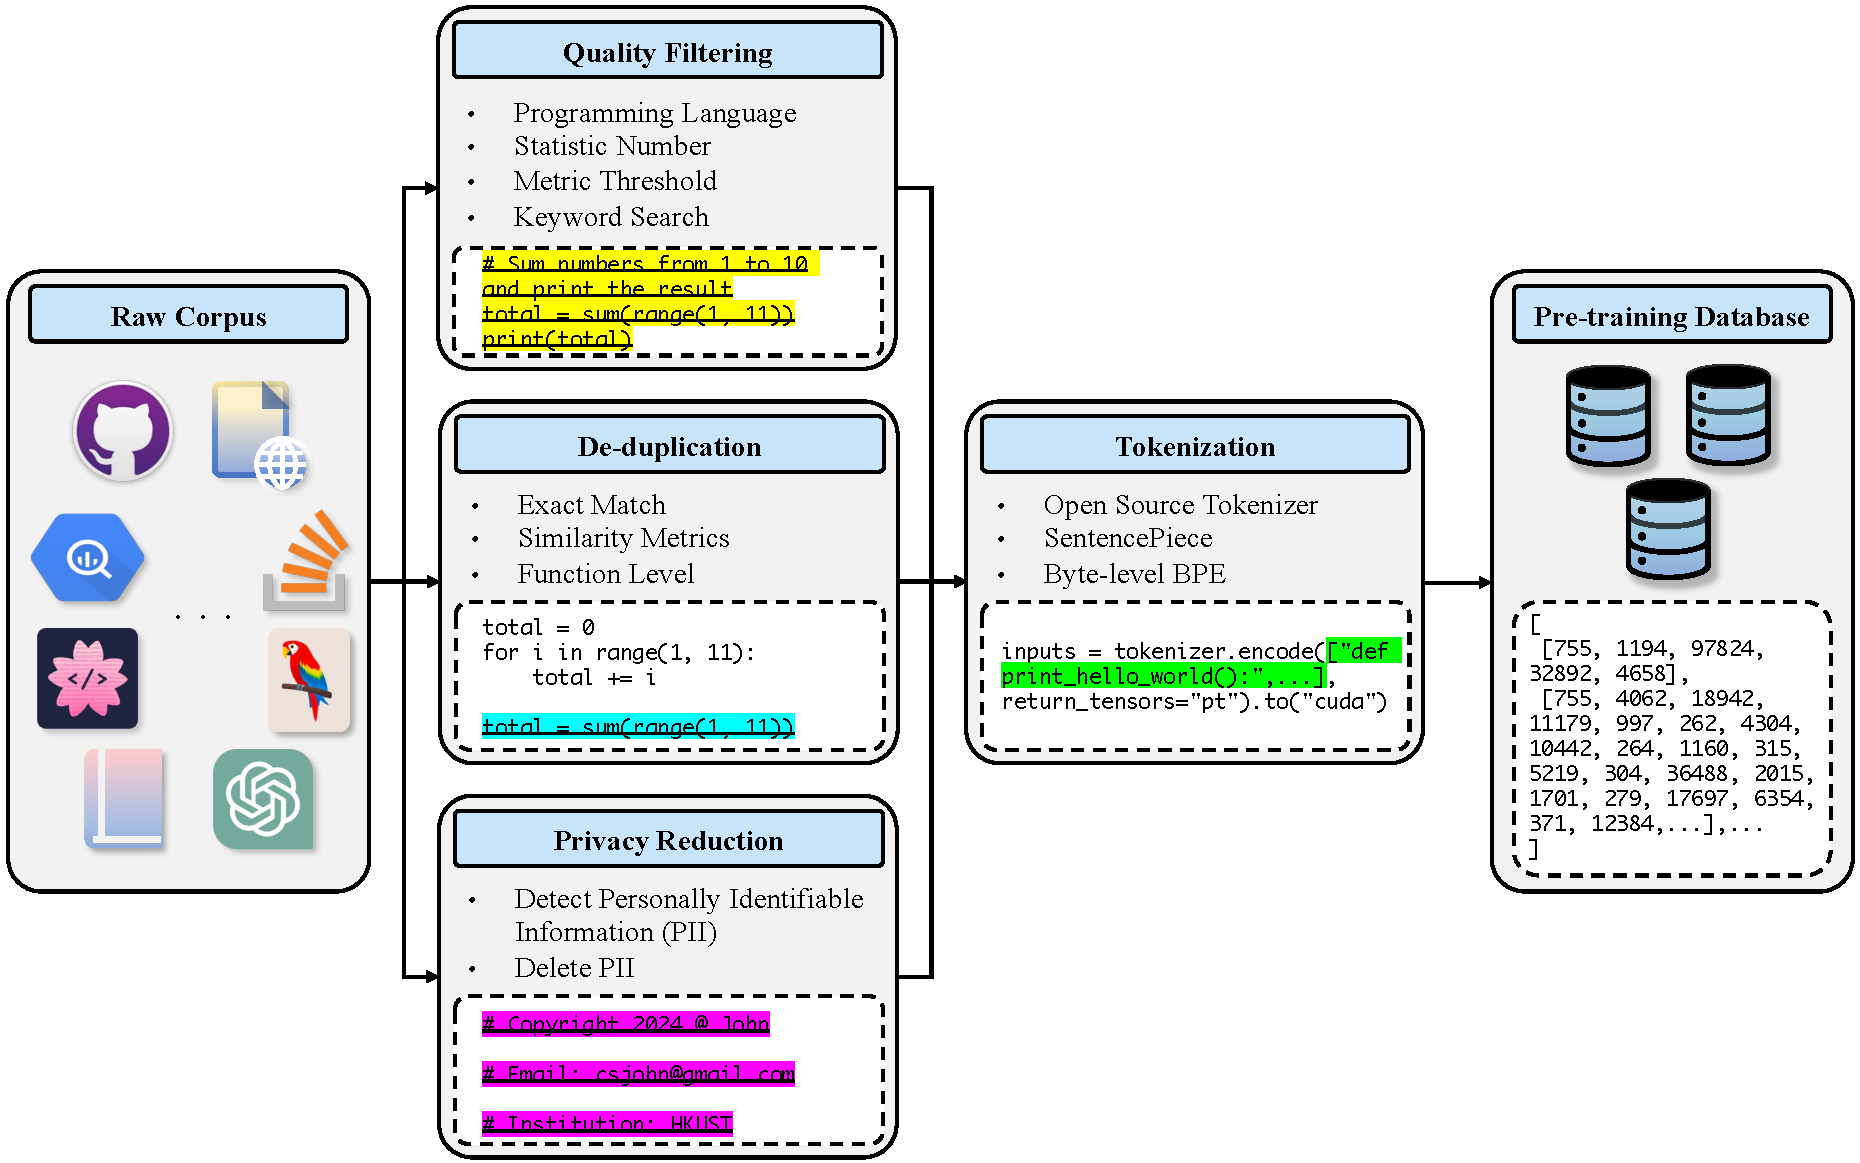
\includegraphics[width=\linewidth]{images/DataProcessing.pdf}
\caption{A diagram depicting the standard data preprocessing workflow utilized in the pre-training phase of \done{LLMs} for code generation.}
\label{fig:datapipeline}
\end{figure*}

\subsubsection{Pre-training}
% Due to the great success of bidirectional PLMs (e.g., BERT \cite{devlin2018bert}) and unidirectional PLMs (e.g., GPT \cite{radford2018improving}), pre-training on large-scale unlabelled dataset has been a prevalent training strategy to acquire general knowledge. 
% Employing this principle in the code domain helps LLM acquire basic coding concepts, such as code structure dependencies, code identifier meanings, and code internal logic \cite{chen2021evaluating,wang2021codet5,guo2022unixcoder,wang2023codet5+}.
% Therefore, an increasing number of large-scale unlabeled code datasets for LLMs have been proposed as follows while the statistics are summarized in Table \ref{tab:pretraining_dataset}:
The remarkable success of bidirectional pre-trained language models (PLMs) such as BERT \cite{devlin2018bert} and unidirectional PLMs like GPT \cite{radford2018improving} has firmly established the practice of pre-training on large-scale unlabeled datasets to endow models with a broad spectrum of general knowledge. 
Extending this principle to the realm of code generation enables \done{LLMs} to assimilate fundamental coding principles, including the understanding of code structure dependencies, the semantics of code identifiers, and the intrinsic logic of code sequences \cite{chen2021evaluating,wang2021codet5,guo2022unixcoder,wang2023codet5+}.
In light of this advancement, there has been a proliferation of large-scale unlabeled code datasets proposed to serve as the foundational training ground for LLMs to develop coding proficiency. 
% A comprehensive overview of these datasets, along with their key characteristics, 
A brief introduction of these datasets is as follows, with the statistics available in Table \ref{tab:pretraining_dataset}.

\begin{itemize}
    \item CodeSearchNet \cite{husain2019codesearchnet}: CodeSearchNet corpus is a comprehensive dataset, consisting of 2 million (comment, code) pairs from open-source repositories on GitHub. It includes code and documentation in several programming languages including Go, Java, PHP, Python, JavaScript, and Ruby. The dataset was primarily compiled to promote research into the problem of code retrieval using natural language.
    \item Google BigQuery \cite{hoffa2016github}: the Google BigQuery Public Datasets program offers a full snapshot of the content of more than 2.8 million open source GitHub repositories in BigQuery.
    \item The Pile \cite{gao2020pile}: the Pile is an 825 GiB diverse and open source language modeling dataset aggregating 22 smaller, high-quality datasets including GitHub, Books3, and Wikipedia (en). It aims to encompass text from as many modalities as possible, thereby facilitating the development of models with broader generalization capabilities. For code generation, the GitHub composite is specifically utilized.
    \item CodeParrot \cite{tunstall2022natural}: the CodeParrot dataset contains Python files used to train the code generation model in Chapter 10: Training Transformers from Scratch in the ``NLP with Transformers book'' \cite{tunstall2022natural}. Created with the GitHub dataset available via Google's BigQuery, the CodeParrot dataset includes approximately 22 million Python files and is 180 GB (50 GB compressed) big. 
    \item GitHub Code \cite{tunstall2022natural}: the GitHub Code dataset comprises 115M code files derived from GitHub, spanning 32 programming languages and 60 extensions totaling 1TB of data. The dataset was created from the public GitHub dataset on Google BiqQuery.
    \item ROOTS \cite{laurenccon2022bigscience}: the BigScience ROOTS Corpus is a 1.6TB dataset spanning 59 languages that was used to train the 176B BigScience Large Open-science Open-access Multilingual (BLOOM) language model. For the code generation task, the code subset of the ROOTS Corpus will be specifically utilized.  
    \item The Stack \cite{kocetkov2022stack}: the Stack contains over 6TB of permissively licensed source code files that cover 358 programming languages. The dataset was compiled as part of the BigCode Project, an open scientific collaboration working on the responsible development of Large Language Models for Code (Code LLMs).
    \item The Stack v2 \cite{lozhkov2024starcoder}: The Stack v2, a dataset created as part of the BigCode Project, contains over 3B files across more than 600 programming and markup languages. The dataset is derived from the Software Heritage archive\footnote{\href{https://archive.softwareheritage.org/}{https://archive.softwareheritage.org}}, the largest public archive of software source code and accompanying development history.
\end{itemize}

\begin{table}[t]
\caption{
% The statistics of some commonly-used pre-training datasets for pre-training large language models for code generation. The \textbf{\#PL} denotes the number of programming languages. Note that, each file is a function in CodeSearchNet \cite{husain2019codesearchnet} dataset, and we only consider their code composite for the Pile \cite{gao2020pile} and ROOTS \cite{laurenccon2022bigscience}.
The statistics of some commonly-used pre-training datasets for \done{LLMs} aimed at code generation. The column labeled `\textbf{\#PL}' indicates the number of programming languages included in each dataset. It should be noted that in the CodeSearchNet \cite{husain2019codesearchnet} dataset, each file represents a function, and for the Pile \cite{gao2020pile} and ROOTS \cite{laurenccon2022bigscience} datasets, only the code components are considered.
}
\label{tab:pretraining_dataset}
\centering
\scalebox{0.73}{
\rotatebox{0}{
    \begin{tabular}{llllcl}
    \toprule
        \textbf{Dataset} & \textbf{Size (GB)} & \textbf{Files (M)} & \textbf{\#PL} & \textbf{Date} & \textbf{Link}\\
    \midrule
        CodeSearchNet \cite{husain2019codesearchnet} & 20 & 6.5 & 6  & 2022-01 & \url{https://huggingface.co/datasets/code_search_net}\\
        Google BigQuery\cite{hoffa2016github}  & - & - & - & 2016-06 & \href{https://cloud.google.com/blog/topics/public-datasets/github-on-bigquery-analyze-all-the-open-source-code}{\url{github-on-bigquery-analyze-all-the-open-source-code}} \\
        The Pile \cite{gao2020pile} & 95 & 19 & - &  2022-01 & \url{https://huggingface.co/datasets/EleutherAI/pile}\\
        CodeParrot \cite{tunstall2022natural} & 180 & 22 & 1 & 2021-08 & \url{https://huggingface.co/datasets/transformersbook/codeparrot}\\
        GitHub Code\cite{tunstall2022natural} & 1,024 & 115 & 32 & 2022-02 & \url{https://huggingface.co/datasets/codeparrot/github-code}\\
        ROOTS \cite{laurenccon2022bigscience} & 163 & 15 & 13 & 2023-03 & \url{https://huggingface.co/bigscience-data} \\
        The Stack \cite{kocetkov2022stack} & 3,136 & 317 & 30 & 2022-10 & \url{https://huggingface.co/datasets/bigcode/the-stack}\\
        The Stack v2 \cite{lozhkov2024starcoder} & 32K & 3K & 619 & 2024-04 & \url{https://huggingface.co/datasets/bigcode/the-stack-v2}\\
    \bottomrule
    \end{tabular}
}
}
\end{table}

\subsubsection{Instruction Tuning}\label{sec:instruction_data}
% Instruction tuning refers to finetuning large language models on a collection of datasets phrased as instructions. It has been shown to improve model performance and generalization to unseen tasks significantly \cite{ouyang2022training,chung2024scaling}. 
% Because of this advantage, instruction tuning has been extended to code domains, particularly for code generation task, which aims to generate the intended code from natural language description automatically, and has attracted many researchers to construct large-scale code instruction-tuning datasets. In the following, we briefly introduce several representative datasets for instruction-tuning and provide the statistics in Table \ref{tab:instruction_dataset}.
\done{Instruction tuning refers to the process of supervised fine-tuning \done{LLMs} using a collection of datasets structured as various instructions, with the purpose of following a wide range of task instructions \cite{wei2021finetuned,sanh2022multitask,ouyang2022training,chung2024scaling}.
}
This method has demonstrated a considerable improvement in model performance and an enhanced ability to generalize to unseen tasks that the model has not previously encountered, as evidenced by recent studies \cite{ouyang2022training,chung2024scaling}.
Leveraging the benefits of instruction tuning, instruction tuning has been expanded into coding domains, especially for code generation, which involves the automatic generation of the intended code from a natural language description. The promise of instruction tuning in this area has led numerous researchers to develop large-scale instruction-tuning datasets tailored for code generation. 
Below, we provide an overview of several notable datasets tailored for instruction tuning, with their respective statistics detailed in Table \ref{tab:instruction_dataset}.

\begin{itemize}
    \item CodeAlpaca-20k \cite{codealpaca}: CodeAlpaca-20k is a collection of 20K instruction-following data generated using the data synthesis techniques termed Self-Instruct outlined in \cite{wang2023self}, with modifications for code generation, editing, and optimization tasks instead of general tasks. 
    \item CommitPackFT \cite{muennighoff2023octopack}: CommitPackFT is a 2GB refined version of CommitPack. It is filtered to only include high-quality commit messages that resemble natural language instructions.
    % \item oa\_leet10k \cite{oa-leet10k} % oa_leet10k: https://huggingface.co/datasets/ehartford/oa_leet10k 
    % \item EditPackFT
    \item Evol-Instruct-Code-80k \cite{evol_instruction}: Evol-Instruct-Code-80k is an open-source implementation of Evol-Instruct-Code described in the WizardCoder paper \cite{luo2023wizardcoder}, which enhances the fine-tuning effect of pre-trained code large models by adding complex code instructions.
    \item Magicoder-OSS-Instruct-75k \cite{wei2023magicoder}: is a 75k synthetic data generated through OSS-Instruct with \texttt{gpt-3.5-turbo-1106} and used to train both Magicoder and Magicoder-S series models.
    \item Self-OSS-Instruct-SC2-Exec-Filter-50k \cite{starcoder2instruct}: Self-OSS-Instruct-SC2-Exec-Filter-50k is generated by StarCoder2-15B using the OSS-Instruct \cite{wei2023magicoder} data synthesis approach. It was subsequently used to fine-tune StarCoder-15B without any human annotations or distilled data from huge and proprietary LLMs.
    % \item EditPackFT-Multi
\end{itemize}

% \subsubsection{Reinforcement Learning with Feedback}
\begin{table}[t]
\caption{
% Statistics of several pretraining datasets for code models: size in bytes, number of files, and number of programming languages. In CodeSearchNet each file is a function. For Pile and ROOTS we only consider their code composite.
The statistics of several representative datasets used in instruction-tuning \done{LLMs} for code generation. The column labeled `\textbf{\#PL}' indicates the number of programming languages encompassed by each dataset. 
}
\label{tab:instruction_dataset}
\centering
\scalebox{0.6}{
\rotatebox{0}{
    \begin{tabular}{lllll}
    \toprule
        \textbf{Dataset} & \textbf{Size} & \textbf{\#PL} & \textbf{Date} & \textbf{Link}\\
    \midrule
        CodeAlpaca-20K \cite{codealpaca} & 20k &  -  & 2023-03  & \url{https://huggingface.co/datasets/sahil2801/CodeAlpaca-20k}\\
        CommitPackFT \cite{muennighoff2023octopack} & 2GB & 277  & 2023-08  & \url{https://huggingface.co/datasets/bigcode/commitpackft}\\
        Evol-Instruct-Code-80k \cite{evol_instruction} & 80k &  - & 2023-07 & \url{https://huggingface.co/datasets/nickrosh/Evol-Instruct-Code-80k-v1}\\
        evol-codealpaca-v1 \cite{evol-codealpaca-v1} & 110K & - & 2023-07 & \href{https://huggingface.co/datasets/theblackcat102/evol-codealpaca-v1}{https://huggingface.co/datasets/theblackcat102/evol-codealpaca-v1}\\
        Magicoder-OSS-Instruct-75k \cite{wei2023magicoder} & 75k & \begin{tabular}[c]{@{}l@{}}Python, Shell, \\TypeScript, C++, \\Rust, PHP, Java, \\Swift, C\#\end{tabular}  & 2023-12 & \url{https://huggingface.co/datasets/ise-uiuc/Magicoder-OSS-Instruct-75K}\\
        \makecell[l]{Self-OSS-Instruct-SC2-Exec-Filter-50k \cite{starcoder2instruct}} & 50k &  Python  & 2024-04  & \url{https://huggingface.co/datasets/bigcode/self-oss-instruct-sc2-exec-filter-50k}\\
    \bottomrule
    \end{tabular}
}
}
\end{table}

\subsubsection{Benchmarks}\label{sec:benchmark}
% To evaluate the performance of LLM on code generation tasks, a series of high-quality benchmarks have been proposed in recent years. Pioneered by \cite{chen2021evaluating}, a lot of variants of HumanEval and new benchmarks have been proposed to evaluate more aspects of code on LLM. We roughly divide these benchmarks into six categories according to their application scenarios, including general-purpose, competitions, data science, multilingual, reasoning, and repository-level. The detailed statistics of these benchmarks are displayed in Table. \ref{tab:benchmark}.
To rigorously assess the efficacy of \done{LLMs} for code generation, the research community has introduced a variety of high-quality benchmarks in recent years. 
Building on the foundational work by \cite{chen2021evaluating}, numerous variations of the HumanEval dataset and additional benchmarks have emerged, aiming to evaluate a broader spectrum of code generation capabilities in LLMs. 
We roughly divide these benchmarks into six distinct categories based on their application contexts, including general-purpose, competitive programming, data science, multilingual, logical reasoning, and repository-level. 
\done{
% It is important to note that for logical reasoning, it involves math-related benchmarks 
% since it aims to generate code-based solutions for solving challenging math problems \cite{chen2022program,gao2023pal,zhou2023solving}.
% Thus, it can compensate for LLMs' limitations in doing complex math computations.
% It is important to emphasize that logical reasoning includes math-related benchmarks, as it seeks to develop code-based solutions for tackling complex mathematical problems \cite{chen2022program,gao2023pal,zhou2023solving}. 
% Consequently, this approach can address the limitations of LLMs in performing intricate mathematical computations.
It is important to highlight that logical reasoning encompasses math-related benchmarks, as it aims to create ``code-based solutions'' for solving complex mathematical problems \cite{chen2022program,gao2023pal,zhou2023solving}. This strategy can therefore mitigate the limitations of LLMs in performing intricate mathematical computations.
}
The statistics for these benchmarks are presented in Table \ref{tab:benchmark}.

\textbf{General}
\begin{itemize}
    \item HumanEval \cite{chen2021evaluating}: HumanEval comprises 164 manually scripted Python programming problems, each featuring a function signature, docstring, body, and multiple unit tests.
    \item HumanEval+ \cite{liu2024your}: HumanEval+ extends the original HumanEval \cite{chen2021evaluating} benchmark by increasing the scale of the test cases by 80 times. As the test cases increase, HumanEval+ can catch significant amounts of previously undetected incorrect code synthesized by LLMs.
    \item HumanEvalPack \cite{muennighoff2023octopack}: expands HumanEval \cite{chen2021evaluating} by extending it to encompass three coding tasks across six programming languages, namely code synthesis, code repair, and code explanation. 
    \item MBPP \cite{austin2021program}: MBPP is a collection of approximately 974 Python programming problems, crowd-sourced and designed for entry-level programmers. Each problem comes with an English task description, a code solution, and three automated test cases. 
    \item MBPP+ \cite{liu2024your}: MBPP+ enhances MBPP \cite{austin2021program} by eliminating ill-formed problems and rectifying problems with incorrect implementations. The test scale of MBPP+ is also expanded by 35 times for test augmentation.
    \item CoNaLa \cite{yin2018learning}: CoNaLa contains almost 597K data samples for evaluating Python code generation. The curated part of CoNaLa is crawled from Stack Overflow, automatically filtered, and then curated by annotators. The mined part of CoNaLais automatically mined, with almost 600k examples.
    \item Spider \cite{yu2018spider}: Spider is large-scale complex text-to-SQL dataset covering 138 different domains. It has over 10K questions and 5.6K complex SQL queries on 200 databases. This dataset aims to test a model's ability to generalize to SQL queries, database schemas, and new domains.
    \item CONCODE \cite{iyer2018mapping}: CONCODE is a dataset with over 100K samples consisting of Java classes from public GitHub repositories. It provides near zero-shot conditions that can test the model's ability to generalize to unseen natural language tokens with unseen environments.
    \item ODEX \cite{wang2022execution}: ODEX is an open-domain dataset focused on the execution-based generation of Python code from natural language. It features 945 pairs of natural language queries and their corresponding Python code, all extracted from StackOverflow forums.
    \item CoderEval \cite{yu2024codereval}: CoderEval is a pragmatic code generation benchmark that includes 230 Python and 230 Java code generation problems. It can be used to evaluate the model performance in generating pragmatic code beyond just generating standalone functions.
    \item ReCode \cite{wang2022recode}: Recode serves as a comprehensive robustness evaluation benchmark. ReCode applies perturbations to docstrings, function and variable names, code syntax, and code format, thereby providing multifaceted assessments of a model's robustness performance. 
    % proposes a set of code and natural language transformations to evaluate the robustness of code-generation models. 
    % The perturbations can be applied to any code-generation benchmark. Specifically, they release perturbed versions of HumanEval \cite{chen2021evaluating} and MBPP \cite{austin2021program}.
    \item StudentEval \cite{babe2023studenteval}: StudentEval is a dataset of 1,749 prompts for 48 problems, authored by 80 students who have only completed a one-semester Python programming class. Unlike many other benchmarks, it has multiple prompts per problem and multiple attempts by the same participant, each problem is also accompanied by a set of instructor-written test cases.
    \done{\item BigCodeBench \cite{zhuo2024bigcodebench}: BigCodeBench has 1,140 complex Python programming tasks, covering 723 function calls from 139 popular libraries across 7 domains. This benchmark is specifically designed to assess LLMs' ability to call multiple functions from cross-domain libraries and follow complex instructions to solve programming tasks, helping to bridge the evaluation gap between isolated coding exercises and the real-world programming scenario.}
    \done{\item ClassEval \cite{du2024evaluating}: ClassEval is a manually-crafted benchmark consisting of 100 classes and 412 methods for evaluating LLMs in the class-level code generation scenario. Particularly, the task samples of ClassEval present higher complexities, involving long code generation and sophisticated docstring information, thereby benefiting the evaluation of the LLMs' capabilities in generating complicated code.}
    \done{\item NaturalCodeBench \cite{zhang2024naturalcodebench}: NaturalCodeBench is a comprehensive code benchmark featuring 402 high-quality problems in Python and Java. These problems are selected from natural user queries from online coding services and span 6 distinct domains, shaping an evaluation environment aligned with real-world applications.}
\end{itemize}

\textbf{Competitions}
\begin{itemize}
    \item APPS \cite{hendrycks2021measuring}: The APPS benchmark is composed of 10K Python problems, spanning three levels of difficulty: introductory, interview, and competition. Each entry in the dataset includes a programming problem described in English, corresponding ground truth Python solutions, test cases defined by their inputs and outputs or function names if provided.
    \item CodeContests \cite{li2022competition}: CodeContests is a competitive programming dataset consisting of samples from various sources including Aizu, AtCoder, CodeChef, Codeforces, and HackerEarth. The dataset encompasses programming problems accompanied by test cases in the form of paired inputs and outputs, along with both correct and incorrect human solutions in multiple programming languages.
    \done{\item LiveCodeBench \cite{naman2024livecodebench}: LiveCodeBench is a comprehensive and contamination-free benchmark for evaluating a wide array of code-related capabilities of LLMs, including code generation, self-repair, code execution, and test output prediction. It continuously gathers new coding problems from contests across three reputable competition platforms: LeetCode, AtCoder, and CodeForces. The latest release of the dataset includes 713 problems that were released between May 2023 and September 2024.
    }
\end{itemize}

\textbf{Data Science}
\begin{itemize}
    \item DSP \cite{chandel2022training}: DSP allows for model evaluation based on real data science pedagogical notebooks. It includes well-structured problems, along with unit tests to verify the correctness of solutions and a Docker environment for reproducible execution.
    \item DS-1000 \cite{lai2023ds}: DS-1000 has 1K science questions from seven Python libraries, namely NumPy, Pandas, TensorFlow, PyTorch, SciPy, Scikit-learn, and Matplotlib. The DS-1000 benchmark features: (1) realistic problems with diverse contexts (2) implementation of multi-criteria evaluation metrics, and (3) defense against memorization.
    \item ExeDS \cite{huang2022execution}: ExeDS is a data science code generation dataset specifically designed for execution evaluation. It contains 534 problems with execution outputs from Jupyter Notebooks, as well as 123K examples for training and validation.
\end{itemize}

\textbf{Multilingual}
\begin{itemize}
    \item MBXP \cite{athiwaratkun2022multi}: MBXP is a multilingual adaptation of the original MBPP \cite{austin2021program} dataset. It is created using a framework that translates prompts and test cases from the original Python datasets into the corresponding data in the targeted programming language.
    \item Multilingual HumanEval \cite{athiwaratkun2022multi}: Multilingual HumanEval is a dataset derived from HumanEval \cite{chen2021evaluating}. It is designed to assess the performance of models in a multilingual context.
    It helps uncover the generalization ability of the given model on languages that are out-of-domain.
    \item HumanEval-X \cite{zheng2023codegeex}: HumanEval-X is developed for evaluating the multilingual ability of code generation models with 820 hand-writing data samples in C++, Java, JavaScript, and Go.
    \item MultiPL-E \cite{cassano2022scalable}: 
    % extends HumanEval \cite{chen2021evaluating} and MBPP \cite{austin2021program} to 18 languages that encompass a range of programming paradigms and popularity.
    MultiPL-E is a dataset for evaluating LLMs for code generation across 18 programming languages. It adopts the HumanEval \cite{chen2021evaluating} and the MBPP \cite{austin2021program} Python benchmarks and uses little compilers to translate them to other languages.
    \item xCodeEval \cite{khan2023xcodeeval}: xCodeEval is an executable multilingual multitask benchmark consisting of 25M examples covering 17 programming languages. Its tasks include code understanding, generation, translation, and retrieval.
\end{itemize}

\textbf{Reasoning}
\begin{itemize}
    \item MathQA-X \cite{athiwaratkun2022multi} MathQA-X is the multilingual version of MathQA \cite{amini2019mathqa}. It is generated by utilizing a conversion framework that converts samples from Python datasets into the target language.
    \item MathQA-Python \cite{austin2021program} MathQA-Python is a Python version of the MathQA benchmark\cite{amini2019mathqa}. The benchmark, containing more than 23K problems, is designed to assess the capability of models to synthesize code from complex textual descriptions.
    \item GSM8K \cite{cobbe2021training}: GSM8K is a dataset of 8.5K linguistically diverse grade school math problems. The dataset is crafted to facilitate the task of question answering on basic mathematical problems that requires multi-step reasoning.
    \item GSM-HARD \cite{gao2023pal}: GSM-HARD is a more challenging version of the GSM8K \cite{cobbe2021training} dataset. It replaces the numbers in the GSM8K questions with larger, less common numbers, thereby increasing the complexity and difficulty level of the problems.
    \done{\item CRUXEval \cite{gu2024cruxeval}: CRUXEval contains 800 Python functions, each paired with an input-output example. This benchmark supports two tasks: input prediction and output prediction, designed to evaluate the code reasoning, understanding, and execution capabilities of code LLMs.}
\end{itemize}

\begin{table}[t]
\caption{
The detailed statistics of commonly-used benchmarks used in evaluating \done{LLMs} for code generation. 
The column labeled `\textbf{\#PL}' indicates the number of programming languages included in each dataset. For the sake of brevity, we list the programming languages (PLs) for benchmarks that support fewer than or include five PLs. For benchmarks with six or more PLs, we provide only a numerical count of the PLs supported.
}
\label{tab:benchmark}
\centering
\scalebox{0.63}{
\rotatebox{0}{
    \begin{tabular}{llllcl}
    \toprule
        \textbf{Scenario} & \textbf{Benchmark} & \textbf{Size} & \textbf{\#PL} & \textbf{Date} & \textbf{Link}\\
    \midrule
        \multirow{15}*{General}& HumanEval \cite{chen2021evaluating} &164&Python& 2021-07&\url{https://huggingface.co/datasets/openai_humaneval}\\
         & HumanEval+ \cite{liu2024your} &164&Python&2023-05&\url{https://huggingface.co/datasets/evalplus/humanevalplus}\\
         & HumanEvalPack \cite{muennighoff2023octopack} &164&6&2023-08&\url{https://huggingface.co/datasets/bigcode/humanevalpack}\\
         & MBPP \cite{austin2021program} &974&Python&2021-08&\url{https://huggingface.co/datasets/mbpp}\\
         & MBPP+ \cite{liu2024your} &378&Python&2023-05&\url{https://huggingface.co/datasets/evalplus/mbppplus}\\
         & CoNaLa \cite{yin2018learning} &596.88K&Python&2018-05&\url{https://huggingface.co/datasets/neulab/conala}\\
         & Spider \cite{yu2018spider} &8,034&SQL&2018-09&\url{https://huggingface.co/datasets/xlangai/spider}\\
         & CONCODE \cite{iyer2018mapping} &104K&Java&2018-08&\href{https://huggingface.co/datasets/AhmedSSoliman/CodeXGLUE-CONCODE}{\url{https://huggingface.co/datasets/AhmedSSoliman/CONCOD}}\\
         & ODEX \cite{wang2022execution} &945&Python&2022-12&\url{https://huggingface.co/datasets/neulab/odex}\\
         & CoderEval \cite{yu2024codereval} &460&Python, Java&2023-02&\url{https://github.com/CoderEval/CoderEval}\\
         & ReCode \cite{wang2022recode} &1,138&Python&2022-12&\url{https://github.com/amazon-science/recode}\\
         & StudentEval \cite{babe2023studenteval} &1,749&Python&2023-06&\url{https://huggingface.co/datasets/wellesley-easel/StudentEval} \\
         & \done{BigCodeBench \cite{zhuo2024bigcodebench}} & \done{1,140} & \done{Python} & \done{2024-06}& \done{\url{https://huggingface.co/datasets/bigcode/bigcodebench}} \\
         & \done{ClassEval \cite{du2024evaluating}} &\done{100} & \done{Python} & \done{2023-08}&\done{\url{https://huggingface.co/datasets/FudanSELab/ClassEval}} \\
         & \done{NaturalCodeBench \cite{zhang2024naturalcodebench}} &\done{402} & \done{Python, Java} & \done{2024-05}&\done{\url{https://github.com/THUDM/NaturalCodeBench}} \\
    \midrule
        \multirow{3}*{Competitions} & APPS \cite{hendrycks2021measuring} &10,000&Python&2021-05&\url{https://huggingface.co/datasets/codeparrot/apps} \\
        & CodeContests \cite{li2022competition} &13,610&\makecell[l]{C++, Python,\\ Java}&2022-02&\url{https://huggingface.co/datasets/deepmind/code_contests} \\
        & \done{LiveCodeBench \cite{naman2024livecodebench}} &\done{\makecell[l]{713\\ Updating}} & \done{Python} & \done{2024-03}&\done{\url{https://github.com/LiveCodeBench/LiveCodeBench}} \\
    \midrule
        \multirow{3}*{Data Science} & DSP \cite{chandel2022training} &1,119&Python&2022-01&\url{https://github.com/microsoft/DataScienceProblems}\\
        & DS-1000 \cite{lai2023ds} &1,000&Python&2022-11&\url{https://huggingface.co/datasets/xlangai/DS-1000} \\
        & ExeDS \cite{huang2022execution} &534&Python&2022-11&\url{https://github.com/Jun-jie-Huang/ExeDS} \\
    \midrule
        \multirow{5}*{Multilingual} & MBXP \cite{athiwaratkun2022multi}  &12.4K&13&2022-10&\url{https://huggingface.co/datasets/mxeval/mbxp} \\
        & Multilingual HumanEval \cite{athiwaratkun2022multi}  &1.9K&12&2022-10&\url{https://huggingface.co/datasets/mxeval/multi-humaneval} \\
        & HumanEval-X \cite{zheng2023codegeex}  &820&\makecell[l]{Python, C++, \\Java, JavaScript,\\ Go}&2023-03&\url{https://huggingface.co/datasets/THUDM/humaneval-x} \\
        & MultiPL-E \cite{cassano2022scalable}  &161&18&2022-08&\url{https://huggingface.co/datasets/nuprl/MultiPL-E} \\
        & xCodeEval \cite{khan2023xcodeeval}  &5.5M&11&2023-03&\url{https://github.com/ntunlp/xCodeEval} \\
    \midrule
        \multirow{5}*{Reasoning} & MathQA-X \cite{athiwaratkun2022multi}  &5.6K& \makecell[l]{Python, Java, \\JavaScript} &2022-10&\url{https://huggingface.co/datasets/mxeval/mathqa-x} \\
        & MathQA-Python \cite{austin2021program} &23,914&Python&2021-08& \url{https://github.com/google-research/google-research} \\
        & GSM8K \cite{cobbe2021training} &8.5K&Python&2021-10&\url{https://huggingface.co/datasets/gsm8k} \\
        & GSM-HARD \cite{gao2023pal} &1.32K&Python&2022-11&\url{https://huggingface.co/datasets/reasoning-machines/gsm-hard} \\
        & \done{CRUXEval \cite{gu2024cruxeval}} &\done{800} & \done{Python} & \done{2024-01}&\done{\url{https://huggingface.co/datasets/cruxeval-org/cruxeval}} \\
    \midrule
        \multirow{7}*{Repository} & RepoEval \cite{zhang2023repocoder} &3,573&Python, Java&2023-03&\url{https://paperswithcode.com/dataset/repoeval} \\
        & Stack-Repo \cite{shrivastava2023repofusion} & 200 &Java&2023-06&\url{https://huggingface.co/datasets/RepoFusion/Stack-Repo} \\
        & Repobench \cite{liu2023repobench} & 27k  &Python, Java&2023-01&\url{https://github.com/Leolty/repobench} \\
        & EvoCodeBench \cite{li2024evocodebench} &275&Python&2024-03&\url{https://huggingface.co/datasets/LJ0815/EvoCodeBench}\\
        & SWE-bench \cite{jimenez2023swe} &2,294&Python&2023-10&\url{https://huggingface.co/datasets/princeton-nlp/SWE-bench} \\
        & CrossCodeEval \cite{ding2024crosscodeeval} &10K&\makecell[l]{Python, Java,\\ TypeScript, C\#}&2023-10&\url{https://github.com/amazon-science/cceval} \\
        & SketchEval \cite{zan2024codes} &20,355&Python&2024-03&\url{https://github.com/nl2code/codes} \\
    \bottomrule
    \end{tabular}
}
}
\end{table}
\textbf{Repository}
\begin{itemize}
    \item RepoEval \cite{zhang2023repocoder}: RepoEval enables the evaluation of repository-level code completion. It can offer different levels of granularity and improved evaluation accuracy through the use of unit tests.
    \item Stack-Repo \cite{shrivastava2023repofusion}: Stack-Repo is a dataset of 200 Java repositories from GitHub with near-deduplicated files. These files are augmented with three types of repository contexts: prompt proposal contexts, BM25 Contexts (based on BM25 similarity scores), and RandomNN Contexts (obtained using the nearest neighbors in the representation space of an embedding model).
    \item Repobench \cite{liu2023repobench}: Repobench is a benchmark specifically used for evaluating repository-level code auto-completion systems. Supporting both Python and Java, it consists of three interconnected evaluation tasks: RepoBench-R (Retrieval), RepoBench-C (Code Completion), and RepoBench-P (Pipeline).
    \item EvoCodeBench \cite{li2024evocodebench}: EvoCodeBench is an evolutionary code generation benchmark, constructed through a rigorous pipeline and aligned with real-world repositories. This benchmark also provides comprehensive annotations and robust evaluation metrics.
    \item SWE-bench \cite{jimenez2023swe}: SWE-bench is a dataset that tests a model’s ability to automatically solve GitHub issues. The dataset has 2,294 Issue-Pull Request pairs from 12 popular Python repositories.
    \item CrossCodeEval \cite{ding2024crosscodeeval}: CrossCodeEval is a diverse and multilingual scope completion dataset covering four languages: Python, Java, TypeScript, and C\#. This benchmark tests the model's ability to understand in-depth cross-file information and accurately complete the code. 
    \item SketchEval \cite{zan2024codes}: SketchEval is a repository-oriented benchmark that encompasses data from 19 repositories, each varying in complexity. In addition to the dataset, SketchEval introduces a metric, known as SketchBLEU, to measure the similarity between two repositories based on their structures and semantics. 
\end{itemize}

%%%%%%%%%%%%%%%%%%%%%%%%%%%%%%%%%%%%%%%%%%%%%%%%%%%%%%%%%%%%%%%%%%%%%%%%
%%%%%%%%%%%%%%%%%%%%%%%%%%%%%%%%%%%%%%%%%%%%%%%%%%%%%%%%%%%%%%%%%%%%%%%%
\subsection{Data Synthesis}\label{sec:data_synthesis}
\begin{figure*}[t]
\centering
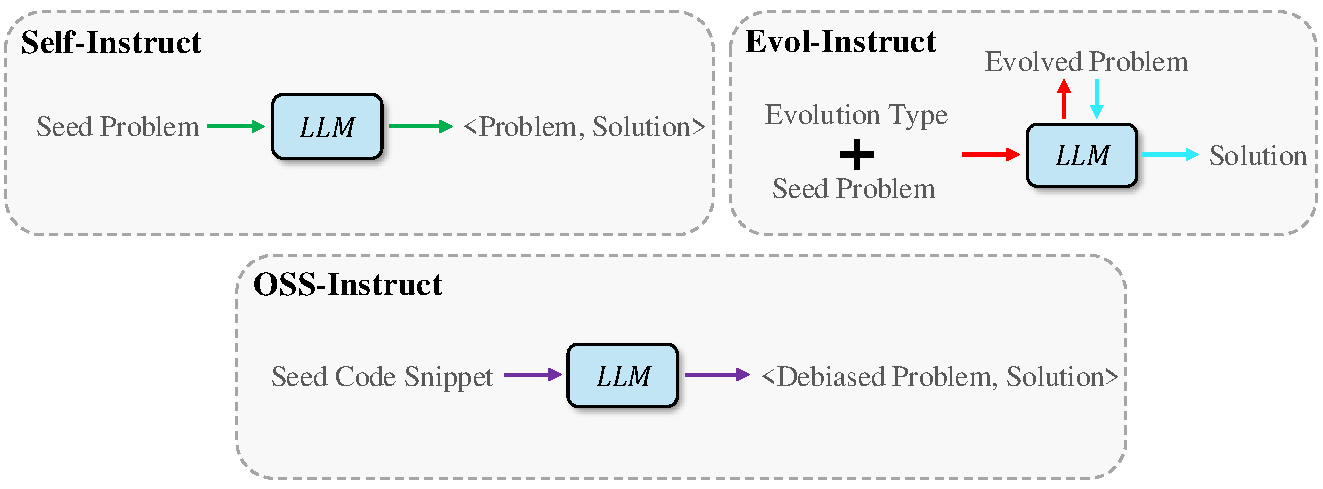
\includegraphics[width=\linewidth]{images/data_synthesis_v2.pdf}
\caption{\done{The comparison among three representative data synthesis methods used for generating instruction data with LLMs. The Code Alpaca \cite{codealpaca} employs the self-instruct method, whereas WizardCoder \cite{luo2023wizardcoder} and Magicoder \cite{wei2023magicoder} utilize the Evol-Instruct and OSS-Instruct methods, respectively.}}
\label{fig:data_synthesis}
\end{figure*}
% There have been many works proving that high-quality datasets drastically improve the performance of large language models in end tasks \cite{brown2020language,meng2022generating,xie2023data,zhou2024lima,kopf2024openassistant,wettig2024qurating}. 
% For example, LIMA \cite{zhou2024lima}, a 65B parameter LLaMa language model fine-tuned with the standard supervised loss on only 1,000 carefully curated prompts and responses, without any reinforcement learning or human preference modeling, achieves either equivalent or strictly preferred to GPT-4 in 43\% of cases, which is as high as 58\% when compared to Bard and 65\% versus DaVinci003. 
% QuRating \cite{wettig2024qurating} selects high-quality pre-training data based on four abstract qualities of texts - writing style, required expertise, facts \& trivia, and educational value which humans intuitively perceive, and then train a 1.3B-parameter language model on the selected data, achieving lower perplexity and stronger in-context learning performance than baselines. 
Numerous studies have demonstrated that high-quality datasets are integral to enhancing the performance of \done{LLMs} in various downstream tasks \cite{brown2020language,meng2022generating,xie2023data,zhou2024lima,kopf2024openassistant,wettig2024qurating}. 
For instance, the LIMA model, a 65B parameter LLaMa language model fine-tuned with a standard supervised loss on a mere 1,000 meticulously curated prompts and responses, achieved performance on par with, or even superior to, GPT-4 in 43\% of evaluated cases. This figure rose to 58\% when compared to Bard and 65\% against \texttt{DaVinci003}, all without the use of reinforcement learning or human preference modeling \cite{zhou2024lima}. 
The QuRating initiative strategically selects pre-training data embodying four key textual qualities — writing style, facts \& trivia, required expertise, and educational value — that resonate with human intuition. Training a 1.3B parameter model on such data resulted in reduced perplexity and stronger in-context learning compared to baseline models \cite{wettig2024qurating}.

% Despite this great success, quality data is challenging to obtain due to data scarcity, privacy concerns, and high costs \cite{wang2023self,liu2024best}. It’s laborious and expensive for humans to make, and typically lacks the depth and breadth that ChatBots need to guide them through difficult, rare, or ambiguous situations.
% To this end, synthetic data has emerged as a promising solution by generating artificial data, primarily using GPT-3.5-turbo \cite{gpt-3.5-turbo} and GPT-4 \cite{achiam2023gpt}, that mimics the characteristics and patterns of real-world data, leading to a human-annotation-free method \cite{wang2023self,hamalainen2023evaluating,liu2024best,moritzlaurer}.
% To improve the instruction-following capability of LLM, the type of synthetic data primarily encompasses instruction-following data.
Despite these advancements, acquiring quality data remains a significant challenge due to issues such as data scarcity, privacy concerns, and prohibitive costs \cite{wang2023self,liu2024best}. 
Human-generated data is often labor-intensive and expensive to produce, and it may lack the necessary scope and detail to navigate complex, rare, or ambiguous scenarios.
As a resolution to these challenges, synthetic data has emerged as a viable alternative. By generating artificial datasets that replicate the intricacies of real-world information, models such as \texttt{GPT-3.5-turbo} \cite{gpt-3.5-turbo} and \texttt{GPT-4} \cite{achiam2023gpt} have enabled the creation of rich datasets without the need for human annotation \cite{wang2023self,hamalainen2023evaluating,liu2024best,moritzlaurer}. This approach is particularly beneficial in enhancing the instruction-following capabilities of LLMs, with a focus on generating synthetic instruction-based data.

% For example, a pioneered work Self-Instruct \cite{wang2023self} first proposes a framework to generate instructions, input, and output samples from an off-the-shelf language model, then filters invalid or similar ones before using them to finetune the original model. 
% The empirical results show the effectiveness of data synthesis. 
% Followed by Self-Instruct, the Alpaca model is fine-tuned from a 7B LLaMA model \cite{touvron2023llama} on 52K instruction-following data and behaves similarly to the \texttt{text-davinci-003} model. Subsequently, WizardLM \cite{xu2023wizardlm} proposes a novel data synthesis technique of Evol-Instruct to rewrite the initial set of instructions step by step into more complex instructions. The fine-tuned LLaMA demonstrates a preferred response compared to proprietary LLM, e.g., ChatGPT and GPT4, to some extent. 
% Moreover, Microsoft pushes this field with their series of smaller-scale Phi models including Phi-1 (1.3B) \cite{gunasekar2023textbooks} for Python coding, Phi-1.5 (1.3B) \cite{li2023textbooks} for common sense reasoning and language understanding, Phi-2 (2.7B) \cite{phi-2} for reasoning and language understanding, and Phi-3 (3.8B) \cite{abdin2024phi} for general purpose, which was predominantly trained on synthetic data and consistently surpasses much larger models on a variety of benchmarks.
A notable example of this approach is the Self-Instruct \cite{wang2023self} framework, which employs an off-the-shelf language model to generate a suite of instructions, inputs, and outputs. 
This data is then refined by removing invalid or redundant entries before being used to fine-tune the model. The empirical evidence supports the efficacy of this synthetic data generation methodology. 
Building upon this concept, the Alpaca \cite{alpaca} model, fine-tuned on 52k pieces of instruction-following data from a 7B parameter LLaMa \cite{touvron2023llama} model, exhibits performance comparable to the \texttt{text-davinci-003} model. 
WizardLM \cite{xu2023wizardlm} introduced the Evol-Instruct technique, which incrementally transforms simple instructions into more complex variants. The fine-tuned LLaMa model using this technique has shown promising results in comparison to established proprietary LLMs such as ChatGPT \cite{gpt-3.5-turbo} and GPT-4 \cite{achiam2023gpt}, to some extent.
Moreover, Microsoft has contributed to this field with their Phi series of models, predominantly trained on synthetic high-quality data, which includes Phi-1 (1.3B) \cite{gunasekar2023textbooks} for Python coding, Phi-1.5 (1.3B) \cite{li2023textbooks} for common sense reasoning and language understanding, Phi-2 (2.7B) \cite{phi-2} for advanced reasoning and language understanding, and Phi-3 (3.8B) \cite{abdin2024phi} for general purposes. These models have consistently outperformed larger counterparts across various benchmarks, demonstrating the efficacy of synthetic data in model training.

% Inspired by synthesizing data for general-purpose LLM, some researchers have extended synthetic data for code generation tasks.  
% Code Alpaca model \cite{codealpaca} is fine-tuned from a 7B and 13B LLaMA model on 20K instruction-following data for code generation generated by text-davinci-003\footnote{\href{https://platform.openai.com/docs/deprecations}{https://platform.openai.com}} with Self-Instruct technique \cite{wang2023self}.
Drawing on the successes of data synthesis for general-purpose \done{LLMs}, researchers have expanded the application of synthetic data to the realm of code generation. The Code Alpaca model, as described in \cite{codealpaca}, has been fine-tuned on a 7B and 13B LLaMA model using a dataset of 20k instruction-following examples for code generation. This dataset was created by \texttt{text-davinci-003}\footnote{\href{https://platform.openai.com/docs/deprecations}{https://platform.openai.com}} and employed the Self-Instruct technique \cite{wang2023self}.
% WizardCoder 15B \cite{luo2023wizardcoder} adapts the Evol-Instruct technique to synthesize 78k evolved code instruction data\footnote{The seed data is initialized by 20k instruction-following dataset of Code Alpaca \cite{codealpaca} generated by \texttt{text-davinci-003}.} and then fine-tunes on StarCoder base model to achieve 57.3\% pass@1 on the HumanEval benchmarks, surpassing all other open-source Code LLMs by a substantial margin and the largest closed LLMs, Anthropic’s Claude and Google’s Bard.
Building on this, the WizardCoder 15B \cite{luo2023wizardcoder} utilizes the Evol-Instruct technique to create an enhanced dataset of 78k evolved code instruction examples. This dataset originates from the initial 20k instruction-following dataset used by Code Alpaca \cite{codealpaca}, which was also generated by \texttt{text-davinci-003}. 
The WizardCoder model, fine-tuned on the StarCoder \cite{li2023starcoder} base model, achieved a 57.3\% \texttt{pass@1} on the HumanEval benchmarks. 
This performance not only surpasses all other open-source Code LLMs by a significant margin but also outperforms leading closed LLMs such as Anthropic’s Claude and Google’s Bard.
% Further, Magicoder \cite{wei2023magicoder} proposes a novel data synthesis method OSS-INSTRUCT, which enlightens LLMs with open-source code snippets to generate high-quality instruction data for code, aiming to mitigate the inherent bias of the synthetic data generated by LLMs. Building upon CodeLlama \cite{roziere2023code}, MagicoderS-CL-7B fine-tuned on 75K synthetic instruction data using OSS-INSTRUCT technique with \texttt{gpt-3.5-turbo-1106} as generator surpasses the prominent ChatGPT on HumanEval Plus (66.5 vs. 65.9 in pass@1). 
In a similar vein, Magicoder \cite{wei2023magicoder} introduces a novel data synthesis approach termed OSS-INSTRUCT which enlightens LLMs with open-source code snippets to generate high-quality instruction data for coding tasks. It aims to address the inherent biases often present in synthetic data produced by LLMs. 
Building upon CodeLlama \cite{roziere2023code}, the MagicoderS-CL-7B model — fine-tuned with 75k synthetic instruction data using the OSS-INSTRUCT technique and with \texttt{gpt-3.5-turbo-1106} as the data generator — has outperformed the prominent ChatGPT on the HumanEval Plus benchmark, achieving \texttt{pass@1} of 66.5\% versus 65.9\%.
% Impressively, Microsoft proposes phi-1 \cite{gunasekar2023textbooks} with a significantly smaller size of 1.3B trained on a selection of textbook quality data from the web (6B tokens) and synthetically generated textbooks and exercises with GPT-3.5 (1B tokens) achieves pass@1 accuracy 50.6\% on HumanEval and 55.5\% on MBPP, setting a new state-of-the-art performance on Python coding among existing small language models (SLMs).
In a noteworthy development, Microsoft has introduced the phi-1 model \cite{gunasekar2023textbooks}, a more compact LLM of only 1.3B parameters. Despite its smaller size, phi-1 has been trained on high-quality textbook data sourced from the web (comprising 6 billion tokens) and supplemented with synthetic textbooks and exercises generated with GPT-3.5 (1 billion tokens). It has achieved \texttt{pass@1} of 50.6\% on HumanEval and 55.5\% on MBPP, setting a new state-of-the-art for Python coding performance among existing small language models (SLMs).
% Most recently, the BigCode team presented the StarCoder2-15B-instruct \cite{starcoder2instruct}, the very first entirely self-aligned code \done{LLM} trained with a fully permissive and transparent pipeline. 
% To be specific, StarCoder2-15B-instruct essentially follows the principle of OSS-INSTRUCT proposed by Magicoder to generate instruction based on seed functions filtered from Stack v1 dataset \cite{kocetkov2022stack} and further generates a response with self-validation. 
% Different from Magicoder, StarCoder2-15B-instruct leverages StarCoder2-15B itself as the generator rather than huge and proprietary LLMs, e.g., GPT-3.5-turbo \cite{gpt-3.5-turbo}. 
The latest contribution to this field is from the BigCode team, which has presented StarCoder2-15B-instruct \cite{starcoder2instruct}, the first entirely self-aligned code LLM trained with a transparent and permissive pipeline. 
This model aligns closely with the OSS-INSTRUCT principles established by Magicoder, generating instructions based on seed functions filtered from the Stack v1 dataset \cite{kocetkov2022stack} and producing responses through self-validation. 
Unlike Magicoder, StarCoder2-15B-instruct employs its base model, StarCoder2-15B, as the data generator, thus avoiding reliance on large and proprietary LLMs like GPT-3.5-turbo \cite{gpt-3.5-turbo}.
\done{Figure \ref{fig:data_synthesis} illustrates the comparison between Self-Instruct, Evol-Instruct, and OSS-Instruct data synthesis methods.}

% Although synthetic data has shown its promise on small- and large-scale LMs across general-purpose and task-specific domains (e.g., code generation), it also presents challenges that need to be addressed, such as lacking data variety \cite{wettig2024qurating}, ensuring the factuality and fidelity \cite{wood2021fake,van2023synthetic}, and amplifying biases or introduce new biases \cite{barbierato2022methodology,gupta2021transitioning}.
While synthetic data has demonstrated its potential across both small- and large-scale LMs for a variety of general and specialized tasks, including code generation, it also poses several challenges that must be addressed. These challenges include a lack of data diversity \cite{wettig2024qurating}, the need to ensure the factuality and fidelity of the information \cite{wood2021fake,van2023synthetic}, and the potential to amplify existing biases or introduce new ones \cite{barbierato2022methodology,gupta2021transitioning}.

%%%%%%%%%%%%%%%%%%%%%%%%%%%%%%%%%%%%%%%%%%%%%%%%%%%%%%%%%%%%%%%%%%%%%%%%
%%%%%%%%%%%%%%%%%%%%%%%%%%%%%%%%%%%%%%%%%%%%%%%%%%%%%%%%%%%%%%%%%%%%%%%%
\subsection{Pre-Training}\label{sec:pre-training}
\subsubsection{Model Architectures}
% Since Transformer was introduced for machine translation, it and its variants have become the de facto backbone to develop various large language models across widespread downstream tasks due to the remarkable parallelizability and powerful representation capacity \cite{zhao2023survey,yoo2024hyperclova}. 
% Through a variety of scaling-up approaches, such as Mixture-of-Experts (MoE) \cite{shazeer2017outrageously,cai2024shortcut} and Depth-Up-Scaling (DUS) \cite{kim2023solar}, Transformer-based large language models have been extended to hundreds or thousands of billions of parameters, demonstrating various unpredictable abilities \cite{kaplan2020scaling,hoffmann2022training,wei2022emergent}, such as in-context learning \cite{dong2022survey}, instruction following \cite{ouyang2022training}, and step-by-step reasoning \cite{wei2022chain,huang2022towards}.
Since the inception of the Transformer architecture for machine translation \cite{vaswani2017attention}, it has become the de facto backbone for a multitude of \done{LLMs} that address a wide range of downstream tasks. 
The Transformer and its derivatives owe their prominence to their exceptional ability to parallelize computation and their powerful representational capacities \cite{zhao2023survey,yoo2024hyperclova}. 
Through innovative scaling techniques, such as Mixture-of-Experts (MoE) \cite{shazeer2017outrageously,cai2024shortcut} and Depth-Up-Scaling (DUS) \cite{kim2023solar}, the capacity of Transformer-based LLMs has expanded to encompass hundreds of billions or even trillions of parameters. 
These scaled-up models have exhibited a range of emergent abilities \cite{kaplan2020scaling,hoffmann2022training,wei2022emergent}, such as instruction following \cite{ouyang2022training}, in-context learning \cite{dong2022survey}, and step-by-step reasoning \cite{wei2022chain,huang2022towards} that were previously unforeseen.

% When employing LLMs for code generation, the mainstream model architectures of existing code LLMs can be roughly categorized into two major types, namely encoder-decoder, such as CodeT5 \cite{wang2021codet5}, CodeT5+ \cite{wang2023codet5+}, CodeRL \cite{le2022coderl}, and decoder-only architectures, such as Codex \cite{chen2021evaluating}, StarCoder \cite{li2023starcoder}, Code Llama \cite{roziere2023code}, and CodeGemma \cite{codegemma_2024}, as shown in Figure \ref{fig:architecture}(b) and (c), respectively.
% The overview of these LLMs with encoder-decoder and decoder-only architectures for code generation are illustrated in Table \ref{tab:encoder_decoder_models} and \ref{tab:decoder_only_models}, respectively.
In the domain of code generation using LLMs, the architecture of contemporary models generally falls into one of two categories: encoder-decoder models, such as CodeT5 \cite{wang2021codet5}, CodeT5+ \cite{wang2023codet5+}, and CodeRL \cite{le2022coderl}; or decoder-only models, such as Codex \cite{chen2021evaluating}, StarCoder \cite{li2023starcoder}, Code Llama \cite{roziere2023code}, and CodeGemma \cite{codegemma_2024}. 
These architectures are depicted in Figure \ref{fig:architecture}(b) and (c), respectively. 
For a comprehensive overview, Table \ref{tab:encoder_decoder_models} details the encoder-decoder architectures, while Table \ref{tab:decoder_only_models} focuses on the decoder-only models utilized in code generation.
\begin{table}[t]
\caption{\done{The overview of \done{LLMs} with encoder-decoder architectures for code generation.} 
}
\label{tab:encoder_decoder_models}
\centering
\scalebox{0.8}{
\rotatebox{0}{
    \begin{tabular}{lllcccc} 
    \toprule
    \textbf{Model} & \textbf{Institution} & \textbf{Size} & \textbf{Vocabulary} & \textbf{\makecell[c]{Context\\ Window}} & \textbf{Date} & \textbf{Open Source} \\
    \midrule
    % \multirow{13}*{Encoder-Decoder} 
     PyMT5\cite{clement2020pymt5}  & Microsoft & 374M &50K &1024+1024  & 2020-10 & \\
     PLBART\cite{ahmad2021unified} & UCLA & 140M &	50K &1024+1024 &  2021-03 & \CheckmarkBold  \\
     CodeT5 \cite{wang2021codet5} & Salesforce & 60M, 220M, 770M & 32K &512+256 & 2021-09 & \CheckmarkBold  \\
    JuPyT5\cite{chandel2022training}  &Microsoft  & 350M & 50K & 1024+1024 &2022-01&   \\
     AlphaCode\cite{li2022competition}& DeepMind & \makecell[l]{284M, 1.1B, 2.8B,\\ 8.7B, 41.1B} &	8K & 1536+768 & 2022-02 & \\
    CodeRL\cite{le2022coderl} &Salesforce& 770M &	32K &512+256 &2022-06&\CheckmarkBold \\
     ERNIE-Code\cite{chai2022ernie} &  Baidu & 560M & 250K &1024+1024 & 2022-12 & \CheckmarkBold\\
    PPOCoder\cite{shojaee2023execution}  & Virginia Tech & 770M &32K &512+256 &2023-01&   \\
    CodeT5+\cite{wang2023codet5+}& Salesforce & \makecell[l]{220M, 770M, 2B,\\ 6B, 16B} & 50K &2048+2048 & 2023-05 & \CheckmarkBold \\
    CodeFusion\cite{singh2023codefusion}& Microsoft & 75M & 32k	& 128+128 &2023-10& \CheckmarkBold \\
    AST-T5\cite{gong2024ast}  &UC Berkeley & 226M & 32k & 512+200/300 &2024-01& \CheckmarkBold \\
    \bottomrule
    \end{tabular}
}
}
\end{table}
\begin{table}[t]
\caption{
\done{The overview of \done{LLMs} with decoder-only architectures for code generation.} 
}
\label{tab:decoder_only_models}
\centering
\scalebox{0.75}{
\rotatebox{0}{
    \begin{tabular}{lllcccc} 
    \toprule
    \textbf{Model} & \textbf{Institution} & \textbf{Size} & \textbf{Vocabulary} & \textbf{\makecell[c]{Context\\ Window}} & \textbf{Date} & \textbf{Open Source} \\
    \midrule
% \multirow{48}*{Decoder-Only}  
GPT-C \cite{svyatkovskiy2020intellicode} & Microsoft & 366M      &60K	&1024	 &  2020-05 	 &   \\
CodeGPT \cite{lu2021codexglue}   & Microsoft & 124M      	&	50K &1024	 &  2021-02 	 &  \CheckmarkBold \\
GPT-Neo\cite{gpt-neo} & EleutherAI & \makecell[l]{125M, 1.3B, 2.7B} 	& 50k	&	2048 &  2021-03 &  \CheckmarkBold \\
  GPT-J \cite{gpt-j} & EleutherAI & 6B  &	50k &	2048 &  2021-05 &  \CheckmarkBold  \\         
  Codex \cite{chen2021evaluating}  & OpenAI  & \makecell[l]{12M, 25M, 42M, \\85M, 300M, 679M,\\ 2.5B, 12B} & -	& 4096	 &  2021-07 &   \\
  CodeParrot \cite{tunstall2022natural}   & Hugging Face  & 110M, 1.5B & 33k &	1024 &  2021-11 &  \CheckmarkBold \\
 PolyCoder \cite{xu2022systematic}    & CMU & 160M, 400M, 2.7B &	50k	&2048	 &  2022-02 	 &  \CheckmarkBold \\
  CodeGen \cite{nijkamp2022codegen}   & Salesforce & \makecell[l]{350M, 2.7B, 6.1B, \\16.1B}  &	51k 	&	2048 &  2022-03 &  \CheckmarkBold \\
  GPT-NeoX \cite{black2022gpt}   & EleutherAI  &   20B	&	50k &	2048 & 2022-04  & \CheckmarkBold  \\
  PaLM-Coder \cite{chowdhery2023palm}   & Google  &  8B, 62B, 540B  & 256k  &	 2048	 &   2022-04 &   \\
  InCoder \cite{fried2022incoder}   & Meta & 1.3B, 6.7B     &	50k	& 2049	 &  2022-04 	 &  \CheckmarkBold \\
  PanGu-Coder \cite{christopoulou2022pangu}    & Huawei & 317M, 2.6B &	42k & 1024	 &  2022-07 	 &   \\
  PyCodeGPT \cite{zan2022cert}   & Microsoft & 110M       &	32k & 1024    &  2022-06      & \CheckmarkBold  \\
  CodeGeeX \cite{zheng2023codegeex}  & Tsinghua & 13B  	&	52k & 2048	 &  2022-09 	 &  \CheckmarkBold  \\
  BLOOM \cite{le2023bloom}   & BigScience  &    176B &	 251k &	- &   2022-11 & \CheckmarkBold  \\
  ChatGPT \cite{gpt-3.5-turbo}   & OpenAI  &  - & - &	16k & 2022-11 &  \CheckmarkBold \\
  SantaCoder \cite{allal2023santacoder}   & Hugging Face & 1.1B  &	  49k  	&2048	 &  2022-12 	 &  \CheckmarkBold \\
  LLaMA \cite{touvron2023llama}   &  Meta &   \makecell[l]{6.7B, 13.0B, 32.5B, \\65.2B} & 32K &	2048 & 2023-02  & \CheckmarkBold  \\
  GPT-4 \cite{achiam2023gpt}   & OpenAI  &    -   	& -	&	32K &  2023-03 &   \\
  CodeGen2 \cite{nijkamp2023codegen2}   & Salesforce  &  1B, 3.7B, 7B, 16B & 51k &	2048 &  2023-05 & \CheckmarkBold  \\
  replit-code \cite{replit-code}   & replit  &    3B   &	33k	& 2048 &  2023-05 &  \CheckmarkBold \\
  StarCoder \cite{li2023starcoder}   & Hugging Face & 15.5B  &	 49k  	&8192	 &  2023-05 	 & \CheckmarkBold  \\ 
  WizardCoder \cite{luo2023wizardcoder}   &  Microsoft &  15B, 34B & 49k  & 8192 &  2023-06 &  \CheckmarkBold \\
  phi-1 \cite{gunasekar2023textbooks}   & Microsoft & 1.3B    &	51k  	&2048	 &  2023-06 	 &  \CheckmarkBold \\
% &  ChainCoder \cite{zheng2023outline}   &   &    &	 &   &   \\
  CodeGeeX2 \cite{zheng2023codegeex}   & Tsinghua  &     6B  &	65k	&	8192 & 2023-07  &  \CheckmarkBold \\
  PanGu-Coder2 \cite{shen2023pangu}   &  Huawei  &  15B &  42k & 1024  & 2023-07  &   \\
  Llama 2 \cite{touvron2023llama2}   & Meta  &  7B, 13B, 70B   & 32K  &	4096 &  2023-07 &  \CheckmarkBold \\
  OctoCoder \cite{muennighoff2023octopack}   & Hugging Face  &  15.5B & 49k	& 8192 &  2023-08 &  \CheckmarkBold\\
  Code Llama \cite{roziere2023code}   & Meta  & 7B, 13B, 34B &	32k & 16384 &  2023-08 &  \CheckmarkBold \\
  CodeFuse \cite{liu2023mftcoder}  & Ant Group & 350M, 13B, 34B  &	101k &4096	 &  2023-09 	 &  \CheckmarkBold \\
  phi-1.5 \cite{li2023textbooks}   & Microsoft  & 1.3B & 51k	& 2048 & 2023-09 & \CheckmarkBold \\
  CodeShell \cite{xie2024codeshell}   & Peking University & 7B & 70k	& 8192 &  2023-10 & \CheckmarkBold  \\
 Magicoder \cite{wei2023magicoder}   & UIUC  & 7B & 32k & 16384 & 2023-12 & \CheckmarkBold  \\
  AlphaCode 2 \cite{alphacode2}  &  Google DeepMind & - &	- & - &	  2023-12 &   \\ 
  StableCode \cite{pinnaparaju2024stable}   &  StabilityAI  &   3B   &	 50k	& 16384 & 2024-01  &  \CheckmarkBold \\
 WaveCoder \cite{yu2023wavecoder}   & Microsoft  & 6.7B & 32k	&	16384 & 2023-12  & \CheckmarkBold  \\
  phi-2 \cite{phi-2}   & Microsoft  &     2.7B  	&	51k & 2048 &  2023-12 &  \CheckmarkBold \\
  DeepSeek-Coder \cite{guo2024deepseek}  & DeepSeek  &  1.3B, 6.7B, 33B &	32k	& 16384 &  2023-11 &  \CheckmarkBold \\
% &  StepCoder \cite{dou2024stepcoder}   &   &  	&	 &   &   \\
% &  OpenCodeInterpreter \cite{zheng2024opencodeinterpreter}   &   &   &	 &   &   \\
 StarCoder 2 \cite{lozhkov2024starcoder}   &  Hugging Face &  15B & 49k & 16384 & 2024-02  &  \CheckmarkBold \\
 Claude 3 \cite{claude3}  & Anthropic & - & - &	200K & 2024-03 &   \\
% &  ProCoder \cite{bi2024iterative}   &   &   &	 &   &   \\
 CodeGemma \cite{codegemma_2024}  & Google  &2B, 7B  & 25.6k &  8192	& 2024-04 &  \CheckmarkBold \\
 Code-Qwen \cite{codeqwen}  & Qwen Group & 7B & 92K & 65536 &2024-04& \CheckmarkBold \\
 Llama3 \cite{llama3}   & Meta & 8B, 70B & 128K & 8192 & 2024-04 & \CheckmarkBold \\
 StarCoder2-Instruct \cite{starcoder2instruct} & Hugging Face &  15.5B  & 49K & 16384 & 2024-04  & \CheckmarkBold  \\	 
 Codestral \cite{codestral} & Mistral AI & 22B & 33k & 32k & 2024-05 & \CheckmarkBold \\
% & CodeGen-Multi(Mono) & Salesforce & 350M-16.1B	&2048	 &  2022-03 	 &   \\ 
    \bottomrule
    \end{tabular}
}
}
\end{table}

\subsubsection{Pre-training Tasks}
% In the early stage, the language models for code generation are trained from scratch on manually annotated data pairs of natural language description and code in a supervised paradigm. 
% However, manual annotation is labor-intensive and time-consuming and the performance of models is limited by the number and quality of annotated data, particularly for low-resource programming languages, such as Swahili and Yoruba \cite{chen2022transferability,cassano2023knowledge}. 
% To this end, pre-training on large-scale unlabelled code corpus has become a prevalent paradigm to encode general programming knowledge from large-scale code corpus into the massive model parameters, such as programming identifier, code structure, and semantics \cite{chen2021evaluating}. 
% In general, there are two widely used pre-training tasks for pre-training large language models on large-scale unlabelled code corpus, namely causal language modeling (CLM)\footnote{It is also known as unidirectional language models and next token prediction.} and denoising autoencoding (DAE).
% The CLM can be leveraged in encoder-decoder and decoder-only architectures, while denoising autoencoding is only employed in encoder-decoder architectures. 
% It is worth noting that there are many other auxiliary pre-training tasks as well, such as Masked Identifier Prediction, Identifier Tagging, Bimodal Dual Generation \cite{wang2021codet5}, Text-Code Contrastive Learning, and Text-Code Matching \cite{wang2023codet5+}.
In the initial phase, language models for code generation are typically trained from scratch using datasets consisting of manually annotated pairs of natural language descriptions and corresponding code snippets, within a supervised learning framework. 
However, manual annotation is not only laborious and time-consuming, but the efficacy of the resulting models is also constrained by both the volume and the quality of the available annotated data. 
This limitation is especially pronounced in the context of low-resource programming languages, such as Swahili and Yoruba, where annotated examples are scarce \cite{chen2022transferability,cassano2023knowledge}.
In light of these challenges, there has been a shift towards an alternative training strategy that involves pre-training models on extensive and unlabelled code corpora. 
This method is aimed at imbuing the models with a broad understanding of programming knowledge, encompassing elements like identifiers, code structure, and underlying semantics \cite{chen2021evaluating}. 
In this regard, two pre-training tasks have gained prominence for their effectiveness, namely Causal Language Modeling (CLM), also known as unidirectional language modeling or next-token prediction, and Denoising Autoencoding (DAE).
The CLM task can be applied to both decoder-only and encoder-decoder model architectures, while DAE tasks are specifically designed for encoder-decoder frameworks. 
It should also be noted that there is a variety of additional auxiliary pre-training tasks that can further enhance model performance. These include Masked Identifier Prediction, Identifier Tagging, Bimodal Dual Generation \cite{wang2021codet5}, Text-Code Matching, and Text-Code Contrastive Learning \cite{wang2023codet5+}. These tasks contribute to a more nuanced and comprehensive pre-training process, equipping the models with the capabilities necessary to handle a wide range of code generation scenarios.


\textbf{Causal Language Modeling.}  
In decoder-only LLMs, given a sequence of tokens $\mathbf{x}=\{x_1,\dots,x_n\}$, the CLM task refers to autoregressively predict the target tokens $x_i$ based on the preceding tokens $x_{<i}$ in a sequence. The causal language modeling objective for training decoder LLMs is to minimize the following likelihood: 
\begin{equation}
\begin{aligned}
    \mathcal{L}_{CLM}^{Decoder-only}(\mathbf{x})=-\log(\prod_{i=1}^n P_{\theta}(x_i\mid\mathbf{x}_{<i}))=\sum_{i=1}^n -\log P_{\theta}(x_i\mid\mathbf{x}_{<i})
\label{eq:clm_decoder_only}
\end{aligned}
\end{equation}
where $\mathbf{x}_{<i}$ represents the sequence of preceding tokens $\{x_1,\dots,x_{i-1}\}$ before $\mathbf{x}_{i}$ in the input, $\theta$ denotes the model parameters. The conditional probability $P_{\theta}(x_i|\mathbf{x}_{<i}))$ is modeled by adding a causal attention mask to the multi-head self-attention matrix of each Transformer block. To be specific, causal attention masking is implemented by setting the lower triangular part of the matrix to 0 and the remaining elements to $-\infty$, ensuring that each token $x_i$ attends only to its predecessors and itself. 
On the contrary, in encoder-decoder LLMs, a pivot token $x_k$ is randomly selected in a sequence of tokens and then regarding the context before it as the source sequence $\mathbf{x}_{in}=\{x_1,\dots,x_k\}$ of the encoder and the sequence after it as the target output $\mathbf{x}_{out}=\{x_{k+1},\dots,x_n\}$ of decoder. Formally, the causal language modeling objective for training encoder-decoder LLMs is to minimize loss function as follows:
\begin{equation}
\begin{aligned}
    \mathcal{L}_{CLM}^{Encoder-Decoder}(\mathbf{x})=-\log(\prod_{i=k+1}^n P_{\theta}(x_i\mid\mathbf{x}_{\leq k}, \mathbf{x}_{<i}))=\sum_{i=k+1}^n -\log P_{\theta}(x_i\mid\mathbf{x}_{\leq k}, \mathbf{x}_{<i})
\label{eq:clm_encoder_decoder}
\end{aligned}
\end{equation}
where $\mathbf{x}_{\leq k}$ is the source sequence input and $\mathbf{x}_{<i}$ denotes the target sequence autoregressively generated so far. 
% During inference, these pre-trained LLMs on large-scale code corpus have the ability to conduct code generation in a zero-shot manner without fine-tuning its parameters through prompt engineering\footnote{\href{https://www.promptingguide.ai}{https://www.promptingguide.ai}} \cite{radford2019language,brown2020language}. There are also studies employing few-shot (also known as in-context learning) \cite{li2023towards,patel2023evaluating} to further boost the performance.
During the inference phase, pre-trained LLMs that have been trained on large-scale code corpus can generate code in a zero-shot manner without the need for fine-tuning. This is achieved through the technique of prompt engineering, which guides the model to produce the desired output\footnote{For more information on prompt engineering, visit \href{https://www.promptingguide.ai}{https://www.promptingguide.ai}} \cite{radford2019language,brown2020language}. 
Additionally, recent studies have explored the use of few-shot learning, also referred to as in-context learning, to enhance model performance further \cite{li2023towards,patel2023evaluating}.

% An important variant of LM is the \emph{prefix language modeling} task,  %
% {which is designed for pre-training models with the prefix decoder architecture.
% The tokens within a randomly selected prefix would not be used in computing the loss of prefix language modeling.} 
% With the same amount of tokens seen during pre-training, prefix language modeling performs slightly worse than language modeling, since fewer tokens in the sequence are involved for model pre-training~\cite{}. %

\textbf{Denoising Autoencoding.}  
% In addition to causal language modeling, the denoising autoencoding task (DAE) has also been widely employed in pre-training encoder-decoder LLMs for code generation, such as PLBART \cite{ahmad2021unified}, CodeT5 \cite{wang2021codet5}, and CodeT5+ \cite{wang2023codet5+}.
% Following T5 \cite{raffel2020exploring} and CodeT5 \cite{wang2021codet5}, the DAE refers to first corrupting source sequence with randomly masked spans with arbitrary lengths as the input of the encoder and then autoregressively generates these masked spans combined with some sentinel tokens by the decoder.
In addition to causal language modeling (CLM), the denoising autoencoding (DAE) task has been extensively applied in pre-training encoder-decoder architectures for code generation, such as PLBART \cite{ahmad2021unified}, CodeT5 \cite{wang2021codet5}, and its enhanced successor, CodeT5+ \cite{wang2023codet5+}. 
Following T5 \cite{raffel2020exploring} and CodeT5 \cite{wang2021codet5}, the DAE refers to initially perturbing the source sequence by introducing randomly masked spans of varying lengths. 
This corrupted sequence serves as the input for the encoder. Subsequently, the decoder employs an autoregressive strategy to reconstruct the masked spans, integrating sentinel tokens to facilitate the generation process. 
This method has proven effective in improving the model's ability to generate semantically and syntactically accurate code by learning robust contextual representations \cite{wang2021codet5,wang2023codet5+}.
% The inputs $\mathbf{x}_{\backslash \Tilde{\mathbf{x}}}$ for the DAE task are corrupted text with randomly replaced spans. Then, the language models are trained to recover the replaced tokens $\Tilde{\mathbf{x}}$. 
Formally, the denoising autoencoding objective for training encoder-decoder LLMs is to minimize the following likelihood:
\begin{equation}
    \mathcal{L}_{DAE}^{Encoder-Decoder}(\mathbf{x})= \sum_{i=1}^k -\log P_\theta(\mathbf{x}_{i}^{masked\_spans}\mid\mathbf{x}^{\backslash masked\_spans}, \mathbf{x}_{<i}^{masked\_spans})
\label{eq:dae}
\end{equation}
where $\theta$ denotes the model parameters, $\mathbf{x}^{\backslash masked\_spans}$ is the noisy input with masked spans, $\mathbf{x}^{masked\_spans}$ is the masked spans to predict from the decoder with $k$ denoting the number of tokens in $\mathbf{x}^{masked\_spans}$, and $\mathbf{x}_{<i}^{masked\_spans}$ is the span sequence autoregressively generated so far. 
% Compared with CLM, the DAE task is more difficult and requires LLM to capture more underlying semantic correlations between the sequence of tokens \cite{raffel2020exploring}. 
Compared with CLM, the DAE task presents a more challenging scenario, as it necessitates a deeper understanding and capture of the intrinsic semantic relationships among token sequences by LLMs \cite{raffel2020exploring}.
  
% As a result, it has not been widely used to pre-train large language models. 
% Existing LLMs that take DAE as pre-training objectives include T5~\cite{} and GLM-130B~\cite{}. These models are mainly trained to recover the replaced spans in an autoregressive way.
% \textbf{Mixture-of-Denoisers.} Mixture-of-Denoisers (MoD)~\cite{}, also known as  UL2 loss, was introduced as a unified objective for pre-training language models. MoD regards both LM and DAE objectives as different types of denoising tasks, namely  %
% {S-denoiser (LM), R-denoiser (DAE, short span and low corruption), and X-denoiser (DAE, long span or high corruption).}
% Among the three denoising tasks, S-denoiser is similar to the conventional LM objective (Equation~\eqref{eq:lm}), while R-denoiser and X-denoiser are similar to DAE objectives (Equation~\eqref{eq:dae}) but differ from each other in the lengths of spans and ratio of corrupted text.  
% {For input sentences started with different special tokens (i.e. \{\texttt{[R]}, \texttt{[S]}, \texttt{[X]}\}), the model will be optimized using the corresponding denoisers.} 
% MoD has been applied in the latest PaLM 2 model~\cite{}.

%%%%%%%%%%%%%%%%%%%%%%%%%%%%%%%%%%%%%%%%%%%%%%%%%%%%%%%%%%%%%%%%%%%%%%%%
%%%%%%%%%%%%%%%%%%%%%%%%%%%%%%%%%%%%%%%%%%%%%%%%%%%%%%%%%%%%%%%%%%%%%%%%
\begin{figure*}[t]
\centering
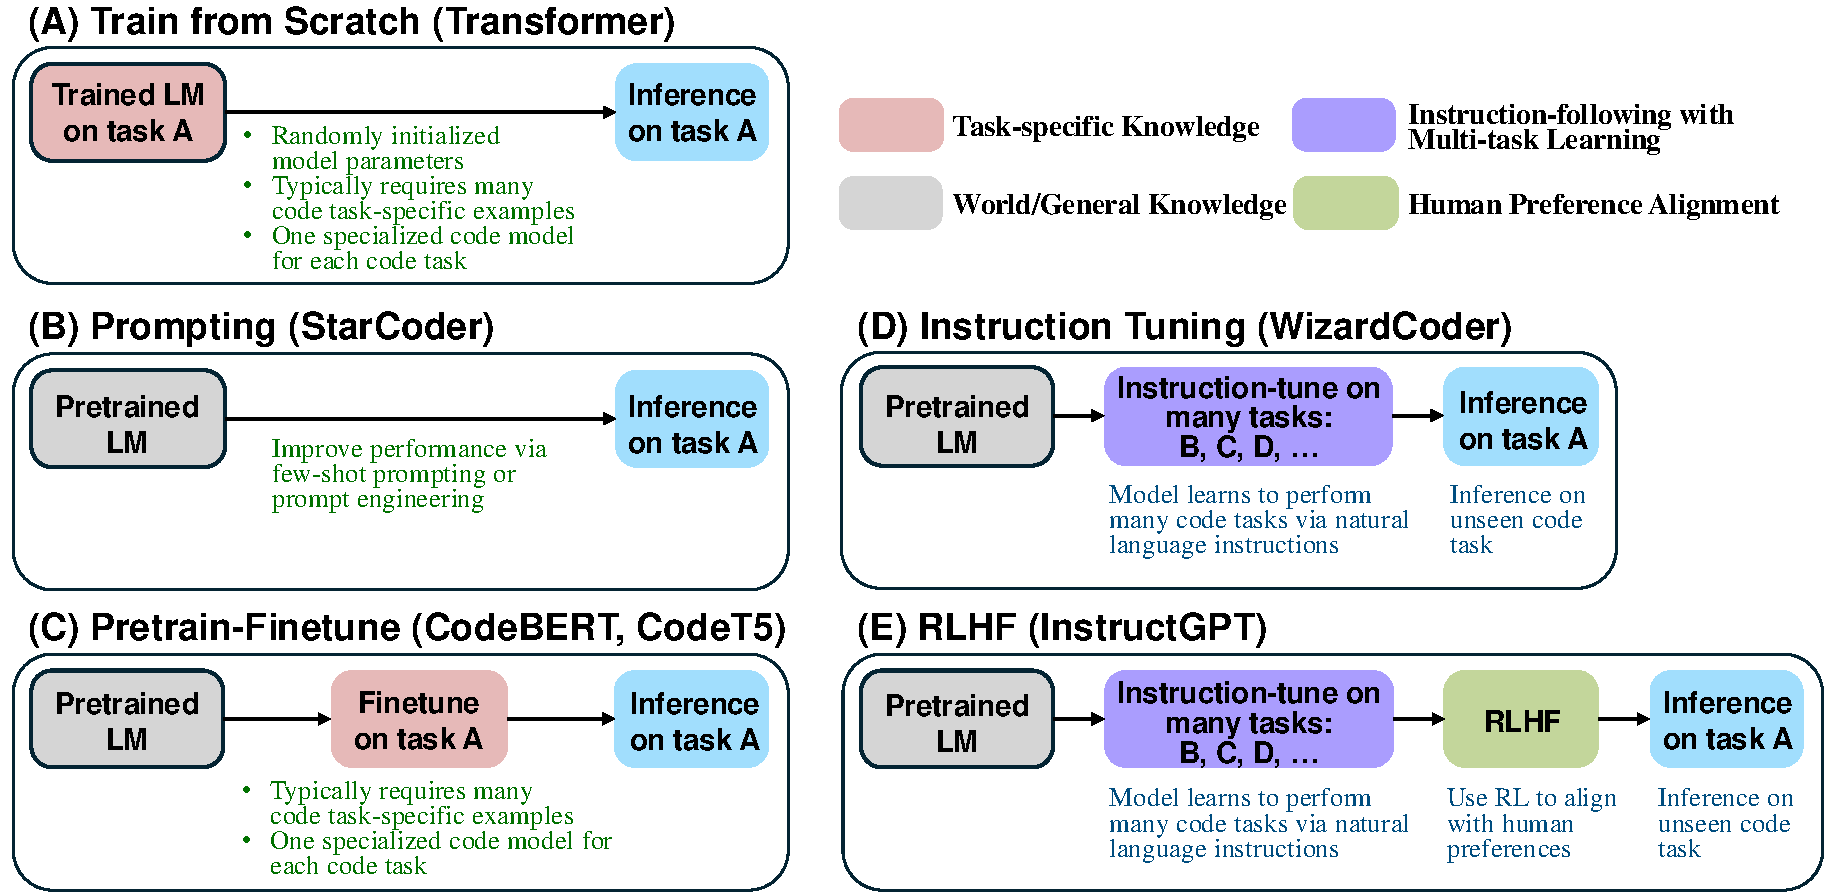
\includegraphics[width=\linewidth]{images/various_ft_v6.pdf}
\caption{\done{Comparison of instruction tuning with various fine-tuning strategies and prompting for code tasks, adapted from \cite{wei2021finetuned}. For (A), which involves training a Transformer from scratch, please refer to \cite{ahmad2020transformer} for its use in source code summarization task. In the case of (E), we utilize a representative RLHF \cite{ouyang2022training} as an example. Additional reinforcement learning methods, such as DPO \cite{rafailov2024direct}, are also applicable at this stage. 
}}
\label{fig:various_ft}
\end{figure*}

\subsection{Instruction Tuning}\label{sec:instruction_tuning}
\begin{figure*}[t]
\centering
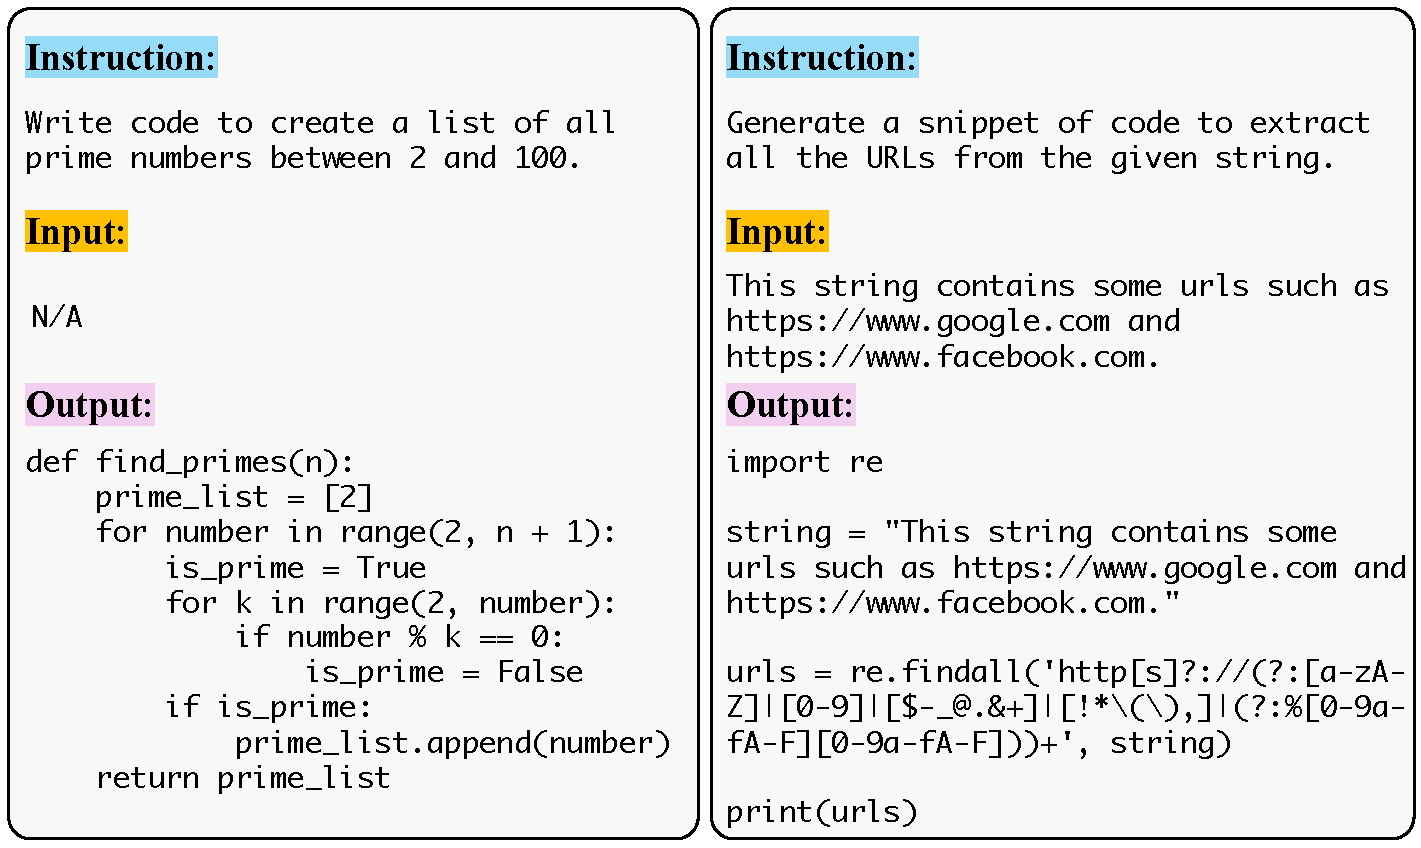
\includegraphics[width=\linewidth]{images/Instruction_Exemplar_v2.pdf}
\caption{Two exemplars of instruction data sampled from Code Alpaca \cite{codealpaca} used to instruction-tune pre-trained code LLM to enhance their alignment with natural language instructions.
The instruction corpus encompasses a variety of tasks, each accompanied by distinct instructions, such as prime numbers generation and URLs extraction.}
\label{fig:instruction}
\end{figure*}

% After pre-training LLM on a large-scale pre-training dataset, in order to endow LLM with the capability to follow instructions, instruction tuning will be performed.
% In general, instruction tuning refers to supervised fine-tuning of pre-trained LLMs on a collection of formatted instances in the form of natural language (instruction) \cite{wei2021finetuned,ouyang2022training,iyer2022opt,zhang2023instruction}. 
% Due to the diversity of instructions, instruction tuning is often regarded as multi-task prompted training, leading to a remarkable generalization ability to unseen tasks \cite{wei2021finetuned,sanh2022multitask,ouyang2022training,chung2024scaling}. 
After pre-training \done{LLMs} on large-scale datasets, the next phase typically involves augmenting the model's ability \done{to process and follow various instructions, known as instruction tuning}. 
\done{Instruction tuning generally refers to the supervised fine-tuning of pre-trained LLMs using datasets comprised of structured examples framed as various natural language instructions \cite{wei2021finetuned,ouyang2022training,iyer2022opt,zhang2023instruction}.
The comparison of instruction tuning with various fine-tuning strategies and prompting for code tasks is depicted in Figure \ref{fig:various_ft}.
} 
Two exemplars of instruction data sampled from Code Alpaca \cite{codealpaca} are demonstrated in Figure \ref{fig:instruction}.
It capitalizes on the heterogeneity of instruction types, positioning instruction tuning as a form of multi-task prompted training that significantly enhances the model's generalization to unseen tasks \cite{wei2021finetuned,sanh2022multitask,ouyang2022training,chung2024scaling}.

% In the code generation, the natural language description can be viewed as an instruction. 
% Therefore, a line of research on instruction tuning LLM for code generation has attracted a lot of attention in academia and industry. 
% In order to perform instruction tuning, instruction data are mainly curated from permissively licensed \cite{husain2019codesearchnet,kocetkov2022stack,lozhkov2024starcoder} (see Section \ref{sec:instruction_data}) or synthetic source code data \cite{luo2023wizardcoder,wei2023magicoder,starcoder2instruct} (see Section \ref{sec:data_synthesis}). 
% Then, these instruction data can be employed to fine-tune LLMs in a supervised learning way.
% However, the inherent large compute resource requirement of large language model constrains the applicability of full parameter fine-tuning LLMs, particularly in resource limit cases \cite{ding2022delta,lialin2023scaling}. 
% In the following subsection, we divide existing works into two categories based on the fine-tuning strategies they use to give a more systematic review.
In the realm of code generation, natural language descriptions serve as the instructions guiding the model to generate corresponding code snippets. 
Consequently, a line of research on instruction tuning LLMs for code generation has garnered substantial interest across academia and industry. 
To perform instruction tuning, instruction data are typically compiled from source code with permissive licenses \cite{husain2019codesearchnet,kocetkov2022stack,lozhkov2024starcoder} (refer to Section \ref{sec:instruction_data}) or are constructed from synthetic code data \cite{luo2023wizardcoder,wei2023magicoder,starcoder2instruct} (refer to Section \ref{sec:data_synthesis}). 
These datasets are then utilized to fine-tune LLMs through a supervised learning paradigm.
However, the substantial computational resources required for full parameter fine-tuning (FFT) LLM pose a notable challenge, particularly in scenarios with constrained resources \cite{ding2022delta,lialin2023scaling}. 
To mitigate this issue, parameter-efficient fine-tuning (PEFT) has emerged as a compelling alternative strategy, gaining increasing attention for its potential to reduce resource consumption \cite{ding2022delta}.
In the following subsection, we categorize existing works based on their instruction-tuning strategies to provide a comprehensive and systematic review.

\subsubsection{Full Parameter Fine-tuning}
% During full parameter fine-tuning (FFT), all parameters of pre-trained models will be updated. When the compute resources and instruction data are sufficient, FFT is a preferred choice because better performance can be achieved.
% \cite{wang2021codet5} proposes a encoder-decoder pre-trained code LLMs termed CodeT5+ and finetunes it on 20K code Alpaca \cite{codealpaca} instruction samples to obtain InstructCodeT5+. 
Full parameter fine-tuning (FFT) involves updating all parameters within a pre-trained model, as shown in Figure \ref{fig:finetune}(a). This approach is often preferred when ample computational resources and substantial training data are available, as it typically leads to better performance.
\cite{wang2021codet5} introduces an encoder-decoder pre-trained language model for code generation, named CodeT5+. They instruction-tune this model on a dataset comprising 20k instruction samples from Code Alpaca \cite{codealpaca}, resulting in an instruction-following model called InstructCodeT5+, which exhibited improved capabilities in code generation.
% WizardCoder \cite{luo2023wizardcoder} utilizes the Evol-Instruct data synthesis technique of WizardLM \cite{xu2023wizardlm} to evolve 20K code Alpaca \cite{codealpaca} instruction samples into a 78K code instruction dataset and then employ it to finetune StarCoder \cite{li2023starcoder} base model.
\cite{luo2023wizardcoder} leverages the Evol-Instruct data synthesis technique from WizardLM \cite{xu2023wizardlm} to evolve 20K code Alpaca \cite{codealpaca} instruction samples into a 78K code instruction dataset. This enriched dataset is then used to fine-tune the StarCoder base model, resulting in WizardCoder, which showcases notable advancements in code generation.
% Inspired by the success of WizardCoder \cite{luo2023wizardcoder} and RRHF \cite{yuan2023rrhf}, Pangu-Coder 2 \cite{shen2023pangu} also uses WizardLM’s Evol-Instruct to generate 68K high-quality instruction samples based on 20K code Alpaca \cite{codealpaca} instruction samples and also proposes a novel reinforcement learning via Rank Responses to align Test \& Teacher Feedback (RRTF) framework to further boost code generation. 
In a similar vein, inspired by the successes of WizardCoder \cite{luo2023wizardcoder} and RRHF \cite{yuan2023rrhf}, Pangu-Coder 2 \cite{shen2023pangu} applies the Evol-Instruct method to generate 68k high-quality instruction samples from the initial 20k Code Alpaca \cite{codealpaca} instruction samples. Additionally, they introduces a novel reinforcement learning via Rank Responses to align Test \& Teacher Feedback (RRTF), which further enhances the performance of Pangu-Coder 2 in code generation.
% Diverging from the above synthetic code instruction data curation, OctoPack \cite{muennighoff2023octopack} uses the natural structure of Git commits, which pair code changes with human instructions to curate CommmitPack which contains 4 terabytes of Git commits across 350 programming languages to instruction tuning StarCoder \cite{li2023starcoder} and CodeGeeX2 \cite{zheng2023codegeex} to obtain OctoCoder and OctoGeeX for code generation, respectively. 
Diverging from synthetic instruction data generation methods, OctoPack \cite{muennighoff2023octopack} utilizes real-world data by curating CommitPack from the natural structure of Git commits, which inherently pair code changes with human-written instructions. 
This dataset, consisting of 4 terabytes of Git commits across 350 programming languages, is employed to fine-tune StarCoder \cite{li2023starcoder} and CodeGeeX2 \cite{zheng2023codegeex}, leading to the instruction-following code models of OctoCoder and OctoGeeX for code generation, respectively.
% Most recently, Magicoder \cite{wei2023magicoder} proposes a novel data synthesis method OSS-INSTRUCT, which enlightens LLMs with open-source code snippets to generate high-quality instruction data for code, aiming to mitigate the inherent bias of the synthetic data generated by LLMs.
% Following the principle of OSS-INSTRUCT proposed by Magicoder, StarCoder2-15B-instruct \cite{starcoder2instruct} released by the BigCode team is claimed as the very first entirely self-aligned code \done{LLM} trained with a fully permissive and transparent pipeline. 
% \cite{codegemma_2024} employs open-source math datasets (e.g., MATH \cite{hendrycks2021measuring} and GSM8k \cite{cobbe2021training}) and synthetically generated code following OSS-Instruct \cite{wei2023magicoder} to instruct tuning CodeGemma 7B, achieving remarkable performance in mathematical reasoning and code generation.
The most recent innovation comes from Magicoder \cite{wei2023magicoder}, who proposes OSS-INSTRUCT, a novel data synthesis method that leverages open-source code snippets to generate high-quality instruction data for code generation. This approach seeks to reduce the bias often present in synthetic data generated by LLM.
In line with OSS-INSTRUCT, the BigCode team introduces StarCoder2-15B-instruct \cite{starcoder2instruct}, which they claim to be the first entirely self-aligned \done{LLM} for code generation, trained with a fully permissive and transparent pipeline.
Moreover, \cite{codegemma_2024} harnesses open-source mathematics datasets, such as MATH \cite{hendrycks2021measuring} and GSM8k \cite{cobbe2021training}, along with synthetically generated code following the OSS-INSTRUCT \cite{wei2023magicoder} paradigm, to instruction-tune CodeGemma 7B, yielding exceptional results in mathematical reasoning and code generation tasks.

\subsubsection{Parameter-Efficient Fine-tuning}\label{sec:peft}
% To reduce the cost and compute resources required for fine-tuning LLM, the principle of parameter-efficient fine-tuning (PEFT) is to only training a small set of parameters which might be a subset of the existing model parameters or a set of newly added parameters \cite{ding2022delta,lialin2023scaling}. 
% A series of novel PEFT methods have been proposed, such as BitFit \cite{zaken2021bitfit}, Adapter \cite{houlsby2019parameter}, Prompt tuning \cite{lester2021power}, Prefix-tuning \cite{li2021prefix}, LoRA \cite{hu2021lora}, IA$^3$ \cite{liu2022few}, QLoRA \cite{dettmers2024qlora}, and AdaLoRA \cite{zhang2023adaptive}.
To mitigate the extensive computational and resource demands inherent in fine-tuning \done{LLMs}, the concept of parameter-efficient fine-tuning (PEFT) has emerged to focus on updating a minimal subset of parameters, which may either be a selection of the model's parameters or an array of additional parameters specifically introduced for the tuning process \cite{ding2022delta,lialin2023scaling}. The categorization of these methods is depicted in Figure \ref{fig:finetune}(b), (c), and (d). 
A plethora of innovative PEFT approaches have been developed, among which BitFit \cite{zaken2021bitfit}, Adapter \cite{houlsby2019parameter}, Prompt tuning \cite{lester2021power}, Prefix-tuning \cite{li2021prefix}, LoRA \cite{hu2021lora}, IA$^3$ \cite{liu2022few}, QLoRA \cite{dettmers2024qlora}, and AdaLoRA \cite{zhang2023adaptive} are particularly noteworthy.
% One of the representative works LoRA \cite{hu2021lora} decomposes parameter update for a pre-trained weight matrix (e.g., the key or value projection matrices in the multi-head self-attention sub-layer of Transformer block) into a product of two low-rank matrices while all pre-trained model parameters are kept frozen, and only two low-rank matrices are trainable. 
% After fine-tuning, the multiplication of two low-rank matrics can be integrated into the original pre-trained weight matrix by element-wise adding operation. Formally,
A seminal study in this field, LoRA \cite{hu2021lora}, proposes a parameter update mechanism for a pre-trained weight matrix — such as those found in the key or value projection matrices of a Transformer block's multi-head self-attention layer — by factorizing the update into two low-rank matrices. Crucially, all original model parameters remain frozen, with only the pair of low-rank matrices being trainable. 
After fine-tuning, the product of these low-rank matrices can be seamlessly incorporated into the existing weight matrix through an element-wise addition. This process can be formally described as:
\begin{equation}
\begin{aligned}
    (\mathbf{W}_0 + \Delta\mathbf{W})x = \mathbf{W}_0x + \Delta\mathbf{W}x = \mathbf{W}_0^{frozen}x + \underbrace{\frac{\alpha}{r}\mathbf{B}^{trainable}_{up}\mathbf{A}^{trainable}_{down}}_{\Delta\mathbf{W}}x
\end{aligned}
\end{equation}
where $\mathbf{W}_0 \in \mathbb{R}^{d\times k}$ denotes a pre-trained weight matrix, $\mathbf{B}^{trainable}_{up} \in \mathbb{R}^{d\times r}$ and $\mathbf{A}^{trainable}_{down} \in \mathbb{R}^{r\times k}$ are two trainable low-rank matrixes and initialized by a zero matrix and a random Gaussian distribution $\mathcal{N}(0,\sigma^{2})$ respectively, to ensure $\Delta\mathbf{W}=0$ at the beginning of training. The rank $r \ll \min(d, k)$, the $\frac{\alpha}{r}$ is a scaling coefficient to balance the importance of the LoRA module, like a learning rate.

% However, there is scarce work adopting PEFT methods into code generation. For example, \cite{codeup} first attempts to parameter-efficient fine-tune a Llama 2 \cite{touvron2023llama2} model on a single RTX 3090 GPU device and proposes a multilingual code generation model namely CodeUp. 
% A more recent work ASTRAIOS \cite{zhuo2024astraios} provides a comprehensive empirical study on parameter-efficient instruction tuning for code understanding and generation tasks, presenting some insightful observations and findings. 
Despite the advancements in PEFT methods, their application in code generation remains limited. For instance, \cite{codeup} pioneered the use of parameter-efficient instruction-tuning on a Llama 2 \cite{touvron2023llama2} model with a single RTX 3090 GPU, leading to the development of a multilingual code generation model called CodeUp. 
More recently, ASTRAIOS \cite{zhuo2024astraios} conducted a thorough empirical examination of parameter-efficient instruction tuning for code comprehension and generation tasks. This study yielded several perceptive observations and conclusions, contributing valuable insights to the domain.

\begin{figure*}[t]
\centering
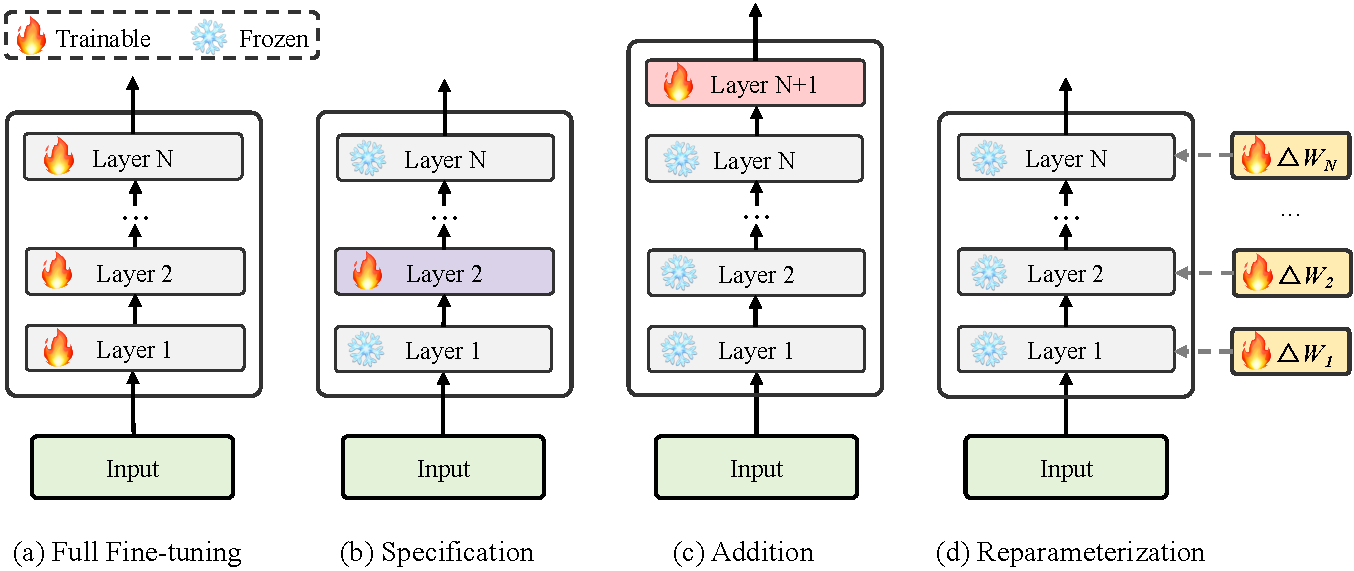
\includegraphics[width=\linewidth]{images/PEFT.pdf}
\caption{An illustration of full parameter fine-tuning (FFT) and parameter-efficient fine-tuning (PEFT) methods.  
(a) refers to the Full Fine-tuning method, which updates all parameters of the base model during fine-tuning. 
(b) stands for the Specification-based PEFT method that conditionally fine-tunes a small subset of the model parameters while freezing the rest of the model, e.g. BitFit \cite{zaken2021bitfit}.
(c) represents the Addition-based PEFT method that fine-tunes the incremental parameters introduced into the base model or input, e.g. Adapter \cite{houlsby2019parameter}, Prefix-tuning
\cite{li2021prefix}, and Prompt-tuning \cite{lester2021power}.
(d) symbolizes the Reparameterization-based method which reparameterizes existing model parameters by low-rank transformation, e.g. LoRA \cite{hu2021lora}, QLoRA \cite{dettmers2024qlora}, and AdaLoRA \cite{zhang2023adaptive}.
}
\label{fig:finetune}
\end{figure*}

%%%%%%%%%%%%%%%%%%%%%%%%%%%%%%%%%%%%%%%%%%%%%%%%%%%%%%%%%%%%%%%%%%%%%%%%
%%%%%%%%%%%%%%%%%%%%%%%%%%%%%%%%%%%%%%%%%%%%%%%%%%%%%%%%%%%%%%%%%%%%%%%%
\subsection{Reinforcement Learning with Feedback}\label{sec:reinforcement_learning}
% DPO and reject sampling
% Despite instruction tuning endows LLM with powerful instruction-following capabilities, large language models can still generate unexpected, toxic, biased content, and hallucinated outputs, which are not aligned with the intention and preference of the user \cite{ouyang2022training,wang2023aligning,ji2023ai}. 
% To this end, aligning LLMs with human expectations has become an active area of interest within the research community. One of the representative works InstructGPT \cite{ouyang2022training} further fine-tunes an instruction-tuned model using reinforcement learning from human feedback (RLHF) on a dataset of labeler-rankings of model outputs from best to worst. 
% Since the RLHF was proposed, it has become one of the key drivers of success in modern conversational language models, such as ChatGPT \cite{gpt-3.5-turbo} and Bard \cite{manyika2023overview}.
% However, gathering high-quality human preference ranking data can be a time-consuming and expensive endeavor \cite{lee2023rlaif}. To mitigate this issue, reinforcement learning from AI Feedback (RLAIF) \cite{bai2022constitutional,lee2023rlaif} is proposed to leverage a powerful off-the-shelf LLM (e.g., ChatGPT \cite{gpt-3.5-turbo} and GPT4 \cite{achiam2023gpt}) to generate preferences in lieu of human annotators.
\done{LLMs} have exhibited remarkable instruction-following capabilities through instruction tuning. However, they often produce outputs that are unexpected, toxic, biased, or hallucinated outputs that do not align with users' intentions or preferences \cite{ouyang2022training,wang2023aligning,ji2023ai}. 
Consequently, aligning LLMs with human preference has emerged as a pivotal area of research. A notable work is InstructGPT \cite{ouyang2022training}, which further fine-tunes an instruction-tuned model utilizing reinforcement learning with human feedback (RLHF) on a dataset where labelers have ranked model outputs in order of quality, from best to worst. 
This method has been instrumental in the development of advanced conversational language models, such as ChatGPT \cite{gpt-3.5-turbo} and Bard \cite{manyika2023overview}.
Despite its success, acquiring high-quality human preference ranking data is a resource-intensive process \cite{lee2023rlaif}. 
To address this, Reinforcement Learning from AI Feedback (RLAIF) \cite{bai2022constitutional,lee2023rlaif} has been proposed to leverage powerful off-the-shelf LLMs (e.g., ChatGPT \cite{gpt-3.5-turbo} and GPT-4 \cite{achiam2023gpt}) to simulate human annotators by generating preference data.

% Inspired by the successful practice of RLHF, researchers have attempted to employ reinforcement learning with feedback to improve the capability of large language models for code generation. 
% However, different from standard RLHF requiring human feedback, compilers or interpreters can be used for automatically generating feedback for code samples generated by large language models. Therefore, it further promotes the rapid development of this line of research.
% CodeRL \cite{le2022coderl} proposes an actor-critic RL framework for code generation, in which code-generating LM is an actor-network and token-level functional correctness reward predictor is a critic. The return reward of generated code is obtained from the unit test signal by a compiler, including compiler error, runtime error, unit test failure, and pass.
% CompCoder \cite{wang2022compilable} utilizes compiler feedback for compilable code generation, including language model fine-tuning, compilability reinforcement, and compilability discrimination to improve the compilability of the generated code.
% Subsequently, PPOCoder \cite{shojaee2023execution} combines pretrained PL model CodeT5 \cite{wang2021codet5} with Proximal Policy Optimization (PPO) \cite{schulman2017proximal} and integrates the execution (compiler) feedback of syntactic or functional correctness, the syntactic and semantic matching scores between the abstract syntax tree (AST) sub-trees and data flow graphs DFG edges of the sampled generations and the ground truth into reward function for model optimization, as well as KL-divergence penalty between active policy and reference pretrained model. 
% More recently, RLTF \cite{liu2023rltf} proposes a novel online RL framework with fine-grained unit test feedback based on the error information and location provided by the compiler, as well as adaptive feedback that takes the ratio of passed test cases into account.
Building on RLHF's success, researchers have explored reinforcement learning with feedback to enhance code generation in LLMs. 
Unlike RLHF, which relies on human feedback, this approach employs compilers or interpreters to automatically provide feedback on code samples through code execution on unit test cases, catalyzing the advancement of this research domain.
CodeRL \cite{le2022coderl} introduced an actor-critic reinforcement learning framework for code generation. In this setup, the language model serves as the actor-network, while a token-level functional correctness reward predictor acts as the critic. Generated code is assessed through unit test signals from a compiler, which can indicate compiler errors, runtime errors, unit test failures, or passes.
CompCoder \cite{wang2022compilable} enhances code compilability by employing compiler feedback, including language model fine-tuning, compilability reinforcement, and compilability discrimination strategies.
Subsequently, PPOCoder \cite{shojaee2023execution} integrates pre-trained code model CodeT5 \cite{wang2021codet5} with Proximal Policy Optimization (PPO) \cite{schulman2017proximal}. This integration not only utilizes execution (\textit{i.e.}, compilers or interpreters) feedback to assess syntactic and functional correctness but also incorporates a reward function that evaluates the syntactic and semantic congruence between abstract syntax tree (AST) sub-trees and data flow graph (DFG) edges in the generated code against the ground truth. 
Additionally, the framework applies a KL-divergence penalty to maintain fidelity between the actively learned policy and the referenced pre-trained model, enhancing the optimization process.
More recently, RLTF \cite{liu2023rltf} has proposed an online reinforcement learning framework that provides fine-grained feedback based on compiler error information and location, along with adaptive feedback that considers the ratio of passed test cases.

% Despite the success, the intrinsic limitations of RL algorithms, such as inefficiency and instability, the vast training resources required, and complex hyper-parameter tuning, hinder the performance and scalability of LLM. 
% To this end, many variants of RL methods without PPO have been proposed recently, such as DPO \cite{rafailov2024direct}, RRHF \cite{yuan2023rrhf}, and sDPO \cite{kim2024sdpo}. 
% In essence, the principle idea of these methods is to maximize the likelihood between the logarithm of conditional probabilities of preferred responses and the logarithm of conditional probabilities of rejected responses. The responses can be generated by the same LLMs or different capabilities of LLMs.
% Inspired by RRHF \cite{yuan2023rrhf}, PanGu-Coder 2 \cite{shen2023pangu} is presented to utilize a novel reinforcement learning via Rank Responses to align Test \& Teacher Feedback (RRTF) framework to further boost code generation, achieving 62.20\% pass@1 on HumanEval benchmark.
Despite these successes, reinforcement learning algorithms face inherent limitations such as inefficiency, instability, extensive resource requirements, and complex hyperparameter tuning, which can impede the performance and scalability of LLMs. 
To overcome these challenges, recent studies have introduced various variants of RL methods that do not rely on PPO, including DPO \cite{rafailov2024direct}, RRHF \cite{yuan2023rrhf}, and sDPO \cite{kim2024sdpo}. 
In essence, these methods aim to maximize the likelihood between the logarithm of conditional probabilities of preferred and rejected responses, which may be produced by LLMs with varying capabilities.
Inspired by RRHF \cite{yuan2023rrhf}, PanGu-Coder 2 \cite{shen2023pangu} leverages a novel framework, Reinforcement Learning via Rank Responses to align Test \& Teacher Feedback (RRTF), significantly enhancing code generation capabilities, as evidenced by \texttt{pass@1} of 62.20\% on the HumanEval benchmark.

% Taking a step forward, more non-differentiable features of code can be integrated into reinforcement learning with feedback of LLM for code generation, such as code style \cite{markovtsev2019style,chen2023duetcs} and readability \cite{buse2009learning}. We expect to see more work in the future. 
Taking a step forward, the integration of more non-differentiable code features, such as coding style \cite{markovtsev2019style,chen2023duetcs} and readability \cite{buse2009learning}, into the reinforcement learning feedback for LLM-based code generation, presents an exciting avenue for future research.

%%%%%%%%%%%%%%%%%%%%%%%%%%%%%%%%%%%%%%%%%%%%%%%%%%%%%%%%%%%%%%%%%%%%%%%%
%%%%%%%%%%%%%%%%%%%%%%%%%%%%%%%%%%%%%%%%%%%%%%%%%%%%%%%%%%%%%%%%%%%%%%%%
\subsection{Prompting Engineering}\label{sec:prompting}
% Large language models trained on a large-scale data corpus already contain a large amount of world knowledge \cite{brown2020language,wei2021finetuned,ouyang2022training}.
% However, how to design a proper prompt to elicit the corresponding capabilities of LLM is a long-standing challenge \cite{liu2023pre}. 
% In recent years, there has been an increasing amount of advanced prompting engineering techniques that allow us to achieve more complex tasks and improve the reliability and performance of LLMs (e.g., ChatGPT and GPT4), such as Chain-of-Thought (CoT) \cite{wei2022chain}, Self-Consistency \cite{wang2022self}, Tree-of-thought (ToT) \cite{yao2024tree}, Reasoning via Planning (RAP) \cite{hao2023reasoning}, ReAct \cite{yao2023react}, Self-Refine \cite{madaan2024self}, Reflexion \cite{shinn2024reflexion}, and LATS \cite{zhou2023language}.
Large-scale language models (LLMs) such as GPT-3 and its successors have been trained on large-scale data corpora, endowing them with substantial world knowledge \cite{brown2020language,wei2021finetuned,ouyang2022training}. 
\done{
Despite this, crafting an effective prompting as a means of communicating with LLMs to harness their full potential remains a long-standing challenge \cite{liu2023pre}.
Recent advancements in prompting engineering have expanded the capabilities of LLMs, enabling more sophisticated task completion and enhancing both reliability and performance.} 
Notable techniques include Chain-of-Thought (CoT) \cite{wei2022chain}, Self-Consistency \cite{wang2022self}, Tree-of-Thought (ToT) \cite{yao2024tree}, Program of Thoughts (PoT) \cite{chen2022program}, Reasoning via Planning (RAP) \cite{hao2023reasoning}, ReAct \cite{yao2023react}, Self-Refine \cite{madaan2024self}, Reflexion \cite{shinn2024reflexion}, and LATS \cite{zhou2023language}.
\done{For instance, CoT significantly improves the LLMs' ability to perform complex reasoning by providing a few chain-of-thought demonstrations as exemplars in prompting.}

% Due to the merit of prompting engineering that does not require extra training and brings significant performance improvement, a series of research has employed feedback for an iterative and self-improved code generation through prompting engineering for powerful proprietary LLMs (e.g., ChatGPT and GPT4).
% For example, Self-Debugging \cite{chen2023teaching} prompts an LLM to iteratively refine its predicted program by employing the feedback message constituted by code explanation along with the execution results of the program to identify its mistakes. When unit tests are not available, the feedback can be purely based on code explanation.
% Similarly, SelfEvolve \cite{jiang2023selfevolve} first prompts LLMs to generate corresponding knowledge for a given problem and then generate the trial code based on the generated knowledge. Subsequently, LLMs are interactively prompted to refine generated code with execution feedback.
Prompting engineering is particularly advantageous as it bypasses the need for additional training and can significantly elevate performance. 
\done{Consequently, numerous studies have leveraged this technique for iterative and self-improving (refining) code generation within proprietary LLMs such as ChatGPT and GPT-4.} 
Figure \ref{fig:reflection} illustrates the general pipeline for self-improving code generation with LLMs.
For instance, Self-Debugging \cite{chen2023teaching} involves prompting an LLM to iteratively refine a predicted program by utilizing feedback composed of code explanations combined with execution results, which assists in identifying and rectifying errors. 
When unit tests are unavailable, this feedback can rely solely on code explanations. 
\done{
Similarly, LDB \cite{zhong2024ldb} prompts LLMs to refine generated code by incorporating debugging feedback, which consists of the evaluation of the correctness of variable values throughout runtime execution, as assessed by the LLMs.
}
In parallel, SelfEvolve \cite{jiang2023selfevolve} employs a two-stage process where LLMs first generate domain-specific knowledge for a problem, followed by a trial code. This code is then iteratively refined through interactive prompting and execution feedback.
% To provide an in-depth understanding of self-refinement for code generation through prompting, \cite{olausson2023self} conducts an empirical study to analyze Code Llama, GPT-3.5 and GPT-4’s ability to perform self-repair (debug) on problems taken from HumanEval and APPS, and draws some insightful observation and findings. 
% Furthermore, a more general approach Reflexion \cite{shinn2024reflexion} prompts LLM-powered agents to verbally self-reflect on task feedback signals, then maintain their own reflective text in an episodic memory buffer to induce better decision-making in subsequent trials (actions).
An empirical investigation by \cite{olausson2023self} provides a comprehensive analysis of the self-repairing capabilities for code generation in models like Code Llama, GPT-3.5, and GPT-4, using problem sets from HumanEval and APPS. This study yields a series of insightful observations and findings, shedding light on the self-refinement effectiveness of these LLMs.
Moreover, Reflexion \cite{shinn2024reflexion} introduces a general approach for code generation wherein LLM-powered agents engage in verbal self-reflection on task feedback signals, storing these reflections in an episodic memory buffer to inform and improve decision-making in subsequent interactions.
% LATS \cite{zhou2023language} employs LLMs as agents, value functions, and optimizers to enhance decision-making by deliberately constructing trajectories with Monte Carlo Tree Search (MCTS)-based search algorithms, incorporating external feedback, and enabling agents to learn from experience, achieving an impressive 94.4\% on HumanEval benchmark with GPT-4.
LATS \cite{zhou2023language} adopts a novel strategy, utilizing LLMs as agents, value functions, and optimizers. It enhances decision-making by meticulously constructing trajectories through Monte Carlo Tree Search (MCTS) algorithms, integrating external feedback, and learning from experience. 
This approach has demonstrated remarkable results in code generation, achieving a \texttt{pass@1} of 94.4\% on the HumanEval benchmark with GPT-4.

\begin{figure*}[t]
\centering
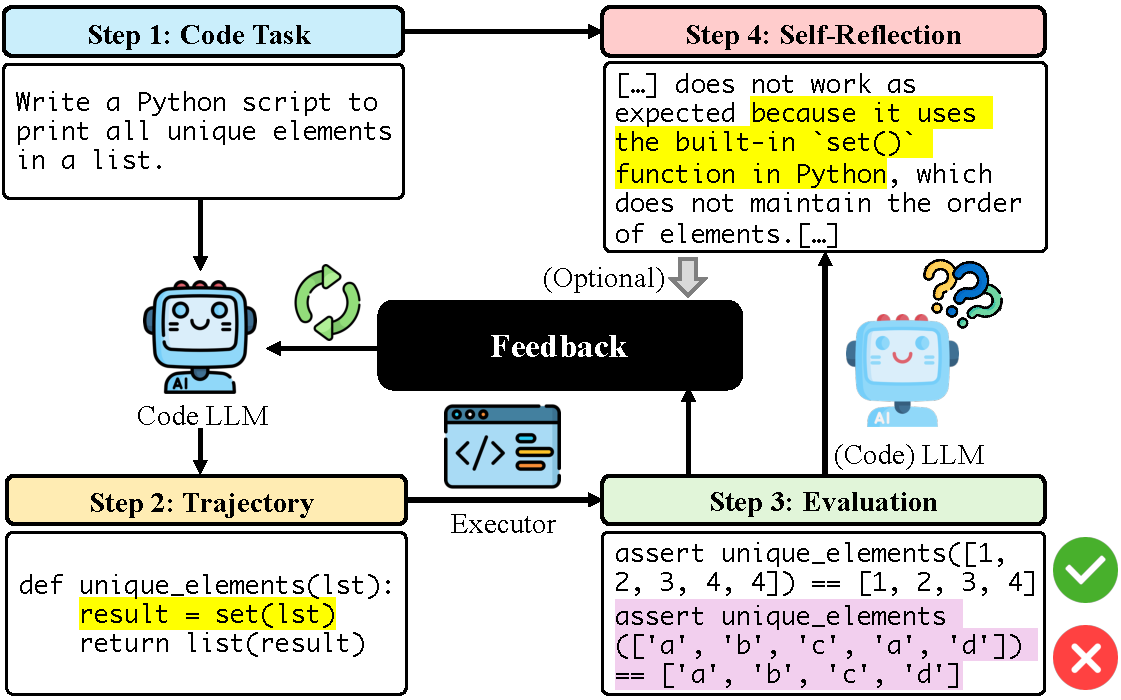
\includegraphics[width=0.95\linewidth]{images/Self-Refine_v6.pdf}
\caption{An illustration of the self-improving code generation pipeline using prompts for \done{LLMs}. This process incorporates iterative self-refinement by integrating execution outcomes and includes an optional self-reflection mechanism to enhance generation quality.
% The pipeline of prompting LLM to self-refine code generation with feedback constituted by execution results and self-reflection (optional).
}
\label{fig:reflection}
\end{figure*}
% In particular, CodeT \cite{chen2022codet} and LEVER \cite{ni2023lever} prompt LLM to generate a lot of samples and then re-rank them based on execution results to obtain the best code solution while both do not implement a self-refinement step to improve code writing.
Distinct from the aforementioned methods, CodeT \cite{chen2022codet} and LEVER \cite{ni2023lever} prompt LLMs to generate numerous code samples, which are then re-ranked based on execution outcomes to select the optimal solution. Notably, these approaches do not incorporate a self-refinement step to further improve code generation.

%%%%%%%%%%%%%%%%%%%%%%%%%%%%%%%%%%%%%%%%%%%%%%%%%%%%%%%%%%%%%%%%%%%%%%%%
%%%%%%%%%%%%%%%%%%%%%%%%%%%%%%%%%%%%%%%%%%%%%%%%%%%%%%%%%%%%%%%%%%%%%%%%
\subsection{Repository Level \& Long Context}\label{sec:repository_level}
% In real-world software engineering activities, it involves pervasively editing the entire repository of code, such as package migration, temporal code edits, and GitHub issues fixing. 
% Despite the remarkable capabilities of large language models for code generation, LLMs struggle to understand a broader context present in the repository, such as imports, parent classes, and files with similar names, leading to significantly poor performance in repository-level code generation \cite{shrivastava2023repository,shrivastava2023repofusion}. 
% The reason behind the failure is mainly attributed to the following points:
% 1) Code within a repository has broader and more complex inter-dependencies scatted in different code files, such as shared utilities, configurations, and cross-API invocations caused by modularization \cite{zhang2023repocoder,bairi2023codeplan}.
% 2) Each repository has its unique structure, naming conventions, and coding style to ensure clear readability and maintainability \cite{chen2023duetcs}.
% 3) Taking the context from the entire repository may be too large to fit into the prompt due to the context length limitation of LLMs \cite{bairi2023codeplan}. 
% 4) LLMs are not fully trained on a large number of repository data, such as proprietary software or work-in-progress code projects \cite{shrivastava2023repofusion}.
In contemporary software engineering practices, modifications to a code repository are widespread and encompass a range of activities, including package migration, temporary code edits, and the resolution of GitHub issues. 
While \done{LLMs} showcase impressive prowess in function-level code generation, they often falter when grappling with the broader context inherent to a repository, such as import dependencies, parent classes, and files bearing similar names. 
These deficiencies result in suboptimal performance in repository-level code generation, as identified in recent studies \cite{shrivastava2023repository,shrivastava2023repofusion}.
The challenges faced by LLMs in this domain are primarily due to the following factors:
\begin{itemize}
    \item Code repositories typically contain intricate interdependencies scattered across various files, including shared utilities, configurations, and cross-API invocations, which arise from modular design principles \cite{zhang2023repocoder,bairi2023codeplan}.
    \item Repositories are characterized by their unique structures, naming conventions, and coding styles, which are essential for maintaining clarity and facilitating ongoing maintenance \cite{chen2023duetcs}.
    \item The vast context of an entire repository often exceeds the context length limitations of LLMs, thus hindering their ability to integrate comprehensive contextual information \cite{bairi2023codeplan}.
    \item LLMs may not have been adequately trained on extensive sets of repository data, such as proprietary software or projects that are still in development \cite{shrivastava2023repofusion}.
\end{itemize}

% In a practical software development scenario, the scale of the repository generally involves hundreds of thousands of tokens. Thus, it is essential to enhance the capability of the long context of LLMs when we adopt LLM for repository-level code generation. Fortunately, a plethora of positional-encoding-based methods have been proposed to enhance length extrapolation (generalizing from short training sequences to longer inference ones) of Transformer \cite{zhao2023length}, such as ALiBi \cite{press2021train} and RoPE \cite{su2024roformer}. It mitigates the third issue in above mentioned reasons to some extent, making it possible to contextualize coding activities within entire repositories.
Given that the scope of a typical software repository encompasses hundreds of thousands of tokens, it is imperative to enhance the capacity of LLMs to handle extensive contexts when they are employed for repository-level code generation. Fortunately, recent advancements in positional encoding techniques, such as ALiBi \cite{press2021train} and RoPE \cite{su2024roformer}, have shown promise in improving the Transformer's ability to generalize from shorter training sequences to longer inference sequences \cite{zhao2023length}. This progress addresses the third challenge mentioned above to a certain degree, thereby enabling better contextualization of coding activities within full repositories.

% To further enhance the capabilities of LLM for repository-level code completion, RepoCoder \cite{zhang2023repocoder} utilizes a similarity-based retriever to select the relevant context of the repository with an iterative retrieval-generation paradigm to enhance the quality of retrieval context and code completion. 
% Similarly, CoCoMIC \cite{ding2022cocomic} utilizes a cross-file context finder CCFINDER to locate and retrieve the most relevant cross-file context in the repository, while RepoHyper \cite{phan2024repohyper} first employs a semantic graph structure namely RSG to encapsulate the vast context of code repositories and then leverages a Expand and Refine retrieval method to retrieve relevant code snippets. 
% \cite{shrivastava2023repository} propose RLPG framework to generate repository-level prompt, which incorporates both the structure of the repository as well as the relevant context in all the files of the repository. 
% However, the invariable use of retrieval exposes issues in both efficiency and robustness as some retrieved contexts are unhelpful or harmful.
% To this end, \cite{wu2024repoformer} proposes a selective RAG framework termed Repoformer where retrieval is avoided when unnecessary. To be specific, they design a self-supervised learning approach that enables a code LM to accurately self-evaluate whether retrieval can improve its output quality and robustly leverage the potentially noisy retrieved contexts.
To further refine LLMs for repository-level code completion, several innovative approaches have been introduced. 
RepoCoder \cite{zhang2023repocoder} leverages a similarity-based retrieval system within an iterative retrieval-generation paradigm to enrich the context and enhance code completion quality. 
In a similar vein, CoCoMIC \cite{ding2022cocomic} employs a cross-file context finder named CCFINDER to pinpoint and retrieve the most relevant cross-file contexts within a repository. 
RepoHyper \cite{phan2024repohyper} introduces a semantic graph structure, termed RSG, to encapsulate the expansive context of code repositories and uses an ``Expand and Refine'' retrieval method to obtain relevant code snippets. 
Moreover, a framework known as RLPG \cite{shrivastava2023repository} has been proposed to generate repository-level prompts that integrate the repository's structure with the relevant context across all files. 
However, the constant reliance on retrieval mechanisms has raised concerns regarding efficiency and robustness, as some retrieved contexts may prove unhelpful or harmful. In response, Repoformer \cite{wu2024repoformer} introduces a selective Retrieval-Augmented Generation (RAG) framework that judiciously bypasses retrieval when it is deemed redundant. This approach incorporates a self-supervised learning strategy that equips a code LLM with the ability to perform a self-assessment on the utility of retrieval for enhancing the quality of its output, thereby effectively utilizing potentially noisy retrieved contexts.

% Furthermore, different from retrieving relevant context to enhance inference, RepoFusion \cite{shrivastava2023repofusion} is proposed to train models to combine multiple relevant contexts from the repository to generate more accurate and context-aware code completions. 
% More recently, Microsoft presented an LLM-powered agent namely CodePlan \cite{bairi2023codeplan} which frames repository-level coding tasks as a planning problem. To be specific, it synthesizes a multi-step chain of edits (plan), where each step results in a call to an LLM on a code location with context derived from the entire repository, previous code changes, and task-specific instructions. 
Additionally, RepoFusion \cite{shrivastava2023repofusion} has been developed to train models to combine multiple relevant contexts from a repository, aiming to produce more precise and context-aware code completions. 
In a novel approach, Microsoft's CodePlan \cite{bairi2023codeplan} frames repository-level coding tasks as a planning problem, generating a multi-step chain of edits (plan) where each step involves invoking an LLM on a specific code location, considering context from the entire repository, preceding code modifications, and task-specific instructions.

% Taking one more step forward, \cite{zan2024codes} first delves into the much harder task of NL2Repo, which generates an entire code repository from its natural language requirements, and proposes CodeS framework to decompose NL2Repo into multiple sub-tasks by a multi-layer sketch. 
% Specifically, CodeS is composed of three modules: 1) RepoSketcher for generating a repository’s directory structure for given requirements, 2) FileSketcher for generating a file sketch for each file in the generated structure, and 3) SketchFiller for generating the details for each function in the generated file sketch.
% Taking one more step forward, \cite{zan2024codes} first delves into a much harder task termed NL2Repo, which involves generating a complete code repository from its natural language requirements, and proposes CodeS framework breaks down NL2Repo into multiple sub-tasks using a multi-layer sketch. 
% This framework consists of three core components: 1) RepoSketcher, for creating a directory structure based on given requirements; 2) FileSketcher, for sketching out each file within that structure; and 3) SketchFiller, for fleshing out the specifics of each function within the file sketches \cite{zan2024codes}.
Advancing the state-of-the-art, \cite{zan2024codes} tackles the formidable challenge of NL2Repo, an endeavor that seeks to create a complete code repository from natural language requirements. To address this complex task, they introduce the CodeS framework, which strategically breaks down NL2Repo into a series of manageable sub-tasks using a multi-layer sketch approach. The CodeS framework comprises three distinct modules: 
1) RepoSketcher, for creating a directory structure of the repository based on given requirements; 
2) FileSketcher, for sketching out each file within that structure; and 
3) SketchFiller, for fleshing out the specifics of each function within the file sketches \cite{zan2024codes}.

% Accordingly, an increasing number of benchmarks for repository-level code generation are also proposed, such as RepoEval \cite{zhang2023repocoder}, Stack-Repo \cite{shrivastava2023repofusion}, Repobench \cite{liu2023repobench}, EvoCodeBench \cite{li2024evocodebench}, SWE-bench \cite{jimenez2023swe}, CrossCodeEval \cite{ding2024crosscodeeval}, and SketchEval \cite{zan2024codes}.
Accordingly, a surge of benchmarks tailored for repository-level code generation has emerged, such as RepoEval \cite{zhang2023repocoder}, Stack-Repo \cite{shrivastava2023repofusion}, Repobench \cite{liu2023repobench}, EvoCodeBench \cite{li2024evocodebench}, SWE-bench \cite{jimenez2023swe}, CrossCodeEval \cite{ding2024crosscodeeval}, and SketchEval \cite{zan2024codes}. The detailed statistics and comparisons of these benchmarks are presented in Table \ref{tab:benchmark}.

% Although the above methods have made some progress in repository-level code generation, they still suffer from requiring programming developers to spend a lot of time editing and debugging \cite{vaithilingam2022expectation,mozannar2022reading,shrivastava2023repofusion,barke2023grounded,bird2022taking}.
% Recently, LLM-powered agents for code (see more details in Section \ref{sec:autonomous_agents}), such as AutoCodeRover \cite{zhang2024autocoderover}, SWE-Agent \cite{swe-agent}, and OpenDevin \cite{OpenDevin}, have been demonstrated a great potential to solve complex problems, opening up exciting avenues for future research in repository-level code generation.
Despite the progress made by these methods in repository-level code generation, significant challenges remain to be addressed. Programming developers are often required to invest considerable time in editing and debugging \cite{vaithilingam2022expectation,mozannar2022reading,shrivastava2023repofusion,barke2023grounded,bird2022taking}. However, the advent of LLM-powered coding agents, such as AutoCodeRover \cite{zhang2024autocoderover}, SWE-Agent \cite{swe-agent}, and OpenDevin \cite{OpenDevin}, has demonstrated their potential to tackle complex problems, paving the way for future exploration in this field (for more details, see Section \ref{sec:autonomous_agents}).

%提一下长度可以处理了,由于long context的技术
%随后介绍各个工作的具体做法
%agent的工作系列提一下
%benchmarks
%展望未来
% involve pervasively editing the entire repository of code
% has shown the promise of using context from the repository during inference
% based on a broader context of the repository.
% Introducing domain-specific knowledge in the prompt design process becomes important.
% take context from the entire repository,
% incorporating both the structure of the repository and the context from other relevant files (e.g. imports, parent class files).

% Most tasks discussed in Section 2.1 are limited to a single file or even a single function, as cross-file code modeling poses challenges that are beyond the capability of most existing language models. Recently, however, position interpolation techniques (Chen et al., 2023b; Rozière et al., 2023; Peng et al., 2023a) have extended the context window of LLMs to hundreds of thousands of tokens, making it possible to contextualize coding activities within entire repositories. Several works have studied code completion (Shrivastava et al., 2023b; Ding et al., 2022b; Zhang et al., 2023b; Shrivastava et al., 2023a; Phan et al., 2024; Wu et al., 2024) and generation (Liao et al., 2023; Zan et al., 2024) leveraging repository-level context, and corresponding benchmarks have been proposed Liu et al. (2023j); Ding et al. (2023); Li et al. (2024a). Bairi et al. (2023) investigate the more challenging tasks of repository-level API migration and temporal editing, while Jimenez et al. (2023) introduce a related benchmark, SWE-bench.

%%%%%%%%%%%%%%%%%%%%%%%%%%%%%%%%%%%%%%%%%%%%%%%%%%%%%%%%%%%%%%%%%%%%%%%%
%%%%%%%%%%%%%%%%%%%%%%%%%%%%%%%%%%%%%%%%%%%%%%%%%%%%%%%%%%%%%%%%%%%%%%%%
\subsection{Retrieval Augmented}\label{sec:retrieval_augmented}
\begin{figure*}[t]
\centering
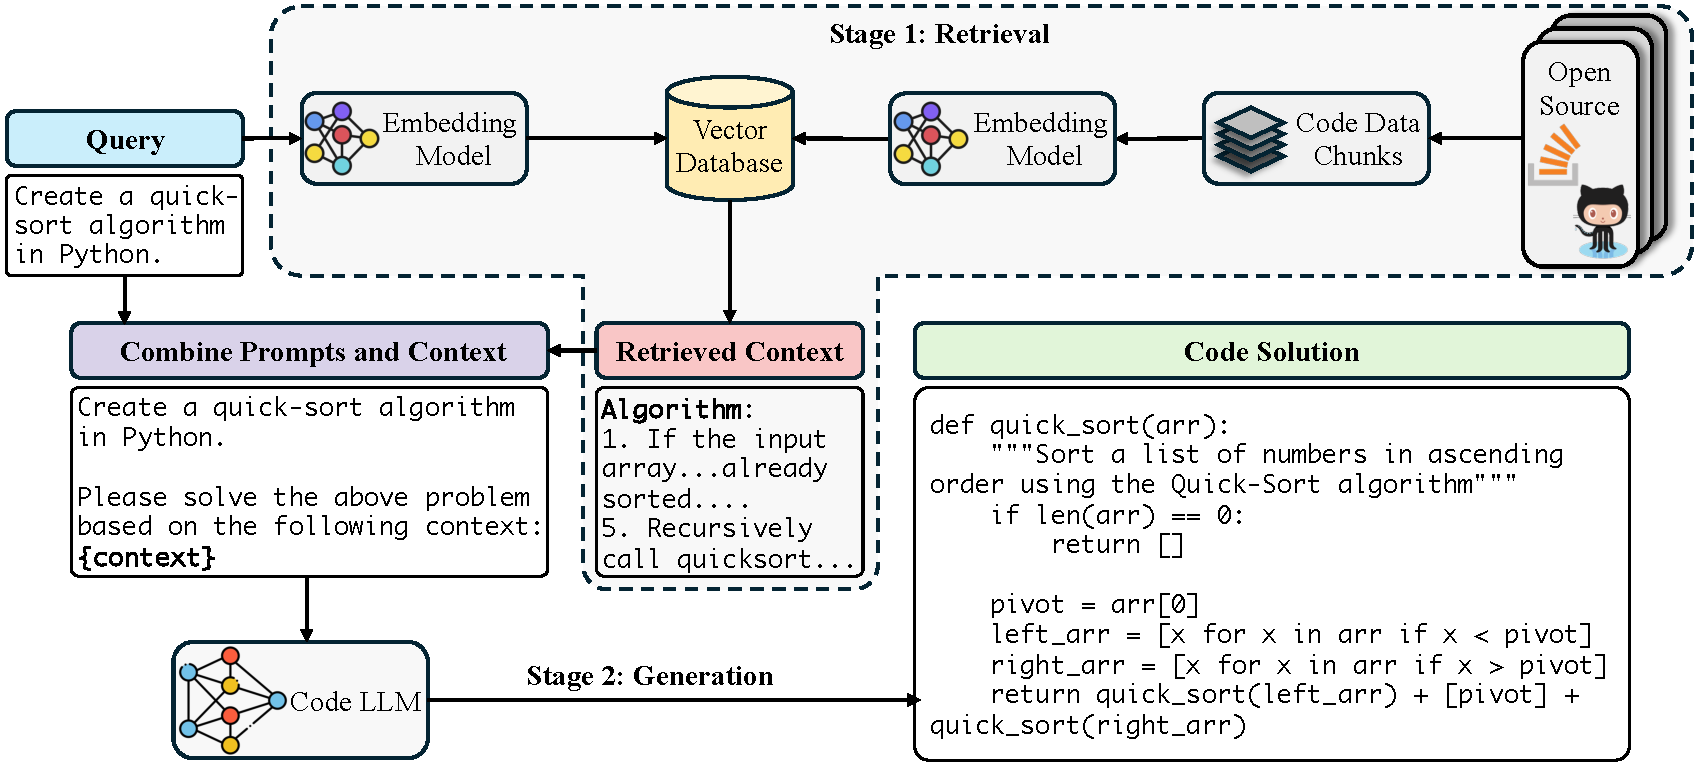
\includegraphics[width=\linewidth]{images/RAG_Code_v4.pdf}
\caption{A workflow illustration of the Retrieval-Augmented Code Generation (RACG). Upon receiving a query (instruction), the retriever selects the relevant contexts from a large-scale vector database. Subsequently, the retrieved contexts are merged with the query, and this combined input is fed into the generator (LLM) to produce the target code solution.
% A pipeline illustration of RAG for code generation. Given a query (instruction), the retriever first retrieves top-k candidate code from a large-scale vector database. Then, the retrieved context is combined with the query and taken that as input for the generator (LLM) to generate the target code.
}
\label{fig:rag}
\end{figure*}
% these researchers showcase the prowess of LLMs in generating accurate API calls and adapting to real-time documentation changes, effectively addressing challenges like hallucination and inaccurate input arguments.
% \done{LLMs} have demonstrated remarkable capabilities but still suffer from crucial challenges like hallucination \cite{liang2023holistic,zhang2023siren}, outdated knowledge \cite{jang2022towards}, and non-transparent \cite{bommasani2021opportunities}, untraceable reasoning processes \cite{zhou2022least,wei2022chain,huang2023towards,gao2023retrieval}.
% Although the above-mentioned instruction-tuning (see Section \ref{sec:instruction_tuning}) and reinforcement learning with feedback (see Section \ref{sec:reinforcement_learning}) eliminate these challenges, they are still facing the catastrophic forgetting and intensive computing resources required for training \cite{ovadia2023fine,gupta2024rag}.
\done{LLMs} have exhibited impressive capabilities but are hindered by several critical issues such as hallucination \cite{liang2023holistic,zhang2023siren}, obsolescence of knowledge \cite{jang2022towards}, and non-transparent \cite{bommasani2021opportunities}, untraceable reasoning processes \cite{zhou2022least,wei2022chain,huang2023towards,gao2023retrieval}. 
While techniques like instruction-tuning (see Section \ref{sec:instruction_tuning}) and reinforcement learning with feedback (see Section \ref{sec:reinforcement_learning}) mitigate these issues, they also introduce new challenges, such as catastrophic forgetting and the requirement for substantial computational resources during training \cite{ovadia2023fine,gupta2024rag}.

% Recently, Retrieval-Augmented Generation (RAG) has emerged as a promising solution to address these challenges by incorporating retrieved knowledge from external databases. 
% Formally, the specific definition of RAG refers to the model, when answering questions or generating text or code, first retrieving relevant information from a vast corpus of documents. Subsequently, it utilizes this retrieved information as more context with an original query to generate responses or text, thereby enhancing the quality and credibility of generation, particularly for knowledge-intensive tasks. 
% In general, the RAG framework is composed of a vector database, retriever, re-ranker, and generator. In practice, it is often implemented by LangChain\footnote{LangChain gives developers a framework to construct LLM‑powered applications easily. \href{https://www.langchain.com}{https://www.langchain.com}} and LLamaIndex\footnote{LlamaIndex is the leading data framework for building LLM applications. \href{https://www.llamaindex.ai/}{https://www.llamaindex.ai}}. 
% RAG allows for continuous knowledge updates and integration of domain-specific information for LLM without training from scratch \cite{gao2023retrieval}. Therefore, RAG has substantially improved the LLM performance across a variety of tasks \cite{lewis2020retrieval,chen2024benchmarking}.  
Recently, Retrieval-Augmented Generation (RAG) has emerged as an innovative approach to overcoming these limitations by integrating knowledge from external databases. Formally defined, RAG denotes a model that, in response to queries, initially sources relevant information from an extensive corpus of documents, and then leverages this retrieved information in conjunction with the original query to enhance the response's quality and accuracy, especially for knowledge-intensive tasks. 
The RAG framework typically consists of a vector database, a retriever, a re-ranker, and a generator. 
It is commonly implemented using tools such as LangChain\footnote{LangChain facilitates the development of LLM-powered applications. \href{https://www.langchain.com}{https://www.langchain.com}} and LLamaIndex\footnote{LLamaIndex is a leading data framework for building LLM applications. \href{https://www.llamaindex.ai/}{https://www.llamaindex.ai}}. 
By performing continuous knowledge updates of the database and the incorporation of domain-specific data, RAG circumvents the need for re-training LLMs from scratch \cite{gao2023retrieval}. Consequently, RAG has substantially advanced LLM performance across a variety of tasks \cite{lewis2020retrieval,chen2024benchmarking}.

% Due to the nature of code, code LLMs also suffer from the above challenges for general-purpose LLMs. 
% For example, it will result in a hallucination phenomenon when the instruction is beyond the code training data or requires the latest released programming package. 
% In particular, publicly available source-code libraries (e.g., PyTorch) are constantly growing and updating, leading to some calling methods being deprecated. 
% Thus, if the Code LLMs are not updated along with all available functions and APIs, it will raise some potential errors and risks. 
% Fortunately, it is promising to call for retrieval augmented code generation to address these challenges. The principle pipeline of RAG for code generation is illustrated in Figure \ref{fig:rag}.
Due to the nature of code, code LLMs are also susceptible to the aforementioned issues that affect general-purpose LLMs. 
For instance, they may exhibit a hallucination phenomenon when instructions fall outside the scope of their training data or necessitate the latest programming packages. 
Given the dynamic nature of publicly available source-code libraries like PyTorch, which undergo frequent expansion and updates, deprecated calling methods can become a significant challenge. 
If Code LLMs are not updated in tandem with the latest functions and APIs, this can introduce potential errors and safety risks. 
Retrieval-Augmented Code Generation (RACG) stands as a promising solution to these concerns. A workflow illustration of the RACG is depicted in Figure \ref{fig:rag}.

% Nevertheless, there are scarce works that have adopted RAG for code generation. 
% Inspired by human behaviors of copying from the related code snippets when writing code, \cite{liu2020retrieval} proposes a novel retrieval-augmented mechanism with graph neural networks (GNNs) termed HGNN to combine the benefits of retrieving similar examples and better generalization capability of the generation-based model for code summarization, which is an inverse operation of code generation. 
% \cite{parvez2021retrieval} first attempt to propose a retrieval augmented framework named REDCODER for code generation tasks through retrieving relevant code from a retrieval database and providing them as a supplement to code generation models. 
% Subsequently, a retrieval-augmented code completion framework termed ReACC \cite{lu2022reacc} is proposed to leverage both lexical copying and referring to code with similar semantics by retrieval and achieves a state-of-the-art performance on CodeXGLUE benchmark \cite{lu2021codexglue}.
% Inspired by human programmers frequently refer to textual resources such as code manuals and documentation to explore and understand the available functionality,
% DocPrompting \cite{zhou2022docprompting} explicitly leverages code documentation by retrieving the relevant documentation pieces given a natural language (NL) intent (query) and generating target code based on the NL intent and the retrieved documentation.
% More recently, an iterative retrieval-generation framework for repository-level code completion termed RepoCoder \cite{zhang2023repocoder} is proposed to achieve the usage of similar code information across different files in the repository. 
% Moreover, to break the dependence on a single retrieval source, \cite{su2024arks} constructs a knowledge soup integrating web search, documentation, execution feedback, and evolved code snippets and employs an active retrieval strategy that iteratively refines the query and updates the knowledge soup. 
Despite its potential, the adoption of RAG for code generation remains limited. 
Drawing inspiration from the common practice among programmers of referencing related code snippets, \cite{liu2020retrieval} introduced a novel retrieval-augmented mechanism with graph neural networks (GNNs), termed HGNN, which unites the advantages of similar examples retrieval with the generalization capabilities of generative models for code summarization, which is the reverse process of code generation.
\cite{parvez2021retrieval} pioneered a retrieval augmented framework named REDCODER for code generation by retrieving and integrating relevant code snippets from a source-code database, thereby providing supplementary context for the generation process. 
Subsequently, a retrieval-augmented code completion framework termed ReACC \cite{lu2022reacc} is proposed to leverage both lexical copying and semantic referencing of related code, achieving state-of-the-art performance on the CodeXGLUE benchmark \cite{lu2021codexglue}.
In the spirit of how programmers often consult textual resources such as code manuals and documentation to comprehend functionalities, DocPrompting \cite{zhou2022docprompting} explicitly utilizes code documentation by retrieving the relevant documentation pieces based on a natural language query and then generating the target code by blending the query with the retrieved information.

More recently, RepoCoder \cite{zhang2023repocoder}, an iterative retrieval-generation framework, is proposed for enhancing repository-level code completion by effectively utilizing code analogies across different files within a repository to inform and improve code suggestions.
Furthermore, breaking away from reliance on a singular source of retrieval, \cite{su2024arks} developed a multi-faceted ``knowledge soup'' that integrates web searches, documentation, execution feedback, and evolved code snippets. Then, it incorporates an active retrieval strategy that iteratively refines the query and enriches the knowledge soup, expanding the scope of information available for code generation.

% Despite these advantages, there are still some potential limitations for retrieval augmented code generation that need to be addressed in the future: 1) the quality of retrieval information will significantly affect the final performance; 2) how to effectively integrate retrieval code information and query (instruction); 3) the quality of response may be still poor or worse, due to over-reliance on retrieval information to ignore query intent; 4) the retrieval information increases the length of the context, requiring a larger context window for the LLM and more compute resources. 
Despite these advancements, several limitations in retrieval-augmented code generation warrant further exploration: 1) the quality of the retrieved information significantly impacts overall performance; 2) the effective integration of retrieved code information with the query needs optimization; 3) an over-reliance on retrieved information may lead to inadequate responses that fail to address the query's intent; 4) additional retrieved information necessitates larger context windows for the LLM, resulting in increased computational demands.

%%%%%%%%%%%%%%%%%%%%%%%%%%%%%%%%%%%%%%%%%%%%%%%%%%%%%%%%%%%%%%%%%%%%%%%%
%%%%%%%%%%%%%%%%%%%%%%%%%%%%%%%%%%%%%%%%%%%%%%%%%%%%%%%%%%%%%%%%%%%%%%%%
\subsection{Autonomous Coding Agents}\label{sec:autonomous_agents}
% AutoGPT, AutoGen, CS list table, OpenInterpreter
% Due to the powerful capabilities of large language models, LLM-powered autonomous agents have emerged as a promising pathway towards artificial general intelligence (AGI) and gained tremendous interest in both industry and academia \cite{xi2023rise,weng2023agent,wang2024survey,huang2024position}. 
% A burgeoning LLM-based autonomous agents applications have emerged rapidly, such as AutoGPT \cite{autogpt}, AgentGPT \cite{agentgpt}, BabyAGI \cite{babyagi}, and AutoGen \cite{wu2023autogen}.
The advent of \done{LLMs} has marked the beginning of a new era of
% has ushered in a new era of 
potential pathways toward artificial general intelligence (AGI), capturing significant attention in both academia and industry \cite{xi2023rise,weng2023agent,wang2024survey,huang2024position}. 
A rapidly expanding array of applications for LLM-based autonomous agents, including AutoGPT \cite{autogpt}, AgentGPT \cite{agentgpt}, BabyAGI \cite{babyagi}, and AutoGen \cite{wu2023autogen}, underlines the promise of this technology.

% Formally, LLM-powered agents are described as a system with complex reasoning capabilities that can use an LLM as its core computational engine (also termed controller) to reason through a problem, create a plan to solve the problem and execute the plan with a set of tools (functions/APIs calling). 
% Besides, agents operate in a shared environment and can communicate, cooperate, compete, or negotiate with each other \cite{huang2023agentcoder,wu2023autogen,wang2024survey}. 
% In general, an LLM-powered autonomous agent is composed of an Agent (LLM), memory module, planning module, and tool use, as shown in Figure \ref{fig:agent}. 
LLM-powered autonomous agents are systems endowed with sophisticated reasoning abilities, leveraging an LLM as a central computational engine or controller. This allows them to formulate and execute problem-solving plans through a series of tool-enabled functions or API calls. 
Moreover, these agents are designed to function within a shared environment where they can communicate and engage in cooperative, competitive, or negotiating interactions \cite{huang2023agentcoder,wu2023autogen,wang2024survey}. 
The typical architecture of such an agent encompasses an LLM-based Agent, a memory module, a planning component, and a tool utilization module, as depicted in Figure \ref{fig:agent}.

\begin{figure*}[t]
\centering
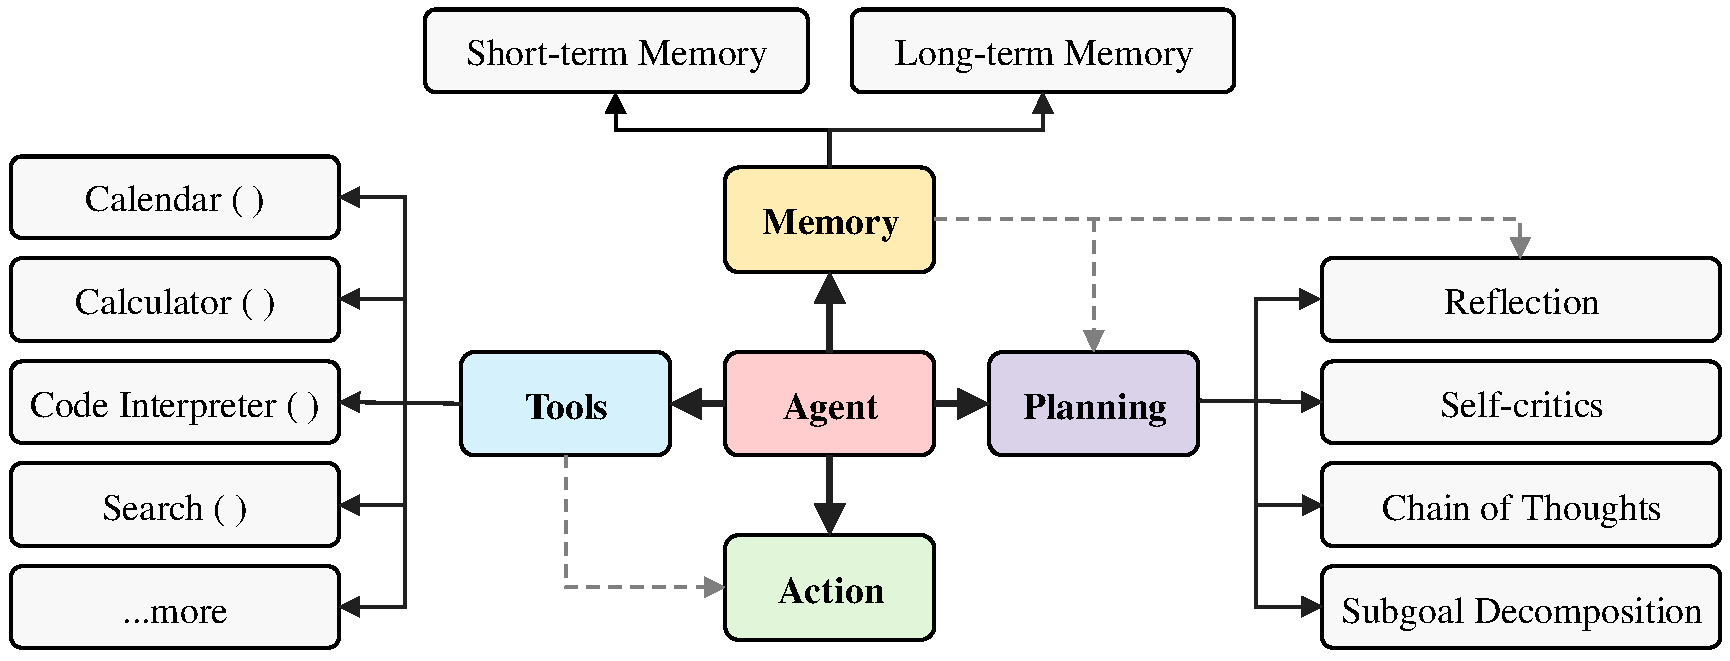
\includegraphics[width=\linewidth]{images/Agent_v4.pdf}
\caption{The general architecture of an LLM-powered autonomous agent system, adapted from \cite{weng2023agent}. \textbf{Planning}: The agent decomposes large tasks into smaller, manageable sub-goals or engages in self-criticism and self-reflection on past actions to learn from mistakes and improve future performance. \textbf{Memory}: This component enables the agent to store and retrieve past information. \textbf{Tools}: The agent is trained to invoke external functions or APIs. \textbf{Action}: The agent executes actions, with or without the use of tools, to interact with the environment. The gray dashed lines represent the data flow within the system.
% The general architecture of an LLM-powered autonomous agent system. The image is borrowed from \cite{weng2023agent}. \textbf{Planning}: The agent breaks down large tasks into smaller, manageable subgoals or does self-criticism and self-reflection over past actions to learn from mistakes and refine them for future steps. \textbf{Memory}: This provides the agent with the capability to retain and recall previous information. \textbf{Tools}: The agent learns to call external functions/APIs. \textbf{Action}: The agent takes action with or without tools to affect the environment. The gray dashed line indicates the data flow.
}
\label{fig:agent}
\end{figure*}

\begin{figure*}[t] \color{blue}
\centering
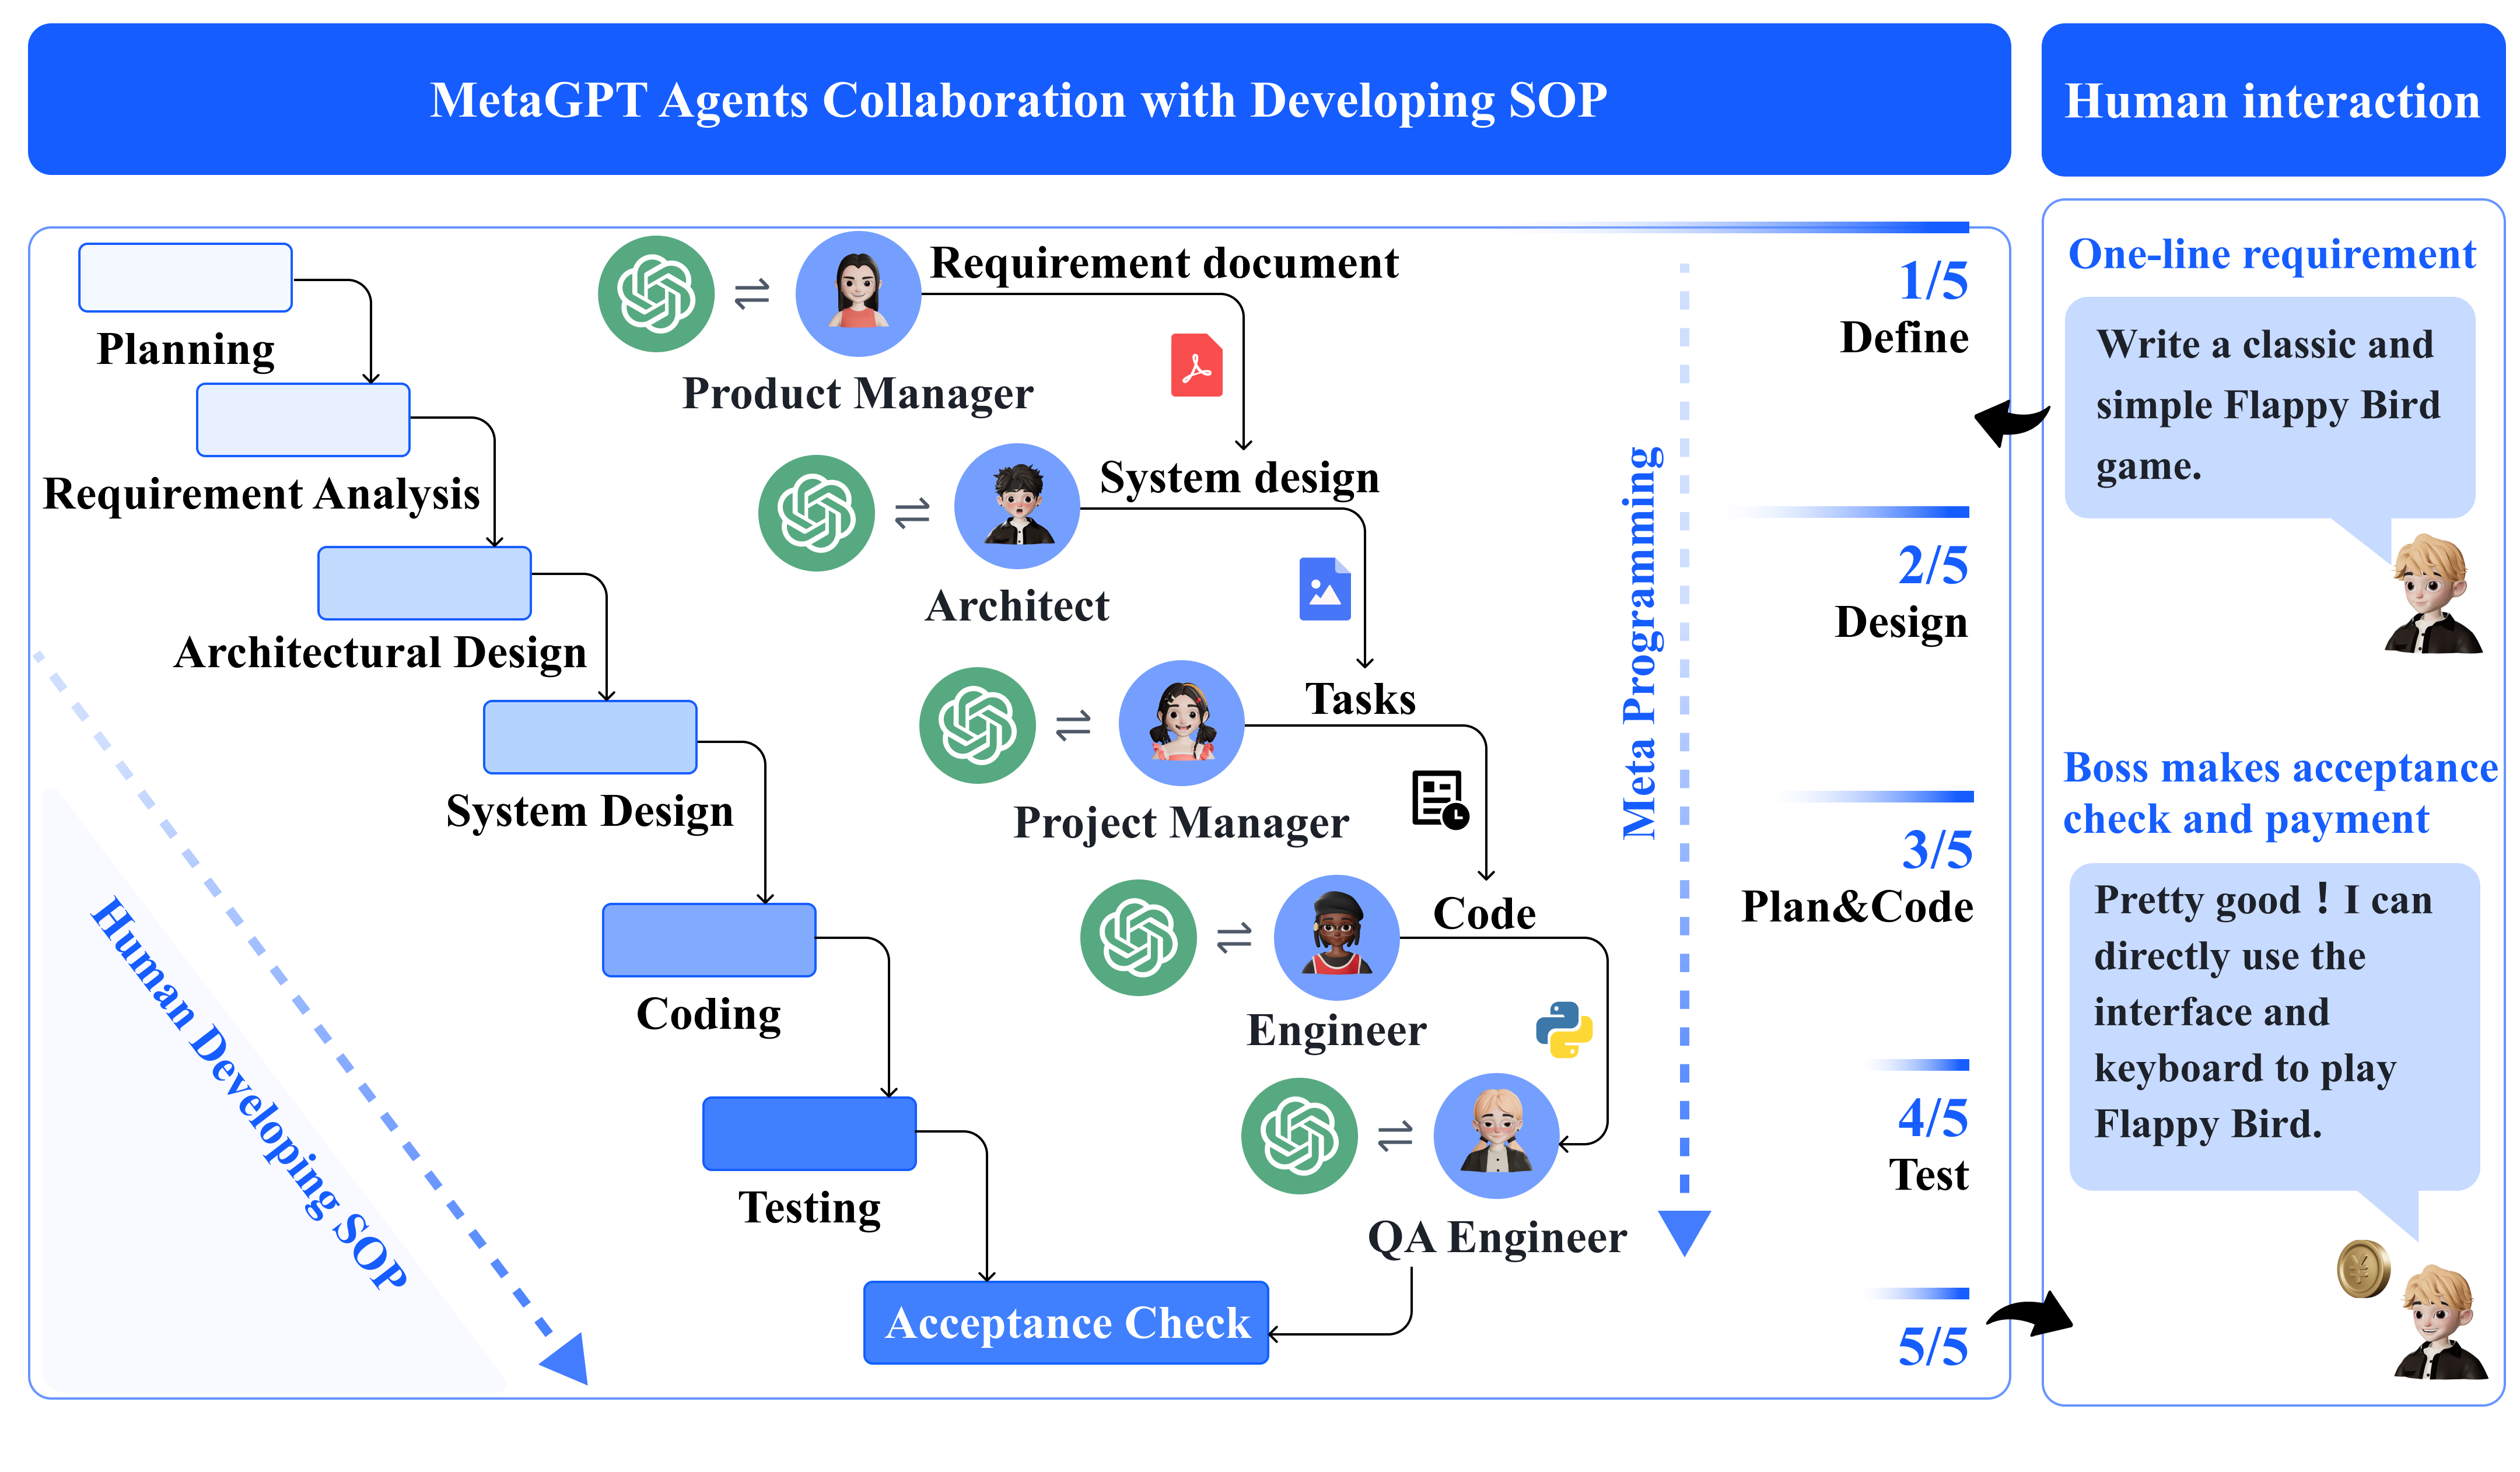
\includegraphics[width=0.95\linewidth]{images/metagpt.png}
\caption{\done{MetaGPT integrates human workflow efficiencies into LLM-based multi-agent collaboration to break down complex code-related tasks into specific, actionable procedures. These procedures are then assigned to various roles, such as Product Manager, Architect, and Engineer played by LLM. The image is sourced from the original paper \cite{hong2023metagpt}.
}}
\label{fig:matagpt}
\end{figure*}


% Recently, an LLM-powered autonomous agent has been adopted to automate code generation and achieve state-of-the-art performance, e.g., AgentCoder \cite{huang2023agentcoder} with 96.3\% Pass@1 on HumanEval, which brings us closer to the future of automated software development \cite{ishibashi2024self}. 
% \cite{hong2023metagpt} proposes an innovative meta-programming framework termed MetaGPT to incorporate efficient human workflows into LLM-based multi-agent collaborations. 
% \cite{huang2023agentcoder} proposes a multi-agent framework termed AgentCoder with three specialized agents with different roles and capabilities, i.e., the programmer agent for code generation, the test designer agent for unit test generation, and the test executor agent for executing code and writing feedback, ensuring more effective code generation. 
% CodeAct \cite{wang2024executable} utilizes executable Python code to consolidate LLM agents’ actions into a unified action space rather than generating JSON or text in a pre-defined format.
% AutoCodeRover \cite{zhang2024autocoderover} is proposed to solve GitHub issues to autonomously achieve program improvement. 
In the realm of automated code generation, LLM-powered autonomous agents have demonstrated remarkable proficiency. 
For instance, AgentCoder \cite{huang2023agentcoder} achieved a groundbreaking \texttt{pass@1} of 96.3\% on the HumanEval benchmark, forwarding a step closer to the future of automated software development \cite{ishibashi2024self}. 
\done{The innovative meta-programming framework termed MetaGPT \cite{hong2023metagpt} integrates human workflow efficiencies into LLM-based multi-agent collaboration, as shown in Figure \ref{fig:matagpt}.}  
Furthermore, \cite{huang2023agentcoder} introduces AgentCoder, a multi-agent framework composed of three specialized agents, each with distinct roles and capabilities. These roles include a programmer agent responsible for code generation, a test designer agent tasked with generating unit test cases, and a test executor agent that executes the code and provides feedback. This division of labor within AgentCoder promotes more efficient and effective code generation.
CodeAct \cite{wang2024executable} distinguishes itself by utilizing executable Python code to consolidate LLM agent actions within a unified action space, in contrast to the generation of JSON or textual formats. 
Additionally, AutoCodeRover \cite{zhang2024autocoderover} is proposed to autonomously resolve GitHub issues for program enhancement.

% To handle more complicated tasks in software engineering, two autonomous AI software engineers Devin\footnote{\href{https://www.cognition.ai/introducing-devin}{https://www.cognition.ai/introducing-devin}}\cite{Devin} and OpenDevin\footnote{\href{https://github.com/OpenDevin/OpenDevin}{https://github.com/OpenDevin/OpenDevin}}\cite{OpenDevin} are released and quickly attracted a lot of attention within a very short time. 
% Subsequently, \cite{swe-agent} presents an autonomous system SWE-agent that uses a language model to interact with a computer to solve software engineering tasks and solve 12.5\% of issues on SWE-bench benchmark \cite{jimenez2023swe}. 
% \cite{holt2023l2mac} presents L2MAC, the first practical LLM-based general-purpose stored-program automatic computer (von Neumann architecture) framework, an LLM-based multi-agent system, for long and consistent output generation.
% During this survey writing, OpenDevin augments CodeAct with tools based on bash commands and releases OpenDevin CodeAct 1.0 \cite{OpenDevin_CodeAct}, achieving a state-of-the-art performance on the SWE-Bench Lite benchmark. 
To address the complexity of tasks within software engineering, two innovative autonomous AI software engineers Devin\footnote{\href{https://www.cognition.ai/introducing-devin}{https://www.cognition.ai/introducing-devin}}\cite{Devin} and OpenDevin\footnote{\href{https://github.com/OpenDevin/OpenDevin}{https://github.com/OpenDevin/OpenDevin}}\cite{OpenDevin}, have been released and rapidly garnered considerable interest within the software engineering (SE) and artificial general intelligence (AGI) community. 
Subsequently, an autonomous system, SWE-agent \cite{swe-agent}, leverages a language model to interact with a computer to address software engineering tasks, successfully resolving 12.5\% of issues on the SWE-bench benchmark \cite{jimenez2023swe}. 
L2MAC \cite{holt2023l2mac} has been introduced as the first practical, LLM-based, multi-agent, general-purpose stored-program automatic computer that utilizes a von Neumann architecture, designed specifically for the generation of long and consistent outputs.
At the time of writing this survey, OpenDevin has enhanced CodeAct with bash command-based tools, leading to the release of OpenDevin CodeAct 1.0 \cite{OpenDevin_CodeAct}, which sets a new state-of-the-art performance on the SWE-Bench Lite benchmark \cite{jimenez2023swe}.

% Despite such exciting progress, AI software engineers with LLM-powered autonomous agents still have a long way to go \cite{xi2023rise,wang2024survey}. In particular, the design of prompts, the context length, the number of agents, and the set of tools are worthy of further thinking and optimization, as the problem complexity increases \cite{ishibashi2024self}.
Despite these remarkable advancements, the journey toward fully realized AI software engineers employing LLM-powered autonomous agents is far from complete \cite{xi2023rise,wang2024survey}. Critical aspects such as prompt design, context length, agent count, and toolsets call for further refinement and optimization, especially as problem complexities escalate \cite{ishibashi2024self}.

%%%%%%%%%%%%%%%%%%%%%%%%%%%%%%%%%%%%%%%%%%%%%%%%%%%%%%%%%%%%%%%%%%%%%%%%
%%%%%%%%%%%%%%%%%%%%%%%%%%%%%%%%%%%%%%%%%%%%%%%%%%%%%%%%%%%%%%%%%%%%%%%%
\subsection{Evaluation}\label{sec:evaluation}
\begin{table}[t!] 
% \begin{wraptable}{R}{0.5\linewidth}
\caption{
% The Performance (\texttt{Pass@1}, \texttt{Pass@10}, and \texttt{Pass@100}) comparison of LLMs for code generation on HumanEval benchmark. For the model with various model size, we only report the largest size version of each model.
\done{The performance comparison of LLMs for code generation on the HumanEval \cite{chen2021evaluating} benchmark, measured by \texttt{Pass@1}. 
% Due to the limitations of computational resources we faced, we directly cite the experimental results from the original papers or widely recognized open-source leaderboard in research community.
For models with various sizes, we report only the largest size version of each model with a magnitude of \texttt{B} parameters. $^\ddag$ denotes instruction-tuned models.
% DeepSeek-Coder-V2-Instruct is an open-source Mixture-of-Experts (MoE) code language
% model, which has 236B parameters with only 21B activation parameters. 
} 
}
\label{tab:performance_humaneval}
\centering
\scalebox{0.75}{
\rotatebox{0}{
    \begin{tabular}{clrcc}
    \toprule
    & \textbf{Model} & \textbf{Size} & \texttt{pass@1} (\%) & \textbf{Availability} \\ 
       % &   &   & $k=1$ & $k=10$ & $k=100$ & \\ 
\midrule
    \multirow{17}{*}{\textbf{Closed Source}} 
         & GPT-4o-0513 \cite{gpt-4o} & - & 91.0 & \href{https://openai.com/index/hello-gpt-4o/}{[API Access]} \\
         & GPT-4-Turbo-0409 \cite{gpt-4-turbo} & - & 88.2 &  \href{https://openai.com/blog/new-models-and-developer-products-announced-at-devday}{[API Access]} \\
         & GPT-4-1106 \cite{achiam2023gpt}& - & 87.8  & \href{https://openai.com/index/gpt-4/}{[API Access]} \\
         & GPT-3.5-Turbo-0125 \cite{gpt-3.5-turbo}& - & 76.2  & \href{https://openai.com/index/new-embedding-models-and-api-updates}{[API Access]} \\
         & \cellcolor{yellow!40}Claude-3.5-Sonnet \cite{claude3} & \cellcolor{yellow!40}- & \cellcolor{yellow!40}\textbf{92.0} & \href{https://claude.ai/}{[API Access]} \\
         & Claude-3-Opus \cite{claude3} & - & 84.9 & \href{https://www.anthropic.com/news/claude-3-family}{[API Access]} \\
         & Claude-3-Sonnet \cite{claude3} & - & 73.0 & \href{https://www.anthropic.com/news/claude-3-family}{[API Access]} \\
         & Claude-3-Haiku \cite{claude3} & - & 75.9 & \href{https://www.anthropic.com/news/claude-3-family}{[API Access]} \\
         & Gemini-1.5-Pro \cite{reid2024gemini} & - & 84.1 & \href{https://deepmind.google/technologies/gemini/pro/}{[API Access]} \\
         & Gemini-1.5-Flash \cite{reid2024gemini} & - & 74.3 & \href{https://deepmind.google/technologies/gemini/flash/}{[API Access]} \\
         & Gemini-1.0-Ultra \cite{reid2024gemini} & - & 74.4 & \href{https://deepmind.google/technologies/gemini/ultra/}{[API Access]} \\
         & Gemini-1.0-Pro \cite{reid2024gemini} & - & 67.7 & \href{https://deepmind.google/technologies/gemini/pro/}{[API Access]} \\
         \cline{2-5}
         & $^\ddag$PanGu-Coder2 \cite{shen2023pangu} & 15B & 61.64     & - \\
         & PanGu-Coder \cite{christopoulou2022pangu} & 2.6B & 23.78        & - \\
         & Codex \cite{chen2021evaluating} & 12B & 28.81 & Deprecated \\
         & PaLM-Coder \cite{chowdhery2023palm} & 540B & 36     & - \\
         & AlphaCode \cite{li2022competition} & 1.1B & 17.1     & - \\
         \midrule
    \multirow{36}{*}{\textbf{Open Source}} 
         & $^\ddag$Codestral \cite{codestral} & 22B & 81.1 &  \href{https://huggingface.co/mistralai/Codestral-22B-v0.1}{[Checkpoint Download]} \\
         & \cellcolor{yellow!40}$^\ddag$DeepSeek-Coder-V2-Instruct \cite{zhu2024deepseek}  & \cellcolor{yellow!40}21B (236B) & \cellcolor{yellow!40}\textbf{90.2} & \href{https://huggingface.co/deepseek-ai/DeepSeek-Coder-V2-Instruct}{[Checkpoint Download]}\\
         & \cellcolor{yellow!40}$^\ddag$Qwen2.5-Coder-Instruct \cite{hui2024qwen2} & \cellcolor{yellow!40}7B & \cellcolor{yellow!40}88.4 & \href{https://huggingface.co/Qwen/Qwen2.5-Coder-7B-Instruct}{[Checkpoint Download]}\\
         & Qwen2.5-Coder \cite{hui2024qwen2} & 7B & 61.6  & \href{https://huggingface.co/Qwen/Qwen2.5-Coder-7B}{[Checkpoint Download]}\\
         & $^\ddag$StarCoder2-Instruct \cite{starcoder2instruct} &  15.5B  & 72.6 & \href{https://huggingface.co/bigcode/starcoder2-15b-instruct-v0.1}{[Checkpoint Download]} \\
         % Llama3 \cite{llama3} & 70B & 81.7 & - & - & \href{}{[Checkpoint Download]}  \\
         & $^\ddag$CodeGemma-Instruct \cite{codegemma_2024}  & 7B  & 56.1  & \href{https://huggingface.co/google/codegemma-7b-it}{[Checkpoint Download]}  \\
         & CodeGemma \cite{codegemma_2024}  & 7B  & 44.5  & \href{https://huggingface.co/google/codegemma-7b}{[Checkpoint Download]}  \\
         & StarCoder 2 \cite{lozhkov2024starcoder}  & 15B & 46.3 & \href{https://huggingface.co/bigcode/starcoder2-15b}{[Checkpoint Download]}\\
         % phi-2 \cite{phi-2}   & 2.7B & 49.4 & - & - & \href{}{[Checkpoint Download]}  \\
         & $^\ddag$WaveCoder-Ultra \cite{yu2023wavecoder} & 6.7B & 79.9  & \href{https://huggingface.co/microsoft/wavecoder-ultra-6.7b}{[Checkpoint Download]}  \\
         & $^\ddag$WaveCoder-Pro \cite{yu2023wavecoder} & 6.7B & 74.4  & \href{https://huggingface.co/microsoft/wavecoder-pro-6.7b}{[Checkpoint Download]}  \\
         & $^\ddag$WaveCoder-DS \cite{yu2023wavecoder} & 6.7B & 65.8  & \href{https://huggingface.co/microsoft/wavecoder-ds-6.7b}{[Checkpoint Download]}  \\
         & StableCode \cite{pinnaparaju2024stable} & 3B & 29.3  & \href{https://huggingface.co/stabilityai/stable-code-3b}{[Checkpoint Download]}  \\
         & CodeShell \cite{xie2024codeshell} & 7B & 34.32  & \href{https://huggingface.co/WisdomShell/CodeShell-7B}{[Checkpoint Download]}  \\
         & $\ddag$CodeQwen1.5-Chat \cite{codeqwen} & 7B & 83.5 & \href{https://huggingface.co/Qwen/CodeQwen1.5-7B-Chat}{[Checkpoint Download]}  \\
         & CodeQwen1.5 \cite{codeqwen} & 7B & 51.8 & \href{https://huggingface.co/Qwen/CodeQwen1.5-7B}{[Checkpoint Download]}  \\
         & $^\ddag$DeepSeek-Coder-Instruct \cite{guo2024deepseek} & 33B & 79.3  & \href{https://huggingface.co/deepseek-ai/deepseek-coder-33b-instruct}{[Checkpoint Download]}  \\
         & DeepSeek-Coder \cite{guo2024deepseek} & 33B & 56.1  & \href{https://huggingface.co/deepseek-ai/deepseek-coder-33b-base}{[Checkpoint Download]}  \\
         & replit-code \cite{replit-code} & 3B & 20.12  & \href{https://huggingface.co/replit/replit-code-v1-3b}{[Checkpoint Download]}  \\
         % Phi-1.5 \cite{li2023textbooks} & 1.3B & 41.4 & - & - & \href{}{[Checkpoint Download]}  \\
         & $^\ddag$Magicoder$S$-CL \cite{wei2023magicoder} & 7B & 70.7 & \href{https://huggingface.co/ise-uiuc/Magicoder-S-CL-7B}{[Checkpoint Download]} \\
         & $^\ddag$Magicoder-CL \cite{wei2023magicoder} & 7B & 60.4 & \href{https://huggingface.co/ise-uiuc/Magicoder-CL-7B}{[Checkpoint Download]}\\
         & $^\ddag$WizardCoder \cite{luo2023wizardcoder} & 33B & 79.9        & \href{https://huggingface.co/WizardLM/WizardCoder-33B-V1.1}{[Checkpoint Download]}  \\
         & CodeFuse \cite{liu2023mftcoder} & 34B & 74.4     & \href{https://huggingface.co/TheBloke/CodeFuse-CodeLlama-34B-GGUF}{[Checkpoint Download]}  \\
         & Phi-1 \cite{gunasekar2023textbooks} & 1.3B & 50.6          & \href{https://huggingface.co/microsoft/phi-1}{[Checkpoint Download]}  \\
         & $^\ddag$Code Llama-Instruct \cite{roziere2023code} & 70B & 67.8 & \href{https://huggingface.co/codellama/CodeLlama-70b-Instruct-hf}{[Checkpoint Download]}  \\
         & Code Llama \cite{roziere2023code} & 70B & 53.0  & \href{https://huggingface.co/codellama/CodeLlama-70b-hf}{[Checkpoint Download]}  \\
         & $^\ddag$OctoCoder \cite{muennighoff2023octopack} & 15.5B & 46.2   & \href{https://huggingface.co/bigcode/octocoder}{[Checkpoint Download]}  \\
         & CodeGeeX2 \cite{zheng2023codegeex} & 6B & 35.9          & \href{https://huggingface.co/THUDM/codegeex2-6b}{[Checkpoint Download]}  \\
         & $^\ddag$InstructCodeT5+ \cite{wang2023codet5+} & 16B & 35.0          & \href{https://huggingface.co/Salesforce/instructcodet5p-16b}{[Checkpoint Download]}  \\
         % CodeGen \cite{nijkamp2022codegen} & 16.1B & 34.6    & -        & -         & \href{}{[Checkpoint Download]}  \\
        & CodeGen-NL \cite{nijkamp2022codegen} & 16.1B & 14.24             & \href{https://huggingface.co/Salesforce/codegen-16B-nl}{[Checkpoint Download]}  \\
        & CodeGen-Multi \cite{nijkamp2022codegen} & 16.1B & 18.32        & \href{https://huggingface.co/Salesforce/codegen-16B-multi}{[Checkpoint Download]}  \\
        & CodeGen-Mono \cite{nijkamp2022codegen} & 16.1B & 29.28           & \href{https://huggingface.co/Salesforce/codegen-16B-mono}{[Checkpoint Download]}  \\
        & StarCoder \cite{li2023starcoder} & 15B & 33.60     & \href{https://huggingface.co/bigcode/starcoder}{[Checkpoint Download]}  \\
        & CodeT5+ \cite{wang2021codet5} & 16B & 30.9    & \href{https://huggingface.co/Salesforce/codet5p-16b}{[Checkpoint Download]}  \\
        % LLaMA2 \cite{touvron2023llama2} & 70B & 30.5    & 59.4     & 87.0      & \href{}{[Checkpoint Download]}  \\
        % PaLM \cite{chowdhery2023palm} & 540B & 26.2    & -        & 76.2      & \href{}{[Checkpoint Download]}  \\
        % LLaMA \cite{touvron2023llama} & 65B & 23.7    & -        & 79.3      & \href{}{[Checkpoint Download]}  \\
        % & CodeGeeX \cite{zheng2023codegeex} & 13B & 22.89       &   \\
        & CodeGen2 \cite{nijkamp2023codegen2} & 16B & 20.46       & \href{https://huggingface.co/Salesforce/codegen2-16B_P}{[Checkpoint Download]}  \\
         & SantaCoder \cite{allal2023santacoder} & 1.1B & 14.0        & \href{https://huggingface.co/bigcode/santacoder}{[Checkpoint Download]}  \\
         % BLOOM \cite{le2023bloom} & 176B & 15.52     & 32.20   & 55.45& \href{}{[Checkpoint Download]}  \\
         % GPT-NeoX \cite{black2022gpt} & 20B & 15.4      & 25.6    & 41.2& \href{}{[Checkpoint Download]}  \\
         & InCoder \cite{fried2022incoder} & 6.7B & 15.2     & \href{https://huggingface.co/facebook/incoder-6B}{[Checkpoint Download]}  \\
         % LaMDA & 137B & 14.0      & -       & 47.3& \href{}{[Checkpoint Download]}  \\
         % GPT-J \cite{gpt-j} & 6B & 11.62     & 15.74   & 27.74& \href{}{[Checkpoint Download]}  \\
         % PyCodeGPT \cite{zan2022cert} & 110M & 8.33      & 13.36   & 19.13& \href{}{[Checkpoint Download]}  \\
         % GPT-Neo \cite{gpt-neo} & 2.7B & 6.41      & 11.27   & 21.37& \href{}{[Checkpoint Download]}  \\
         & PolyCoder \cite{xu2022systematic} & 2.7B & 5.59   & \href{https://huggingface.co/NinedayWang/PolyCoder-2.7B}{[Checkpoint Download]}  \\
         % JuPyT5 \cite{chandel2022training} & 300M & 5.4       & 15.46   & 25.60& \href{}{[Checkpoint Download]}  \\
         & CodeParrot \cite{tunstall2022natural} & 1.5B & 3.99   & \href{https://huggingface.co/codeparrot/codeparrot}{[Checkpoint Download]} \\  
    \bottomrule
    \end{tabular}
}
}
\vspace{-10pt}
% \end{wraptable}
\end{table}
% Despite the powerfulness of large language models, they have showcased many unprecedented behaviors, some of which increase the performance across a wide range of downstream tasks while also bringing potential risk, leading to an unreliable and trustworthy LLM \cite{chen2021evaluating,xu2022systematic,chang2024survey}. 
% Therefore, it is non-trivial to accurately evaluate how they behave to distinguish between good and bad models, encouraging further enhancements in the abilities of LLMs. 
Despite the impressive capabilities of \done{LLMs}, they exhibit a range of behaviors that are both beneficial and potentially risky. 
These behaviors can enhance performance across various downstream tasks but may also introduce reliability and trustworthiness concerns in LLM deployment \cite{chen2021evaluating, xu2022systematic, chang2024survey}. 
Consequently, it is imperative to develop precise evaluation approaches to discern the qualitative and quantitive differences between models, thereby encouraging further advancements in LLM capabilities.

% Similar to general-purpose LLMs, the approaches of evaluating LLMs for code generation can be divided into three categories, namely metrics-based approach, human-based approach, and LLM-based approach. The existing benchmarks for evaluation can be found in Section \ref{sec:benchmark}.
% In the following subsection, we will delve into each category. 
% In the realm of code generation, the evaluation approaches for LLMs can be broadly categorized into three distinct approaches: metrics-based, human-centered, and LLM-informed. Comprehensive benchmarks for evaluation are detailed in Section \ref{sec:benchmark}. 
% In the following subsection, we will provide an in-depth examination of each category of evaluation.
Evaluation strategies for LLMs in code generation mirror those for general-purpose LLMs and can be divided into three principal categories: metrics-based, human-centered, and LLM-based approaches. 
Detailed benchmarks for these evaluation strategies are presented in Section \ref{sec:benchmark} and summarized in Table \ref{tab:benchmark}. 
Subsequent subsections will provide a thorough analysis of each approach.

\subsubsection{Metrics}
% The quest for reliable and robust automatic evaluation metrics for generated content has been a long-standing question in natural language processing \cite{chen1998evaluation,papineni2002bleu,lin2004rouge}.
% At the early stage, most works directly adopt token-matching-based metrics commonly used in text generation, such as Exact Match, BLEU \cite{papineni2002bleu}, ROUGE \cite{lin2004rouge}, and METEOR \cite{banerjee2005meteor}, to evaluate the quality of generated code.
The pursuit of effective and reliable automatic evaluation metrics for generated content is a long-standing challenge within the field of natural language processing (NLP) \cite{chen1998evaluation, papineni2002bleu, lin2004rouge}. 
At the early stage, most works directly leverage token-matching-based metrics, such as Exact Match, BLEU \cite{papineni2002bleu}, ROUGE \cite{lin2004rouge}, and METEOR \cite{banerjee2005meteor}, which are prevalent in text generation of NLP, to assess the quality of code generation.

% While these metrics provide a quick and cost-effective means of evaluating the quality of the generated code, they often fall short of precisely evaluating the syntactical and functional correctness and semantic features of generated code.
% To eliminate this issue, CodeBLEU \cite{ren2020codebleu} is proposed to absorb the strength of BLEU in the n-gram match and further inject code syntax via abstract syntax trees (AST) and code semantics via data-flow. 
% Nevertheless, the generated code still suffers from error running and has a different execution result. 
% Thus, the more prevalent evaluation methods for code generation are execution-based metrics, including \texttt{pass@k} \cite{chen2021evaluating}, \texttt{n@k} \cite{li2022competition}, test case average \cite{hendrycks2021measuring}, execution accuracy \cite{rajkumar2022evaluating}, and \texttt{pass@t} \cite{olausson2023self}.
% Among them, \texttt{pass@k} as the primary evaluation metric estimates the rate for which $\geq$1 of $k$ model samples passes all the unit tests. An unbiased estimator introduced by \cite{chen2021evaluating} can be formulated as 
While these metrics offer a rapid and cost-effective approach for assessing the quality of generated code, they often fall short of capturing the syntactical and functional correctness, as well as the semantic features of the code. 
To eliminate this limitation, CodeBLEU \cite{ren2020codebleu} was introduced, enhancing the traditional BLEU metric \cite{papineni2002bleu} by incorporating syntactic information through abstract syntax trees (AST) and semantic understanding via data-flow graph (DFG). 
Despite these improvements, the metric does not fully resolve issues pertaining to execution errors or discrepancies in the execution results of the generated code.
In light of these challenges, execution-based metrics have gained prominence for evaluating code generation, including \texttt{pass@k} \cite{chen2021evaluating}, \texttt{n@k} \cite{li2022competition}, test case average \cite{hendrycks2021measuring}, execution accuracy \cite{rajkumar2022evaluating}, and \texttt{pass@t} \cite{olausson2023self}. 
In particular, the \texttt{pass@k}, serving as a principal evaluation metric, assesses the probability that at least one out of $k$ code samples generated by a model will pass all unit tests. An unbiased estimator for \texttt{pass@k} introduced by \cite{chen2021evaluating} is defined as: 
\begin{equation}\label{eq:pass@k}
\begin{aligned}
    \texttt{pass@k} \coloneqq \mathbb{E}_\text{task} \left[1-\frac{\binom{n-c}{k}}{\binom{n}{k}}\right]
\end{aligned} 
\end{equation}
% where $n$ and $k$ are the numbers of sampling candidate code solutions and randomly sampled code solutions from the sampling candidates for each programming problem respectively, and $n\ge k$, $c$ is the number of correct ones in $k$ samples.
% Table \ref{tab:performance_humaneval} and \ref{tab:performance_mbpp} showcase the performance of existing LLMs for code generation on \texttt{pass@k} metrics with $k\in\{1, 10, 100\}$ over HumanEval and MBPP benchmarks, respectively.
where $n$ is the total number of sampled candidate code solutions, $k$ is the number of randomly selected code solutions from these candidates for each programming problem, with $n\ge k$, and $c$ is the count of correct samples within the $k$ selected. 

% However, these approaches have stringent requirements for the quality of unit tests and can only evaluate executable code \cite{zan2023large}. 
% Therefore, non-executable evaluation methods (i.e., token-matching-based metrics) become an alternative method when unit tests are not available. 
% Furthermore, in the absence of a ground truth label, an unsupervised metrics perplexity (PPL) \cite{jelinek1977perplexity} can be used for evaluation, which measures how well an LLM generalizes to unseen data by calculating the model's uncertainty in predicting new content. It provides a potential reference value for the quality of the generated code.
Nevertheless, these execution-based methods are heavily dependent on the quality of unit tests and are limited to evaluating executable code \cite{zan2023large}. Consequently, when unit tests are unavailable, token-matching-based metrics are often employed as an alternative for evaluation. 
Furthermore, in scenarios lacking a ground truth label, unsupervised metrics such as perplexity (PPL) \cite{jelinek1977perplexity} can serve as evaluative tools. Perplexity quantifies an LLM's uncertainty in predicting new content, thus providing an indirect measure of the model's generalization capabilities and the quality of the generated code.

% Taken together, no matter which above methods are used, they only consider the functional correctness of the code, lacking a comprehensive evaluation of the various aspects of code, such as vulnerability \cite{nappa2015attack}, maintainability \cite{ardito2020tool}, readability \cite{buse2009learning}, complexity and efficiency \cite{peitek2021program}, style consistency \cite{markovtsev2019style} and running stability \cite{raemaekers2012measuring}.
Taken together, while the aforementioned methods primarily focus on the functional correctness of code, they do not provide a holistic evaluation that encompasses other critical dimensions such as code vulnerability \cite{nappa2015attack}, maintainability \cite{ardito2020tool}, readability \cite{buse2009learning}, complexity and efficiency \cite{peitek2021program}, stylistic consistency \cite{markovtsev2019style}, and execution stability \cite{raemaekers2012measuring}. 
A comprehensive evaluation framework that integrates these aspects remains an open area for future research and development in the field of code generation assessment.

\subsubsection{Human Evaluation}
% Due to the inherent properties of code, above mentioned automatic evaluation metrics can only solve partial aspects of code evaluation. 
% For example, code style consistency is difficult to design specific metrics to measure in most cases \cite{chen2023duetcs}. 
% For repository-level code generation, it is significantly difficult to measure overall code quality with a simple metric due to the characteristic of larger scale, cross-file design, and complex internal and external dependencies \cite{bairi2023codeplan,shrivastava2023repofusion}.
Given the intrinsic characteristics of code, the aforementioned automatic evaluation metrics are inherently limited in their capacity to fully assess code quality. 
For instance, metrics specifically designed to measure code style consistency are challenging to develop and often fail to capture this aspect adequately \cite{chen2023duetcs}. 
When it comes to repository-level code generation, the evaluation of overall code quality is substantially complicated due to the larger scale of the task, which involves cross-file designs and intricate internal as well as external dependencies, as discussed by \cite{bairi2023codeplan,shrivastava2023repofusion}.

% To eliminate these challenges, it necessitates conducting human evaluation, yielding relatively solid and reliable results. 
% Besides, human evaluation provides more flexibility in diverse evaluation tasks, simplifying complex and multi-step evaluation. 
% Furthermore, human evaluation also plays a vital role in showing the efficacy of some token-matching-based metrics, e.g., CodeBLEU \cite{ren2020codebleu}. 
% These works often conduct experiments by evaluating the correlation coefficient between proposed metrics and quality scores assigned by the real users to show superior performance compared with existing metrics.  
To overcome these challenges, conducting human evaluations becomes necessary, as it yields relatively robust and reliable results.
Human assessments also offer greater adaptability across various tasks, enabling the simplification of complex and multi-step evaluations. 
Moreover, human evaluations are essential for demonstrating the effectiveness of certain token-matching-based metrics, such as CodeBLEU \cite{ren2020codebleu}. 
These studies typically conduct experiments to evaluate the correlation coefficient between proposed metrics and quality scores assigned by actual users, demonstrating their superiority over existing metrics.

% Moreover, to align the large language models with human preferences or intent, InstructGPT \cite{ouyang2022training} utilizes labeler-written prompts and demonstrations and ranking of model outputs to fine-tune LLMs using reinforcement learning from human feedback (RLHF). 
% Recently, alignment learning with feedback has been adopted for code generation tasks. But due to the nature of code, the feedback is generally conducted by a compiler or interpreter rather than a human being to provide execution feedback, such as CodeRL \cite{le2022coderl}, PPOCoder \cite{shojaee2023execution}, RLTF \cite{liu2023rltf}, and PanGu-Coder2 \cite{shen2023pangu}. More details can be found in Section \ref{sec:reinforcement_learning}.
Moreover, in an effort to better align \done{LLMs} with human preferences and intentions, InstructGPT \cite{ouyang2022training} employs human-written prompts and demonstrations, and model output ranking in the fine-tuning of LLMs using reinforcement learning from human feedback (RLHF). 
Although similar alignment learning techniques have been applied to code generation, the feedback in this domain typically comes from a compiler or interpreter, which offers execution feedback, rather than from human evaluators. 
Notable examples include CodeRL \cite{le2022coderl}, PPOCoder \cite{shojaee2023execution}, RLTF \cite{liu2023rltf}, and PanGu-Coder2 \cite{shen2023pangu}. 
Further information on this topic is available in Section \ref{sec:reinforcement_learning}.

% Despite these pros, human evaluation also has inherent cons that could potentially affect its accuracy and consistency. For example, 
% 1) personalized tastes and varying education levels among human evaluators can introduce biases or even inconsistencies in the evaluation process; 
% 2) conducting robust and reliable human evaluations often requires a large number of evaluators, which can be very expensive and time-consuming;
% 3) human evaluation is often not reproducible, making it infeasible to extend existing evaluation results or track the progress of LLMs \cite{zhao2023survey}.
Nonetheless, human evaluations are not without drawbacks, as they can be prone to certain issues that may compromise their accuracy and consistency. 
For instance, 
1) personalized tastes and varying levels of expertise among human evaluators can introduce biases and inconsistencies into the evaluation process;
2) conducting comprehensive and reliable human evaluations often necessitates a substantial number of evaluators, leading to significant expenses and time-consuming;
3) the reproducibility of human evaluations is often limited, which presents challenges in extending previous evaluation outcomes or monitoring the progress of LLMs, as highlighted by \cite{zhao2023survey}.

\subsubsection{LLM-as-a-Judge}
\begin{figure*}[t]
\centering
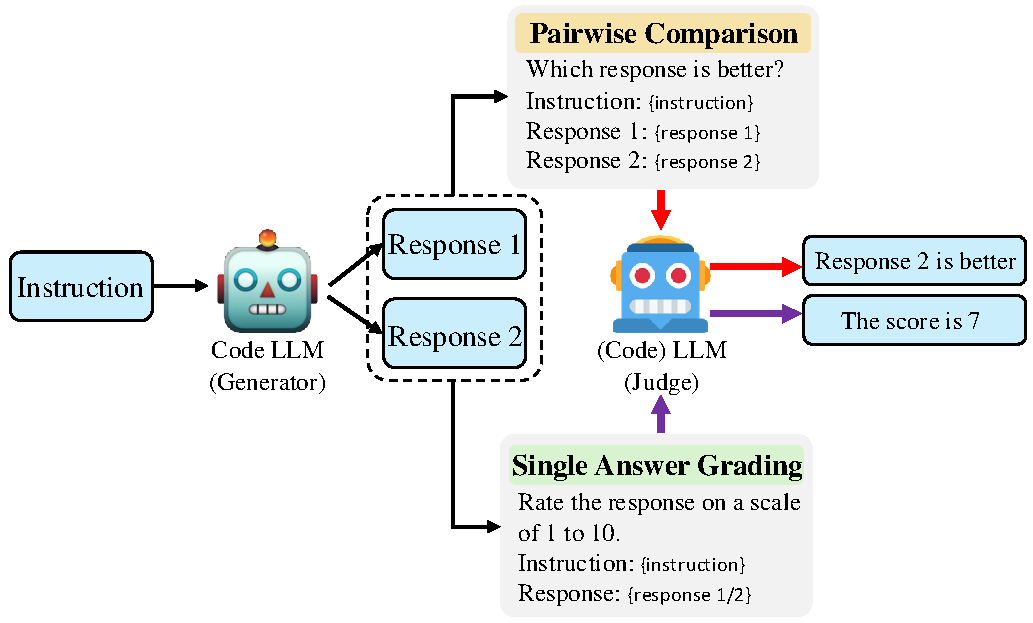
\includegraphics[width=0.95\linewidth]{images/llm-as-judge_v4.pdf}
\caption{\done{The pipeline of (Code) LLM-as-a-judge for evaluating generated code by Code LLMs. There are primarily two types of approaches: pairwise comparison and single answer grading.} 
}
\label{fig:llm-as-judge}
\end{figure*}
% The powerful instruction-following capabilities of LLM inspire researchers to innovatively explore the possibility of LLM-based evaluation. 
% LLM-as-a-Judge \cite{zheng2024judging} refers to use strong closed-source LLMs (e.g., GPT4, Gemini, and Claud 3) as the surrogate of human evaluators and design prompts with some requirements to guide LLMs to conduct evaluation, such as AlpacaEval \cite{alpaca_eval} and MT-bench \cite{zheng2024judging}. 
% It diminishes the reliance on human involvement and enables more efficient and scalable evaluation. 
% In addition, LLMs can provide meaningful explanations for the assigned rating scores, thereby enhancing the interpretability of evaluations \cite{zhao2023survey}. 
The powerful instruction-following capabilities of \done{LLMs} have stimulated researchers to innovatively investigate the potential of LLM-based evaluations. 
The LLM-as-a-Judge \cite{zheng2024judging} refers to the application of advanced proprietary LLMs (e.g., GPT4, Gemini, and Claud 3) as proxies for human evaluators. This involves designing prompts with specific requirements to guide LLMs in conducting evaluations, as demonstrated by AlpacaEval \cite{alpaca_eval} and MT-bench \cite{zheng2024judging}. 
This method reduces reliance on human participation, thereby facilitating more efficient and scalable evaluations. 
Moreover, LLMs can offer insightful explanations for the assigned rating scores, thereby augmenting the interpretability of evaluations \cite{zhao2023survey}.

% However, employing LLM-based evaluation for code generation is yet scarce compared with the general-purpose LLM. 
% One of the recently released works \cite{zhuo2024ice} proposes ICE-Score evaluation metric via instructing LLM for code assessments, achieving superior correlations with functional correctness and human preferences, without the need for test oracles or references. 
% With the further enhancement of LLM capabilities, we expect to see more of this line of work in the future.
Nevertheless, the use of LLM-based evaluation for code generation remains relatively underexplored compared with general-purpose LLM. 
\done{The pipeline of (Code) LLM-as-a-judge for evaluating generated code by Code LLMs is depicted in Figure \ref{fig:llm-as-judge}.}
A recent work \cite{zhuo2024ice} introduces the ICE-Score evaluation metric, which instructs LLM for code assessments. 
% This approach achieves superior correlations with functional correctness and human preferences, eliminating the need for test oracles or references. 
This approach attains superior correlations with functional correctness and human preferences, thereby eliminating the requirement for test oracles or references.
As the capabilities of LLM continue to improve, we anticipate seeing more research in this direction.

% Despite their scalability and explainability, LLM-based evaluation is limited by the upper bound of selected LLM capabilities. 
% It has been found that most LLMs including GPT4 suffer from several issues, including position, verbosity, and self-enhancement bias, as well as limited reasoning ability \cite{zheng2024judging}.
Despite their scalability and explainability, the effectiveness of LLM-based evaluation is constrained by the inherent limitations of the chosen LLM. 
Several studies have shown that most LLMs, including GPT-4, suffer from several issues, including position, verbosity, and self-enhancement biases, as well as restricted reasoning ability \cite{zheng2024judging}.
% Specifically, position bias (i.e., the order to present the responses) refers to the fact that LLMs tend to assign high scores for the answers at specific positions over others, 
% verbosity bias means that LLMs favor verbose answers even if they are short in quality compared with shorter answers, and 
% self-enhancement bias indicates that LLMs often overrate in their own generations \cite{zheng2024judging,zhao2023survey}. 
% In addition, since LLMs have limited capacities in solving complex reasoning problems, they cannot serve as qualified evaluators for some reasoning-intensive tasks (e.g., mathematical reasoning).
% These limitations can be mitigated to some extent by specific prompt engineering and fine-tuning strategies \cite{zheng2024judging}. 
Specifically, position bias refers to the tendency of \done{LLMs} to disproportionately favor responses that are presented in certain positions, which can skew the perceived quality of answers based on their order of presentation. 
Meanwhile, verbosity bias describes the inclination of LLMs to prefer lengthier responses, even when these are not necessarily of higher quality compared to more concise ones. 
Self-enhancement bias, on the other hand, is observed when LLMs consistently overvalue the quality of the text they generate \cite{zheng2024judging,zhao2023survey}.
Moreover, due to their inherent limitations in tackling complex reasoning challenges, LLMs may not be entirely reliable as evaluators for tasks that require intensive reasoning, such as those involving mathematical problem-solving.
However, these shortcomings can be partially addressed through the application of deliberate prompt engineering and fine-tuning techniques, as suggested by \cite{zheng2024judging}.


\done{\subsubsection{Empirical Comparison}
% \begin{table}[t]
% % \begin{wraptable}{R}{0.5\linewidth}
% \caption{The performance comparison of LLMs for code generation on the MBPP \cite{austin2021program} benchmark, measured by \texttt{Pass@1}. For models with various sizes, we report only the largest size version of each model with the magnitude of \texttt{B} parameters.}
% \label{tab:performance_mbpp}
% \centering
% \scalebox{0.75}{
% \rotatebox{0}{
%     \begin{tabular}{lrc}
%     \toprule
%     \textbf{Model} & \textbf{Size} & \texttt{pass@1} \\ 
% \midrule
%     % GPT-4  & - &    \\ 
%     GPT-3.5-Turbo \cite{gpt-3.5-turbo} & - & 52.2   \\
%     Claude-3-Opus \cite{claude3} & - & 86.4 \\
%     Claude-3-Sonnet \cite{claude3} & - & 79.4 \\
%     Claude-3-Haiku \cite{claude3} & - & 80.4 \\
%     \midrule
%     Codestral & 22B & 78.2 \\
%     Qwen2.5-Coder-Instruct & 7B & 83.5 \\
%     Qwen2.5-Coder & 7B & 76.9 \\
%     StarCoder2-Instruct \cite{starcoder2instruct} &  15.5B  & 75.2 \\
%     CodeGemma-Instruct \cite{codegemma_2024}  & 7B  & 54.2 \\
%     CodeGemma \cite{codegemma_2024}  & 7B  & 56.2 \\
%     StarCoder 2 \cite{lozhkov2024starcoder}  & 15B & 66.2 \\
%     WaveCoder \cite{yu2023wavecoder} & 6.7B & 74.9 \\
%     CodeFuse \cite{liu2023mftcoder} & 34B & 61.0    \\
%     CodeShell & 7B & 38.65 \\
%     CodeQwen1.5-Chat \cite{codeqwen} & 7B & 77.7 \\
%     CodeQwen1.5 \cite{codeqwen} & 7B & 72.2 \\
%     Magicoder$S$-CL \cite{wei2023magicoder} & 7B & 68.4 \\
%     Magicoder-CL \cite{wei2023magicoder} & 7B & 64.2 \\
%     DeepSeek-Coder-Instruct \cite{guo2024deepseek} & 33B & 70.0 \\
%     DeepSeek-Coder \cite{guo2024deepseek} & 33B & 66.0 \\
%     WizardCoder \cite{luo2023wizardcoder} & 33B & 78.9   \\
%     phi-1 \cite{gunasekar2023textbooks} & 1.3B & 55.5   \\
%     Code Llama-Instruct \cite{roziere2023code} & 70B & 62.2 \\
%     Code Llama \cite{roziere2023code} & 70B & 62.4    \\
%     CodeGeeX2 \cite{zheng2023codegeex} & 6B & 24.37 \\
%     CodeGeeX \cite{zheng2023codegeex} & 13B & 24.4   \\
%     PanGu-Coder \cite{christopoulou2022pangu} & 2.6B & 23.0 \\
%     CodeGen-NL \cite{nijkamp2022codegen} & 16.1B & 10.92  \\
%     CodeGen-Multi \cite{nijkamp2022codegen} & 16.1B & 20.94  \\
%     CodeGen-Mono \cite{nijkamp2022codegen} & 16.1B & 35.28  \\
%     StarCoder \cite{li2023starcoder} & 5.5B & 52.7  \\
%     CodeT5+ \cite{wang2021codet5} & 16B & 56.6 \\
%     SantaCoder \cite{allal2023santacoder} & 1.1B & 35  \\
%     InCoder \cite{fried2022incoder} & 6.7B & 21.3   \\
%     PolyCoder \cite{xu2022systematic} & 2.7B & 4.39   \\
%     CodeParrot \cite{tunstall2022natural} & 1.5B & 1.29   \\
%     \bottomrule
%     \end{tabular}
% }
% }
% % \end{wraptable}
% \end{table}

\begin{figure*}[t]
\centering
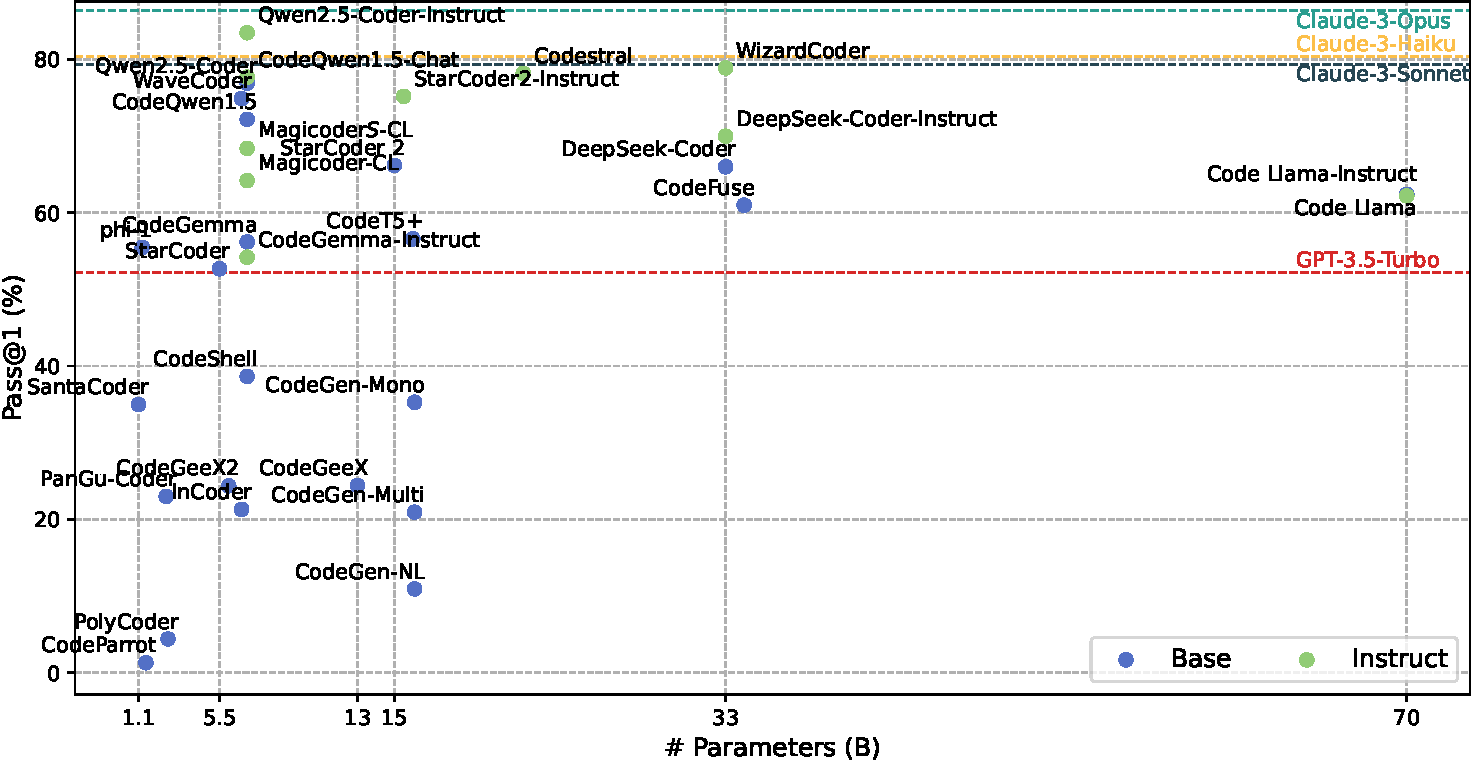
\includegraphics[width=\linewidth]{images/mbpp_scatter.pdf}
\caption{\done{The performance comparison of LLMs for code generation on the MBPP \cite{austin2021program} benchmark, measured by \texttt{Pass@1}. For models with various sizes, we report only the largest size version of each model with a magnitude of \texttt{B} parameters.} 
}
\label{fig:mbpp_performance}
\end{figure*}
% \begin{table}[t] 
% % \begin{wraptable}{R}{0.5\linewidth}
% \caption{
% % The Performance (\texttt{Pass@1}, \texttt{Pass@10}, and \texttt{Pass@100}) comparison of LLMs for code generation on HumanEval benchmark. For the model with various model size, we only report the largest size version of each model.
% \revise{The performance comparison of LLMs for code generation on the HumanEval \cite{chen2021evaluating} benchmark, measured by \texttt{Pass@1}. 
% % Due to the limitations of computational resources we faced, we directly cite the experimental results from the original papers or widely recognized open-source leaderboard in research community.
% For models with various sizes, we report only the largest size version of each model with the magnitude of \texttt{B} parameters. $^\ddag$ denotes instruction-tuned models.
% % DeepSeek-Coder-V2-Instruct is an open-source Mixture-of-Experts (MoE) code language
% % model, which has 236B parameters with only 21B activation parameters. 
% } 
% }
% \label{tab:performance_bigcodebench}
% \centering
% \scalebox{0.82}{
% \rotatebox{0}{
%     \begin{tabular}{clrc}
%     \toprule
%     & \textbf{Model} & \textbf{Size} & \texttt{Full pass@1} \\ 
% \midrule
%     \multirow{10}{*}{\textbf{Closed Source}} 
%          & GPT-4o-0513 \cite{gpt-4o} & - & 51.1 \\
%          & GPT-4-Turbo-0409 \cite{gpt-4-turbo} & - & 48.2 \\
%          & GPT-4-0613 \cite{achiam2023gpt}& - & 46  \\
%          & GPT-3.5-Turbo-0125 \cite{gpt-3.5-turbo}& - & 39.1 \\
%          & Claude-3.5-Sonnet \cite{claude3} & - & 46.8 \\
%          & Claude-3-Opus \cite{claude3} & - & 45.5 \\
%          & Claude-3-Sonnet \cite{claude3} & - & 42.7 \\
%          & Claude-3-Haiku \cite{claude3} & - & 39.4 \\
%          & Gemini-1.5-Pro \cite{reid2024gemini} & - & 43.8 \\
%          & Gemini-1.5-Flash \cite{reid2024gemini} & - & 43.5 \\
%          \midrule
%     \multirow{11}{*}{\textbf{Open Source}} 
%          & $^\ddag$Codestral \cite{codestral} & 22B & 41.8 \\
%          & $^\ddag$DeepSeek-Coder-V2-Instruct \cite{zhu2024deepseek}  & 21B (236B) & 48.2 \\
%          & $^\ddag$Qwen2.5-Coder-Instruct \cite{hui2024qwen2} & 7B & 40.4 \\
%          & $^\ddag$StarCoder2-Instruct \cite{starcoder2instruct} &  15.5B  & 37.6 \\
%          & $^\ddag$CodeGemma-Instruct \cite{codegemma_2024}  & 7B  & 32.3 \\
%          & $^\ddag$WaveCoder-Ultra \cite{yu2023wavecoder} & 6.7B & 33.9 \\
%          & $^\ddag$CodeQwen1.5-Chat \cite{codeqwen} & 7B & 39.6 \\
%          & $^\ddag$Magicoder-S-DS \cite{wei2023magicoder} & 7B & 36.2 \\
%          & $^\ddag$DeepSeek-Coder-Instruct \cite{guo2024deepseek} & 33B & 42 \\
%          & $^\ddag$Phi-3-Medium-128K-Instruct \cite{abdin2024phi} & 14B & 36.8 \\
%          & $^\ddag$Code Llama-Instruct \cite{roziere2023code} & 70B & 40.7 \\
%          & $^\ddag$CodeGeeX4 \cite{zheng2023codegeex} & 9B & 40 \\
%     \bottomrule
%     \end{tabular}
% }
% }
% \vspace{-10pt}
% % \end{wraptable}
% \end{table}

\begin{figure*}[t]
\centering
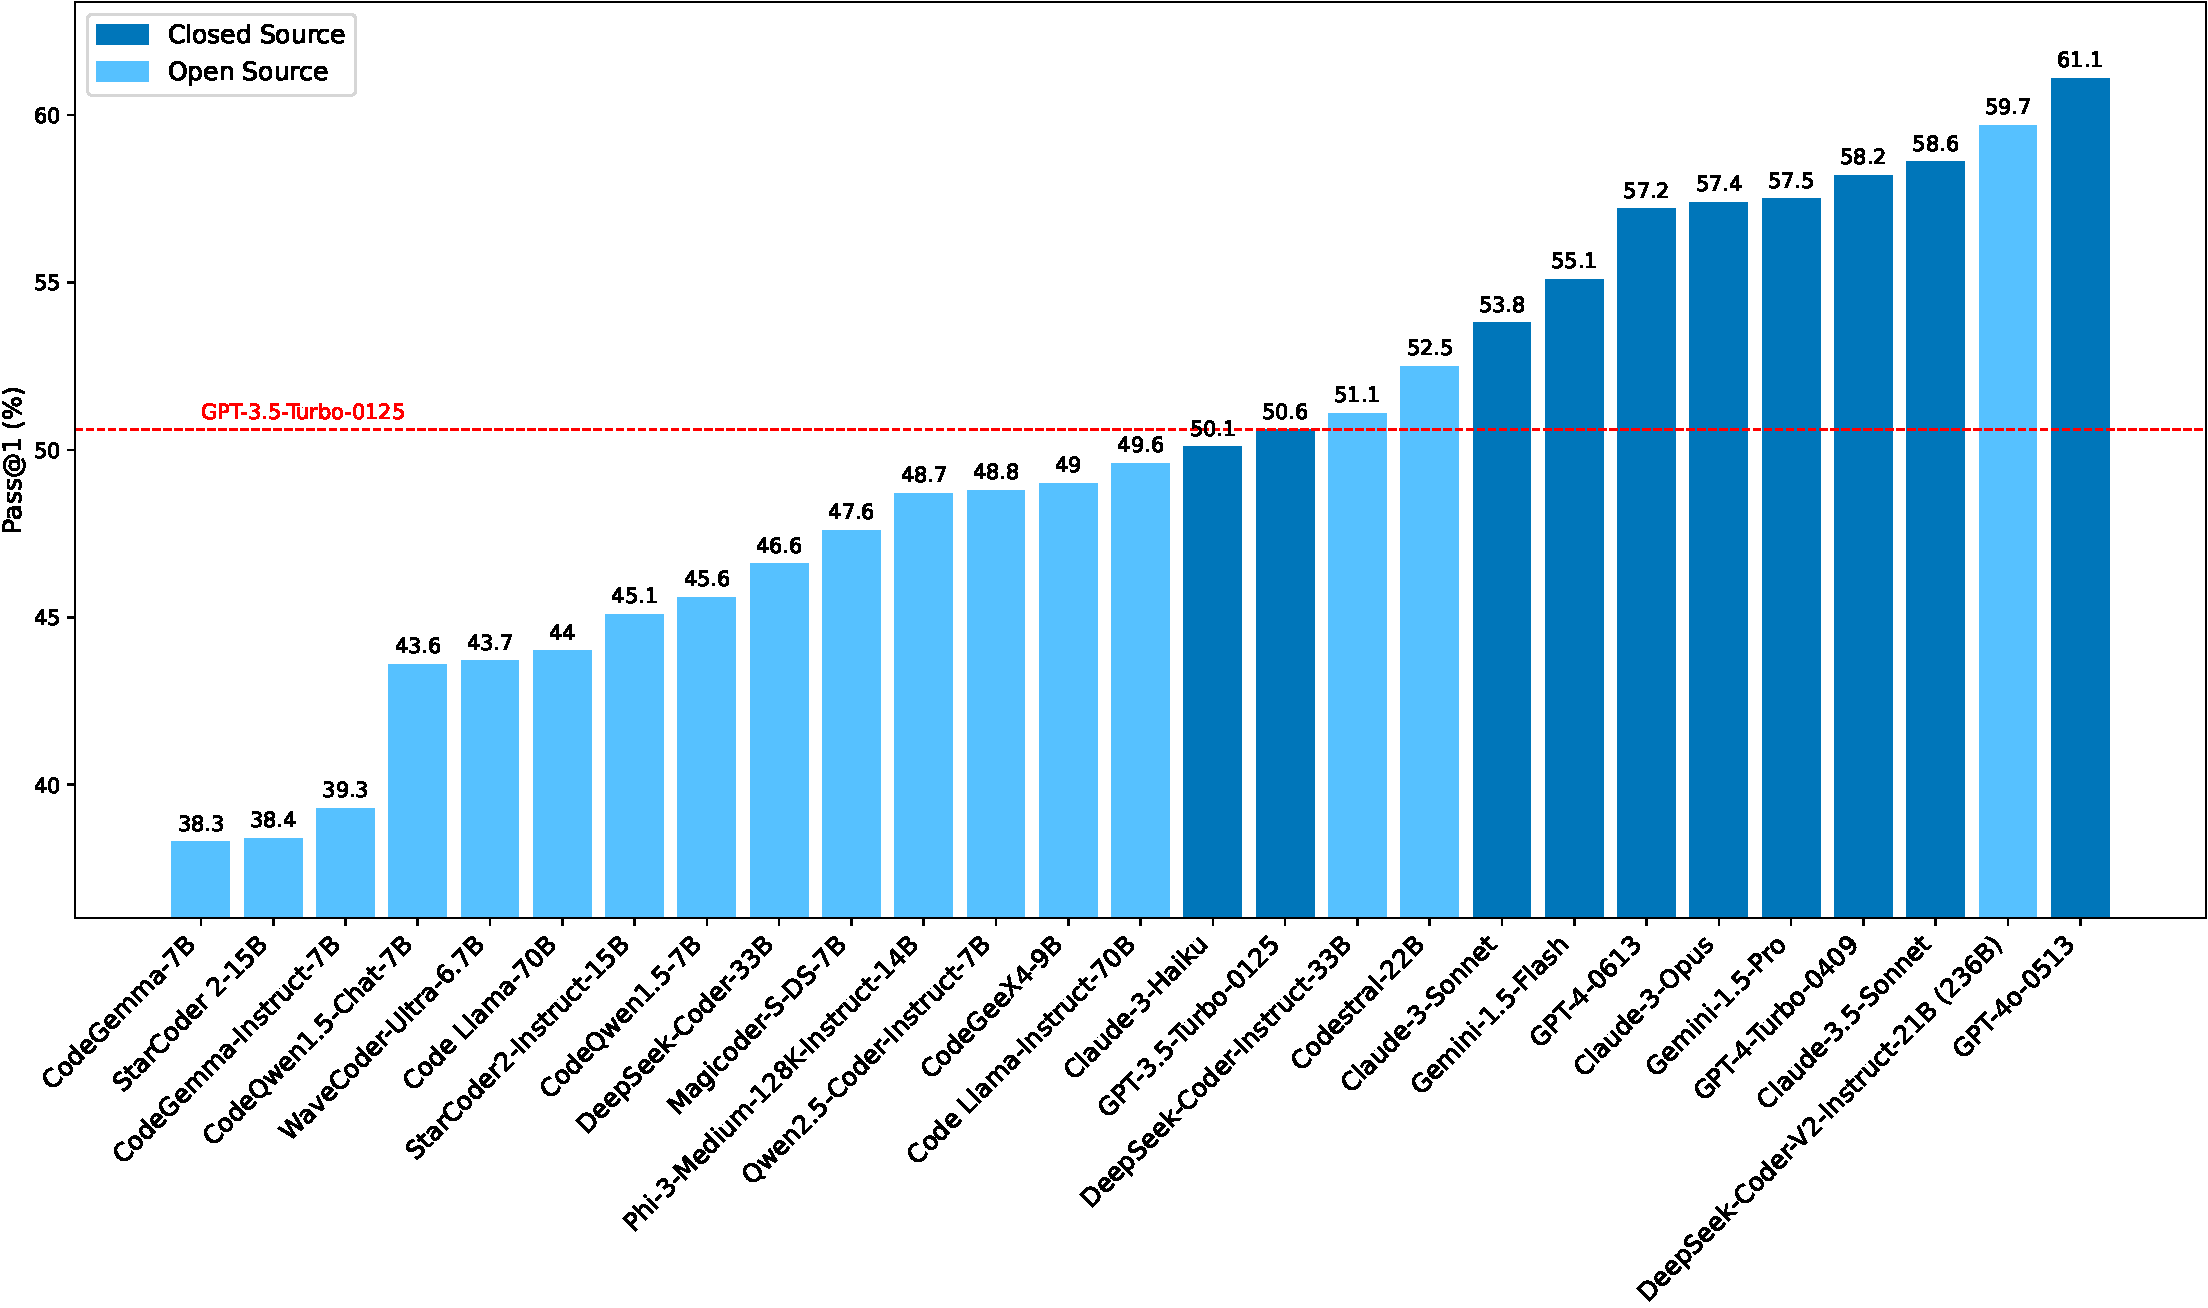
\includegraphics[width=\linewidth]{images/bigcodebench_complete_bar.pdf}
\caption{\done{The performance comparison of LLMs for code generation on the BigCodeBench \cite{zhuo2024bigcodebench} benchmark, measured by \texttt{Pass@1}. For models with various sizes, we report only the largest size version of each model with a magnitude of \texttt{B} parameters.} 
}
\label{fig:bigcodebench_performance}
\end{figure*}
% In this Section, we provide an the performance comparision of LLMs for code generaiton on the widely recognized HumanEval and MBPP benchmarks, as well as the more practical and challenging BigCodeBench benchmar, to highlight the progressive enhancements in LLM capabilities for code generation.
% These three benchmarks can be used to assess a LLM's capability in code generation from different difficulty level and scope of the programming tasks. 
% To be specific, HumanEval is more focused on complex code generation, while MBPP targets basic programming tasks, BigCodeBench focuses on practical and challenging programming tasks.
In this section, we present a performance comparison of LLMs for code generation using the well-regarded HumanEval, MBPP, and the more practical and challenging BigCodeBench benchmarks. 
This empirical comparison aims to highlight the progressive enhancements in LLM capabilities for code generation. 
These benchmarks assess an LLM's ability to generate source code across various levels of difficulty and types of programming tasks. 
Specifically, HumanEval focuses on complex code generation, MBPP targets basic programming tasks, and BigCodeBench emphasizes practical and challenging programming tasks.

% Due to the limitations of computational resources we faced, we directly cite the experimental results from the original papers or widely recognized open-source leaderboard in research community.
% We report the performance on HumanEval with the \texttt{pass@1} as shown in Table \ref{tab:performance_humaneval}, while MBPP and BigCodeBench with \texttt{pass@1}, as shown in Figure \ref{fig:mbpp_performance} and \ref{fig:bigcodebench_performance}, respectively.
Due to the limitations in computational resources we faced, we have cited experimental results from original papers or widely recognized open-source leaderboards within the research community, such as the HumanEval Leaderboard \footnote{\href{https://paperswithcode.com/sota/code-generation-on-humaneval}{https://paperswithcode.com/sota/code-generation-on-humaneval}}, EvalPlus Leaderboard \footnote{\href{https://evalplus.github.io/leaderboard.html}{https://evalplus.github.io/leaderboard.html}}, Big Code Models Leaderboard  \footnote{\href{https://huggingface.co/spaces/bigcode/bigcode-models-leaderboard}{https://huggingface.co/spaces/bigcode/bigcode-models-leaderboard}}, and BigCodeBench Leaderboard \footnote{\href{https://bigcode-bench.github.io/}{https://bigcode-bench.github.io/}}. 
We report performance on HumanEval using the \texttt{pass@1} metric, as shown in Table \ref{tab:performance_humaneval}, while MBPP and BigCodeBench results are presented with \texttt{pass@1} in Figures \ref{fig:mbpp_performance} and \ref{fig:bigcodebench_performance}, respectively.

We offer the following insights:
\begin{itemize}
    % \item The performance gap between open-source and closed-source models on three benchmarks is gradually narrowing. For example, on HumanEval benchmark, DeepSeek-Coder-V2-Instruct with only 21B activation parameters and Qwen2.5-Coder-Instruct \cite{hui2024qwen2} 7B achieves 90\% and 88.4\% pass@1 performance, respectively, which are comparable to much large closed source LLMs Claude-3.5-Sonnet with 92.0\% pass@1 performance. 
    % On MBPP benchmark, Qwen2.5-Coder-Instruct 7B with 83.5\% pass@1 significantly outperforms GPT-3.5-Turbo with 52.2\% pass@1 and achieve a very close performance compared to powerful closed-source Claude-3-Opus with 86.4\% pass@1. On more practical and challenging benchmark BigCodeBench, DeepSeek-Coder-V2-Instruct with 48.2\% surpasses all compared closed source LLMs except equal to GPT-4-Turbo-0409 with 48.2\% and lag behind GPT-4o-0513 with 51.1\%. 
    \item The performance gap between open-source and closed-source models across the three benchmarks is gradually narrowing. For instance, on the HumanEval benchmark, DeepSeek-Coder-V2-Instruct with 21B activation parameters and Qwen2.5-Coder-Instruct 7B achieve 90\% and 88.4\% pass@1, respectively. 
    These results are comparable to the much larger closed-source LLMs, such as Claude-3.5-Sonnet, which achieves 92.0\% pass@1. 
    On the MBPP benchmark, Qwen2.5-Coder-Instruct 7B with 83.5\% pass@1 significantly outperforms GPT-3.5-Turbo with 52.2\% pass@1 and closely rivals the closed-source Claude-3-Opus with 86.4\% pass@1. 
    On the BigCodeBench, DeepSeek-Coder-V2-Instruct achieves 59.7\%, surpassing all compared closed-source and open-source LLMs except for slightly falling behind GPT-4o-0513, which achieves 61.1\%.
    % \item In general, as the model parameters increase, the performance of the Code LLMs improves. However, we observe that Qwen2.5-Coder-Instruct 7B obtain 88.4 pass@1 results, outperforming StarCoder2-Instruct 15.5B with 72.6\% pass@1, DeepSeek-Coder-Instruct 33B with 79.3\% pass@1, and Code Llama-Instruct 70B with 67.8\% pass@1 by a large margin on HumanEval benchmark. We also observe consistent phonomenon across other two benchmarks. 
    % We speculate that Code LLMs with 7B parameters may be enough capable on the code generation task.
    \item Generally, as the number of model parameters increases, the performance of code LLMs improves. However, Qwen2.5-Coder-Instruct 7B achieves 88.4\% pass@1, outperforming larger models like StarCoder2-Instruct 15.5B with 72.6\% pass@1, DeepSeek-Coder-Instruct 33B with 79.3\% pass@1, and Code Llama-Instruct 70B with 67.8\% pass@1 on the HumanEval benchmark. Similar trends are observed across the other two benchmarks, suggesting that code LLMs with 7B parameters may be sufficiently capable for code generation task.
    % \item Compared to base (pretrained) models, their instruction-tuned counterpart consistently achieve better performance across all benchmarks. 
    % For example, on three benchmarks, Qwen2.5-Coder-Instruct outperforms Qwen2.5-Coder by average 21\%,  StarCoder2-Instruct improve StarCoder2 by average 50\%, CodeGemma-Instruct improve CodeGemma by average 25\%, DeepSeek-Coder-Instruct surpass DeepSeek-Coder by average 30\%, and Code Llama-Instruct improve Code Llama by average 80\%. 
    % It verifies the effectiveness of instruction tuning. However, the quality of instruction tuning dataset has significant impact on the model performance \cite{luo2023wizardcoder}.    
    % \item Instruction-tuned models consistently outperform their base (pretrained) counterparts across HumanEval and MBPP benchmarks.
    % For example, 
    % Qwen2.5-Coder-Instruct outperforms Qwen2.5-Coder by an average of 26.04\%, 
    % StarCoder2-Instruct improves StarCoder2 by an average of 35.20\%, 
    % CodeGemma-Instruct improves CodeGemma by an average of 11.26\%, 
    % DeepSeek-Coder-Instruct surpasses DeepSeek-Coder by an average of 23.71\%, and 
    % Code Llama-Instruct improves Code Llama by an average of 13.8\%. The detailed results are illustrated in Table \ref{tab:instruct_improve}.
    % This underscores the effectiveness of instruction tuning, though the quality of the instruction tuning dataset significantly impacts model performance \cite{luo2023wizardcoder,zhou2024lima}.
    \item Instruction-tuned models consistently outperform their base (pretrained) counterparts across the HumanEval and MBPP benchmarks. For instance, Qwen2.5-Coder-Instruct surpasses Qwen2.5-Coder by an average of 26.04\%, StarCoder2-Instruct improves upon StarCoder 2 by an average of 35.20\%, and CodeGemma-Instruct enhances CodeGemma by an average of 11.26\%. Additionally, DeepSeek-Coder-Instruct outperforms DeepSeek-Coder by an average of 23.71\%, while Code Llama-Instruct shows a 13.80\% improvement over Code Llama. Detailed results can be found in Table \ref{tab:instruct_improve}. These findings underscore the effectiveness of instruction tuning, although the quality of the instruction tuning dataset plays a critical role in determining model performance \cite{luo2023wizardcoder,zhou2024lima}.
    \begin{table}[t] 
% \begin{wraptable}{R}{0.5\linewidth}
\caption{\done{The performance improvement of instruction-tuned models over their pretrained counterparts on the HumanEval, MBPP, and BigCodeBench benchmarks. 
The last two rows demonstrate the average improvement on the first two benchmarks and the three benchmarks, respectively.
}
}
\label{tab:instruct_improve}
\centering
\scalebox{0.8}{
\rotatebox{0}{
    \begin{tabular}{lccccc}
    \toprule
    & \textbf{\makecell[c]{Qwen2.5-Coder-\\Instruct 7B}} & \textbf{\makecell[c]{StarCoder2-\\Instruct 15.5B}} & \textbf{\makecell[c]{CodeGemma-\\Instruct 7B}} & \textbf{\makecell[c]{DeepSeek-Coder-\\Instruct 33B}} & \textbf{\makecell[c]{Code Llama-\\Instruct 70B}} \\ 
\midrule
    \textbf{HumanEval} & 43.51\% & 56.80\% & 26.07\% & 41.35\% & 27.92\% \\
    \textbf{MBPP} & 8.58\% & 13.60\% & \cellcolor{gray!15}-3.56\% & 6.06\% & \cellcolor{gray!15}-0.32\% \\
    \textbf{BigCodeBench} & - & 17.45\% & 2.61\% & 9.66\% & 12.73\% \\
    \midrule
    \textbf{\# Avg. Imp. H. M.} & 26.04\% & 35.20\% & 11.26\%  & 23.71\% & 13.80\% \\
    \textbf{\# Avg. Imp. H. M. B.} & - & 29.28\% & 8.37\% & 19.02\% & 13.44\% \\
    \bottomrule
    \end{tabular}
}
}
% \end{wraptable}
\end{table}
    % \item The performance on HumanEval benchmark is almost saturated. However, the MBPP with basic programming tasks and BigCodeBench benchmark with more practical and challenging programming tasks requires more capable code LLMs. Besides, these benchmarks primarily focus on the functional correctness of code, they do not provide a holistic evaluation that encompasses other critical dimensions. A more comprehensive evaluation framework that integrates various aspects remains an open area for future research and development in the field of LLMs for code generation assessment.
    \item Performance on the HumanEval benchmark is nearly saturated. However, MBPP, which involves basic programming tasks, and BigCodeBench, which involves more practical and challenging programming tasks, demand more capable code LLMs. Additionally, while these benchmarks primarily evaluate the functional correctness of code, they do not provide a comprehensive assessment across other critical dimensions. Developing a more holistic evaluation framework that integrates various aspects remains an open area for future research and development in LLMs for code generation evaluation.
\end{itemize}

\textbf{Discussion}:
% Here, we discuss some of code LLMs in Table \ref{tab:performance_humaneval} to enhance clarity.
We discuss certain code LLMs in Table \ref{tab:performance_humaneval} for clarity:
% (1) For general LLMs accessed by API, they are not specifically trained on large code corpora while they achieve state-of-the-art performance in code generation. 
(1) General LLMs accessed via API are not specifically trained on large code corpora but achieve state-of-the-art performance in code generation, such as Claude-3.5-Sonnet with 92.0\% pass@1 on HumanEval benchmark.
% (2) AlphaCode targets code generation for more complex and unseen problems that require an understanding of algorithms and complex natural language, such as competitive programming problems. 
% The authors of AlphaCode found that large-scale model sampling to explore the search space, such as 1M samples per problem for CodeContests, followed by filtering based on program behavior to a small set of submissions, is critical to achieve good and reliable performance on these problems that require deeper reasoning. 
(2) AlphaCode targets code generation for more complex and unseen problems that require a deep understanding of algorithms and intricate natural language, such as those encountered in competitive programming.
The authors of AlphaCode found that large-scale model sampling to navigate the search space, such as 1M samples per problem for CodeContests, followed by filtering based on program behavior to produce a smaller set of submissions, is crucial for achieving good and reliable performance on problems that necessitate advanced reasoning.
% (3) Phi-1 1.3B is a specialized LLMs for code and trained on a selection of ``textbook quality'' data from the web (6B tokens) and synthetically generated textbooks and exercises with GPT-3.5 (1B tokens).
(3) Phi-1 1.3B is a specialized LLM for code, trained on ``textbook quality'' data from the web (6B tokens) and synthetically generated textbooks and exercises using GPT-3.5 (1B tokens).
% (4) Code Llama 70B is initialized with Llama 2 model weights and continually pre-trained on 1T tokens from a code-heavy dataset and long-context fine-tuned with an approximate 20B tokens. However, Code Llama-Instruct 70B is fine-tuned from Code Llama-Python 70B which is without long-context fine-tuning on an additional 260M tokens to better follow human instructions. 
% Surprisingly, they underperform the Code LLMs with much less parameters, such as Qwen2.5-Coder-Instruct 7B, DeepSeek-Coder-V2-Instruct 21B, and Codestral 22B across three benchmarks. The behind reason is not clear and it needs for a further exploration.  
(4) Code Llama 70B is initialized with Llama 2 model weights and continually pre-trained on 1T tokens from a code-heavy dataset and long-context fine-tuned with approximately 20B tokens. However, Code Llama-Instruct 70B is fine-tuned from Code Llama-Python 70B without long-context fine-tuning, using an additional 260M tokens to better follow human instructions. 
Surprisingly, these models underperform compared to smaller parameter Code LLMs like Qwen2.5-Coder-Instruct 7B, DeepSeek-Coder-V2-Instruct 21B, and Codestral 22B across all three benchmarks. The underlying reasons for this discrepancy remain unclear and warrant further exploration.
% (5) Different from all other open-source Code LLMs, DeepSeek-Coder-V2-Instruct is further pre-trained on DeepSeek-V2 \cite{liu2024deepseek}, which is a Mixture-of-Experts (MoE) architecture with only 21B activation parameters out of 236B parameters, with additional 6 trillion tokens with a composition of 60\% source code, 10\% math corpus, and 30\% natural language corpus. For a comprehensive understanding of MoE in LLMs, please refer to \cite{cai2024survey}.
(5) Unlike other open-source Code LLMs, DeepSeek-Coder-V2-Instruct is further pre-trained on DeepSeek-V2 \cite{liu2024deepseek}, which employs a Mixture-of-Experts (MoE) architecture with only 21B activation parameters out of 236B parameters, using an additional 6 trillion tokens composed of 60\% source code, 10\% math corpus, and 30\% natural language corpus. For a comprehensive understanding of MoE in LLMs, please refer to \cite{cai2024survey}.




}\label{sec:empirical_comparison}
%%%%%%%%%%%%%%%%%%%%%%%%%%%%%%%%%%%%%%%%%%%%%%%%%%%%%%%%%%%%%%%%%%%%%%%%
%%%%%%%%%%%%%%%%%%%%%%%%%%%%%%%%%%%%%%%%%%%%%%%%%%%%%%%%%%%%%%%%%%%%%%%%
\done{\subsection{Code LLMs Alignment}\label{sec:responsible_codeai}
% The pre-training of next-token prediction based on maximizing conditional generation probability on tremendous textual corpora endows the LLMs with world knowledge and emergency capabilities \cite{brown2020language}. 
% This training paradigm facilitates the generation of coherent and fluent text in response to various instructions.
% However, LLMs may still misunderstand human instruction that deviate from human intentions and values, generate biased content or factually incorrect information  (known as hallucination), which can limit their practical usefulness \cite{wang2023aligning,zhao2023survey,ji2023ai}.
The pre-training of LLMs for next-token prediction, aimed at maximizing conditional generation likelihood across vast textual corpora, equips these models with extensive world knowledge and emergent capabilities \cite{brown2020language}. 
This training approach enables the generation of coherent and fluent text in response to diverse instructions. 
Nonetheless, LLMs can sometimes misinterpret human instructions, produce biased content, or generate factually incorrect information (commonly referred to as hallucinations), which may limit their practical utility \cite{wang2023aligning,zhao2023survey,ji2023ai}.

% Consequently, making LLMs behave in line with human intentions and values, referred to as LLMs alignment, has emerged as a pivotal area of research \cite{ji2023ai,wang2023aligning}. 
% There are commonly-mentioned key objectives of LLMs alignment, including Robustness, Interpretability, Controllability, Ethicality, Trustworthy, Ethical, Security, Privacy, Fairness, and Safety.
% In recent years, a great efforts from LLMs researchers has been made to achieve this alignment, such as Reinforcement Learning with Human Feedback (RLHF) \cite{ouyang2022training}.
Aligning LLMs with human intentions and values, known as LLM alignment, has consequently become a critical research focus \cite{ji2023ai,wang2023aligning}. 
Key objectives frequently discussed in the context of LLM alignment include robustness, interpretability, controllability, ethicality, trustworthiness, security, privacy, fairness, and safety. 
In recent years, significant efforts have been made by researchers to achieve this alignment, employing techniques such as Reinforcement Learning with Human Feedback (RLHF) \cite{ouyang2022training}.


% However, it is not well explored to discuss the code LLMs alignment. Compared with text generation of LLMs, code generation is even more necessary to align with human values. For example, for users without any programming background, they prompt the LLMs to generate the source code and then execute it on their computer. It may potential bring catastrophic damages. To name a few, 
However, the alignment of Code LLMs has not been extensively explored. 
Compared to text generation, aligning code generation with human intentions and values is even more crucial. For instance, users without programming expertise might prompt Code LLM to generate source code and subsequently execute it on their computers, potentially causing catastrophic damage. Some potential risks include:
\begin{itemize}
    \item \textbf{Malware Infection}: The code could contain viruses, worms, or trojans that compromise our system's security.
    \item \textbf{Data Loss}: It might delete or corrupt important files and data.
    \item \textbf{Unauthorized Access}: It can create backdoors, allowing attackers to access our system remotely.
    \item \textbf{Performance Issues}: The code might consume excessive resources, slowing down our system.
    \item \textbf{Privacy Breaches}: Sensitive information, such as passwords or personal data, might be stolen.
    \item \textbf{System Damage}: It may alter system settings or damage hardware components.
    \item \textbf{Network Spread}: It could propagate across networks, affecting other devices.
    \item \textbf{Financial Loss}: If the code is ransomware, it might encrypt data and demand payment for decryption.
    \item \textbf{Legal Consequences}: Running certain types of malicious code can lead to legal repercussions.
\end{itemize} 
% As can be seen, ensuring the code LLMs alignment to generate source code aligned with human preference and values has huge significance in software development.
% Most recently, a study \cite{yang2024robustness} presents the first systematic literature review to identify seven important non-functional properties of LLM4Code beyond accuracy, including robustness, security, privacy, explainability, efficiency, and usability. This study is highly relevant to Code LLMs alignment.
% We recommend reader to refer to this survey for more details.
As illustrated, aligning Code LLMs to produce source code consistent with human preferences and values is of paramount importance in software development. A recent study \cite{yang2024robustness} provides the first systematic literature review identifying seven critical non-functional properties of LLMs for code, beyond accuracy, including robustness, security, privacy, explainability, efficiency, and usability. This study is highly pertinent to the alignment of Code LLMs. We recommend readers refer to this survey for more detailed insights.




% \done{LLMs} have exhibited remarkable instruction-following capabilities through instruction tuning. 
% However, they often produce outputs that are unexpected, toxic, biased, or hallucinated outputs that do not align with users' intentions or preferences \cite{ouyang2022training,wang2023aligning,ji2023ai}.

% In this survey, we identify five principles as the key objectives of Code LLMs alignment: Green, Responsible, Efficiency, Safety, and Trustworthy (\textbf{GREST}) from a broader perspectives.
% For each category, it involves some concepts and properties. We summarize them in the Table \ref{tab:codellm_alignment}.
% \begin{table}[t] 
\centering
\caption{\done{
Five core principles serve as the key objectives for Code LLMs alignment: Green, Responsibility, Efficiency, Safety, and Trustworthiness (collectively referred to as \textbf{GREST}).
}}
\label{tab:codellm_alignment}
\scalebox{0.65}{
\begin{tabular}{ll}
\toprule
\textbf{Principles} & \textbf{Involved Concepts and Properties} \\ 
\midrule
\textbf{Green} & 
\makecell[l]{
    %  \textbf{Energy Efficiency}: Designing systems to minimize energy consumption, reducing environmental impact and lowering financial costs.\\
    %  \textbf{Sustainable Materials}: Utilizing eco-friendly and recyclable materials in hardware and infrastructure to decrease long-term expenses. \\
    %  \textbf{Carbon Footprint}: Implementing practices to reduce emissions and offset carbon output, often leading to cost savings through efficiency. \\
    %  \textbf{Resource Optimization}: Efficient use of resources to prevent waste, promoting sustainability while reducing financial expenditures. \\
    %  \textbf{Recycling and E-Waste Management}: Ensuring proper disposal and recycling of electronic waste, which can reduce costs associated with waste management. \\
    %  \textbf{Renewable Energy}: Incorporating renewable energy sources to power operations, potentially lowering energy expenses. \\
    %  \textbf{Lifecycle Assessment}: Evaluating the environmental impact and financial costs of a product from creation to disposal to ensure sustainable practices.
     \textbf{Energy Efficiency}: Minimizing computational energy use and reduce environmental impact and financial costs.\\
     \textbf{Sustainable Materials}: Leveraging eco-friendly infrastructure and servers for code generation, lowering long-term expenses. \\
     \textbf{Carbon Footprint}: Reducing emissions associated with model training and inference to enhance efficiency and save costs. \\
     \textbf{Resource Optimization}: Efficiently utilizing computational resources to minimize waste and reduce expenses in code generation. \\
     \textbf{Recycling Management}: Responsibly dispose of hardware used in model development to reduce waste management costs. \\
     \textbf{Renewable Energy}: Utilizing renewable energy sources for powering training and inference processes to decrease energy costs.  \\
     \textbf{Lifecycle Assessment}: Evaluating the environmental and financial impacts of models from creation to deployment and disposal.
} \\
\midrule
\textbf{Responsibility} & 
\makecell[l]{
    %  \textbf{Privacy}: Protecting user data is a key responsibility. \\
    %  \textbf{Copyright Issue}: Involves responsibly handling intellectual property and others' work. \\
    %  \textbf{Explainability}: Enables users to understand the decision-making process, reflecting responsibility. \\
    %  \textbf{Usability}: Involves the system's user-friendliness as part of responsible design.
     \textbf{Ethical Considerations}: Adhering to ethical guidelines to ensure responsible use and deployment of generated code. \\
     \textbf{Accountability}: Establishing clear lines of responsibility for code generation outcomes and potential impacts. \\
     \textbf{User Education}: Providing resources and guidance to help users understand and responsibly use generated code. \\
     \textbf{Impact Assessment}: Evaluating the social and technical implications of code generation to minimize negative effects. \\
     \textbf{Regulatory Compliance}: Ensuring that generated code adheres to relevant laws (e.g., copyright) and industry regulations.
    %  \textbf{Sustainability}: Promoting environmentally conscious practices in model training and deployment to reduce carbon footprint.
} \\
\midrule
\textbf{Efficiency} & 
\makecell[l]{
     \textbf{Model Optimization}: Streamlining models to reduce computational load and improve speed. \\
     \textbf{Prompt Engineering}: Designing effective prompts to generate accurate code efficiently. \\
     \textbf{Resource Management}: Allocating computational resources wisely to balance speed and cost. \\
     \textbf{Inference Optimization}: Enhancing the inference process to quickly generate code with minimal latency. \\
     \textbf{Parallel Processing}: Utilizing parallelism to speed up code generation tasks. \\
     \textbf{Caching Mechanisms}: Implementing caching to reuse previous results and reduce redundant computations. \\
     \textbf{Evaluation Metrics}: Using precise metrics to assess and improve the efficiency of code outputs.
} \\
\midrule
\textbf{Safety} & 
\makecell[l]{
%      \textbf{Safety}: Directly relates to the system’s ability to ensure protection. \\
%      \textbf{Robustness}: Affects the system's capability to remain secure under various conditions. \\
%      \textbf{Generating Harmful or Useless Code}: Impacts the system’s safety and reliability. \\
%      \textbf{Hateful Code Comments}: Can affect the safety culture and user experience.
     \textbf{Input Validation}: Ensuring inputs (prompts) are safe and sanitized to prevent malicious exploitation. \\
     \textbf{Security Audits}: Regularly reviewing generated code for vulnerabilities and potential exploits. \\
     \textbf{Monitoring and Logging}: Keeping track of generation outputs to quickly identify and address safety issues. \\
     \textbf{User Access Control}: Limiting access to generation capabilities to trusted users to minimize risk. \\
     \textbf{Continuous Updates}: Regularly updating models with the latest safety protocols and security patches. \\
     \textbf{Ethical Guidelines}: Implementing ethical standards to guide safe and responsible code generation.
} \\
\midrule
\textbf{Trustworthiness} & 
\makecell[l]{
%      \textbf{Fairness}: Ensures the system treats all users equitably, which is fundamental to trust.\\
%      \textbf{Bias in Evaluation}: Affects the system's fairness, impacting its trustworthiness.
     \textbf{Reliability}: Ensuring that generated code consistently meets functional requirements and performs as expected. \\
     \textbf{Transparency}: Providing clear explanations of how code is generated to build user confidence. \\
     \textbf{Verification and Testing}: Using rigorous testing frameworks to ensure the generated code accuracy and reliability. \\
    % the correctness and reliability of the generated code. \\
     \textbf{Bias Mitigation}: Actively working to identify and reduce biases in code generation to ensure fairness and impartiality. \\
     \textbf{User Feedback Integration}: Continuously incorporating user feedback to refine and improve code generation processes. \\
     \textbf{Documentation}: Providing comprehensive documentation for generated code to enhance understanding and trust.
    } \\
\bottomrule
\end{tabular}
}
\end{table}
% In the following, we first define each principles and then briefly introduce a few typical works to enhance understanding.
In this survey, we identify five core principles that serve as the key objectives for aligning Code LLMs: Green, Responsibility, Efficiency, Safety, and Trustworthiness (collectively referred to as \textbf{GREST}). These principles are examined from a broader perspective. Each category encompasses various concepts and properties, which are summarized in Table \ref{tab:codellm_alignment}. 
\begin{table}[t] 
\centering
\caption{\done{
Five core principles serve as the key objectives for Code LLMs alignment: Green, Responsibility, Efficiency, Safety, and Trustworthiness (collectively referred to as \textbf{GREST}).
}}
\label{tab:codellm_alignment}
\scalebox{0.65}{
\begin{tabular}{ll}
\toprule
\textbf{Principles} & \textbf{Involved Concepts and Properties} \\ 
\midrule
\textbf{Green} & 
\makecell[l]{
    %  \textbf{Energy Efficiency}: Designing systems to minimize energy consumption, reducing environmental impact and lowering financial costs.\\
    %  \textbf{Sustainable Materials}: Utilizing eco-friendly and recyclable materials in hardware and infrastructure to decrease long-term expenses. \\
    %  \textbf{Carbon Footprint}: Implementing practices to reduce emissions and offset carbon output, often leading to cost savings through efficiency. \\
    %  \textbf{Resource Optimization}: Efficient use of resources to prevent waste, promoting sustainability while reducing financial expenditures. \\
    %  \textbf{Recycling and E-Waste Management}: Ensuring proper disposal and recycling of electronic waste, which can reduce costs associated with waste management. \\
    %  \textbf{Renewable Energy}: Incorporating renewable energy sources to power operations, potentially lowering energy expenses. \\
    %  \textbf{Lifecycle Assessment}: Evaluating the environmental impact and financial costs of a product from creation to disposal to ensure sustainable practices.
     \textbf{Energy Efficiency}: Minimizing computational energy use and reduce environmental impact and financial costs.\\
     \textbf{Sustainable Materials}: Leveraging eco-friendly infrastructure and servers for code generation, lowering long-term expenses. \\
     \textbf{Carbon Footprint}: Reducing emissions associated with model training and inference to enhance efficiency and save costs. \\
     \textbf{Resource Optimization}: Efficiently utilizing computational resources to minimize waste and reduce expenses in code generation. \\
     \textbf{Recycling Management}: Responsibly dispose of hardware used in model development to reduce waste management costs. \\
     \textbf{Renewable Energy}: Utilizing renewable energy sources for powering training and inference processes to decrease energy costs.  \\
     \textbf{Lifecycle Assessment}: Evaluating the environmental and financial impacts of models from creation to deployment and disposal.
} \\
\midrule
\textbf{Responsibility} & 
\makecell[l]{
    %  \textbf{Privacy}: Protecting user data is a key responsibility. \\
    %  \textbf{Copyright Issue}: Involves responsibly handling intellectual property and others' work. \\
    %  \textbf{Explainability}: Enables users to understand the decision-making process, reflecting responsibility. \\
    %  \textbf{Usability}: Involves the system's user-friendliness as part of responsible design.
     \textbf{Ethical Considerations}: Adhering to ethical guidelines to ensure responsible use and deployment of generated code. \\
     \textbf{Accountability}: Establishing clear lines of responsibility for code generation outcomes and potential impacts. \\
     \textbf{User Education}: Providing resources and guidance to help users understand and responsibly use generated code. \\
     \textbf{Impact Assessment}: Evaluating the social and technical implications of code generation to minimize negative effects. \\
     \textbf{Regulatory Compliance}: Ensuring that generated code adheres to relevant laws (e.g., copyright) and industry regulations.
    %  \textbf{Sustainability}: Promoting environmentally conscious practices in model training and deployment to reduce carbon footprint.
} \\
\midrule
\textbf{Efficiency} & 
\makecell[l]{
     \textbf{Model Optimization}: Streamlining models to reduce computational load and improve speed. \\
     \textbf{Prompt Engineering}: Designing effective prompts to generate accurate code efficiently. \\
     \textbf{Resource Management}: Allocating computational resources wisely to balance speed and cost. \\
     \textbf{Inference Optimization}: Enhancing the inference process to quickly generate code with minimal latency. \\
     \textbf{Parallel Processing}: Utilizing parallelism to speed up code generation tasks. \\
     \textbf{Caching Mechanisms}: Implementing caching to reuse previous results and reduce redundant computations. \\
     \textbf{Evaluation Metrics}: Using precise metrics to assess and improve the efficiency of code outputs.
} \\
\midrule
\textbf{Safety} & 
\makecell[l]{
%      \textbf{Safety}: Directly relates to the system’s ability to ensure protection. \\
%      \textbf{Robustness}: Affects the system's capability to remain secure under various conditions. \\
%      \textbf{Generating Harmful or Useless Code}: Impacts the system’s safety and reliability. \\
%      \textbf{Hateful Code Comments}: Can affect the safety culture and user experience.
     \textbf{Input Validation}: Ensuring inputs (prompts) are safe and sanitized to prevent malicious exploitation. \\
     \textbf{Security Audits}: Regularly reviewing generated code for vulnerabilities and potential exploits. \\
     \textbf{Monitoring and Logging}: Keeping track of generation outputs to quickly identify and address safety issues. \\
     \textbf{User Access Control}: Limiting access to generation capabilities to trusted users to minimize risk. \\
     \textbf{Continuous Updates}: Regularly updating models with the latest safety protocols and security patches. \\
     \textbf{Ethical Guidelines}: Implementing ethical standards to guide safe and responsible code generation.
} \\
\midrule
\textbf{Trustworthiness} & 
\makecell[l]{
%      \textbf{Fairness}: Ensures the system treats all users equitably, which is fundamental to trust.\\
%      \textbf{Bias in Evaluation}: Affects the system's fairness, impacting its trustworthiness.
     \textbf{Reliability}: Ensuring that generated code consistently meets functional requirements and performs as expected. \\
     \textbf{Transparency}: Providing clear explanations of how code is generated to build user confidence. \\
     \textbf{Verification and Testing}: Using rigorous testing frameworks to ensure the generated code accuracy and reliability. \\
    % the correctness and reliability of the generated code. \\
     \textbf{Bias Mitigation}: Actively working to identify and reduce biases in code generation to ensure fairness and impartiality. \\
     \textbf{User Feedback Integration}: Continuously incorporating user feedback to refine and improve code generation processes. \\
     \textbf{Documentation}: Providing comprehensive documentation for generated code to enhance understanding and trust.
    } \\
\bottomrule
\end{tabular}
}
\end{table}
In the following, we define each principle and briefly introduce a few notable works to enhance understanding.

\textbf{Green}: 
% Green principle emphasizes the importance of environmental sustainability in the development and deployment of LLMs for code generation. 
% It generally involves optimizing energy consumption, reducing the carbon footprint and financial costs during training and inference. 
The Green principle underscores the importance of environmental sustainability in the development and deployment of LLMs for code generation. This involves optimizing energy consumption and reducing both the carbon footprint and financial costs associated with training and inference processes.
% However, current (Code) LLMs training, inference, and deployment are an extremely resource-intensive process. For example, training GPT-3 with 175 billion parameters, required 355 years of single-processor computing time and consumed 284,000 kWh of energy, and estimates of 552.1 tons of CO$_2$ \cite{samsi2023words}.
% What's more, a ChatGPT-like application with estimated use of 11 million requests/hour produces emissions of 12.8k metric tons of CO2/year, 25 times the carbon emissions for training GPT-3 \cite{chien2023reducing}. 
Currently, training, inference, and deployment of Code LLMs are notably resource-intensive. For example, training GPT-3, with its 175 billion parameters, required the equivalent of 355 years of single-processor computing time and consumed 284,000 kWh of energy, resulting in an estimated 552.1 tons of CO$_2$ emissions \cite{samsi2023words}. 
Furthermore, a ChatGPT-like application, with an estimated usage of 11 million requests per hour, can produce emissions of 12.8k metric tons of CO$_2$ per year, which is 25 times the carbon emissions associated with training GPT-3 \cite{chien2023reducing}.
% To mitigate these costs, techniques such as specialized hardware development (e.g., TPUs (Tensor Processing Units) and NPUs (neural processing units)), model compression (e.g., quantization and knowledge distillation), parameter-efficient fine-tuning (PEFT), and renewable energy sources are often employed to adhere to this principle.
To mitigate these costs, several techniques are often employed, such as the development of specialized hardware (e.g., Tensor Processing Units (TPUs) and Neural Processing Units (NPUs)), model compression methods (e.g., quantization and knowledge distillation), parameter-efficient fine-tuning (PEFT), and the use of renewable energy sources.
% For example, Shi et al. \cite{shi2024greening} use knowledge distillation to reduce the size of CodeBERT \cite{feng2020codebert} and GraphCodeBERT \cite{guo2020graphcodebert} to a optimized models with 3MB, which is $160\times$ smaller than the original large models, and significantly reduce the energy consumption (up to $184\times$ less) and carbon footprint (up to $157\times$ less).
% Wei et al. \cite{wei2023towards} utilize quantization technique for Code LLMs (CodeGen \cite{nijkamp2022codegen} and Incoder \cite{fried2022incoder}) parameters with lower-bit integer (e.g., \texttt{int8}), which makes Code LLMs reduce storage by 67.3\% to 70.8\%, carbon footprint by 28.8\% to 55.0\%, and pricing cost by 28.9\% to 55\%. 
For instance, Shi et al. \cite{shi2024greening} applied knowledge distillation to reduce the size of CodeBERT \cite{feng2020codebert} and GraphCodeBERT \cite{guo2020graphcodebert}, resulting in optimized models of just 3MB. These models are 160 times smaller than the original large models and significantly reduce energy consumption by up to 184 times and carbon footprint by up to 157 times. Similarly, Wei et al. \cite{wei2023towards} utilized quantization techniques for Code LLMs such as CodeGen \cite{nijkamp2022codegen} and Incoder \cite{fried2022incoder} by employing lower-bit integers (e.g., \texttt{int8}). This approach reduced storage requirements by 67.3\% to 70.8\%, carbon footprint by 28.8\% to 55.0\%, and pricing costs by 28.9\% to 55.0\%.

\textbf{Responsibility}: 
% Responsible principle emphasizes ethical considerations, fairness, and accountability throughout the lifecycle of (Code) LLMs. 
% This includes addressing biases in training data, ensuring fairness and transparency in model decision-making, maintaining accountability for outputs, adhering to relevant laws (e.g., copyright), implementing mechanisms to prevent misuse, and clear communication regarding the model's capabilities and limitations.
The Responsibility principle in the context of Code LLMs underscores the importance of ethical considerations, fairness, and accountability throughout their lifecycle. This involves addressing biases in training data, ensuring fairness and transparency in model decision-making, maintaining accountability for outputs, adhering to applicable laws (e.g., copyright), implementing safeguards against misuse, and providing clear communication about the model's capabilities and limitations.
Specifically, 
\begin{itemize}
    % (1) biases in code generation can lead to flawed software or reinforce stereotypes, which can have significant societal impacts. 
    % For instance, if an LLM used for generating code inherits biases from its training data, it might produce software that inadvertently discriminates against certain user groups. 
    % This can result in applications that do not cater to the diverse needs of users, leading to exclusionary practices and reinforcing existing stereotypes \cite{mouselinos2022simple,liu2023uncovering}. 
    \item \textit{Bias Mitigation}. Biases in code generation can lead to flawed software and reinforce stereotypes, potentially causing significant societal impacts. For example, an Code LLM that inherits biases from its training data may produce source code/software that inadvertently discriminates against certain user groups. This can result in applications that fail to meet the diverse needs of users, promoting exclusionary practices and reinforcing existing stereotypes \cite{mouselinos2022simple,liu2023uncovering}.
    % (2) A lack of fairness and transparency in decision-making with LLMs for code generation can lead to biased or suboptimal code solutions. If the model's decision-making process is opaque, developers might inadvertently introduce code that favors certain frameworks or libraries, limiting innovation and diversity in software development. This lack of transparency can lead to unfair advantages and hinder collaborative efforts in tech communities \cite{bogina2022educating}.
    \item \textit{Fairness and Transparency}. A lack of fairness and transparency in Code LLM decision-making can result in biased or suboptimal code solutions. If the model's decision-making process is opaque, developers might unknowingly introduce code that favors specific frameworks or libraries, thereby limiting innovation and diversity in software development. This opacity can create unfair advantages and hinder collaborative efforts within tech communities \cite{bogina2022educating}.
    % (3) Adhering to relevant laws, such as license and copyright, is essential when using LLMs for code generation to avoid legal complications and determine whether the code generated by LLMs can be actually used in practice or not. 
    % If an LLM generates code snippets that inadvertently infringe on existing copyrights, it can lead to legal disputes and financial liabilities for developers and organizations \cite{xu2024first}. 
    % This can hinder innovation by discouraging the use of advanced AI tools due to fear of legal repercussions, thus affecting the broader tech community's growth and collaboration.
    \item \textit{Legal Compliance}. Compliance with relevant laws, such as licensing and copyright, is crucial when using Code LLMs for code generation to avoid legal complications. If an Code LLM generates code snippets that inadvertently infringe on existing copyrights, it can lead to legal disputes and financial liabilities for developers and organizations \cite{xu2024first}. Such risks may discourage the use of advanced AI tools, thus stifling innovation and affecting growth and collaboration within the tech community.
    % (4) Without accountability for the code generated by LLMs, it becomes difficult to address bugs or security vulnerabilities. If a model generates faulty code that leads to a security breach, the absence of clear accountability could result in significant financial and reputational damage for companies. This uncertainty in responsibility can delay the resolution of critical issues and impede trust in AI-assisted development \cite{liesenfeld2023opening}.
    \item \textit{Accountability}. Without accountability for code generated by Code LLMs, addressing bugs or security vulnerabilities becomes challenging. If a model generates faulty code leading to a security breach, the absence of clear accountability can result in significant financial and reputational damage for companies. This uncertainty can delay critical issue resolution and impede trust in AI-assisted development \cite{liesenfeld2023opening}.
    % (5) Failing to implement mechanisms to prevent misuse of code generation models can allow for the creation of harmful software. For instance, models could be exploited to generate malware or unauthorized scripts, posing risks to cybersecurity. Without safeguards, these models can facilitate malicious activities, threatening both individual and organizational security \cite{mousavi2024investigation}.
    \item \textit{Misuse Prevention}. Failing to implement mechanisms to prevent the misuse of Code LLMs can enable the creation of harmful software. For example, models could be exploited to generate malware or unauthorized scripts, posing cybersecurity risks. Without proper safeguards, these models can facilitate malicious activities, threatening both individual and organizational security \cite{mousavi2024investigation}.
    % (6) Without clear communication about a model's capabilities and limitations in code generation, developers may misuse the model or overestimate its abilities. For example, relying on the model to generate complex, mission-critical code without human oversight could lead to significant software failures. Misunderstanding its limitations can result in faulty implementations and lost productivity \cite{ross2023programmer}.
    \item \textit{Clear Communication}. Without clear communication about a model's capabilities and limitations, developers may misuse the model or overestimate its abilities. Relying on the model to generate complex, mission-critical code without human oversight can lead to significant software failures. Misunderstanding its limitations can result in faulty implementations and lost productivity \cite{ross2023programmer}.
\end{itemize}
% Potential mitigation methods such as bias detection and mitigation, quantification and evaluation, and ethical guidelines are essential to adhere to this principle. 
% Liu et al. \cite{liu2023uncovering} propose a new paradigm to construct code prompts and successfully uncover social biases in code generation models, and develop a dataset along with three metrics to evaluate the overall social bias.
% Most recently, Xu et al. \cite{xu2024first} propose an evaluation benchmark LiCoEval, to evaluate the license compliance capabilities of LLMs.
% Additionally, incorporating diverse perspectives in the development teams and engaging with stakeholders from various communities can further align Code LLM outputs with ethical standards and societal values.
To adhere to this principle, potential mitigation methods include bias detection and mitigation, quantification and evaluation, and adherence to ethical guidelines. 
Liu et al. \cite{liu2023uncovering} propose a new paradigm for constructing code prompts, successfully uncovering social biases in code generation models, and developing a dataset along with three metrics to evaluate overall social bias. 
Recently, Xu et al. \cite{xu2024first} introduced LiCoEval, an evaluation benchmark for assessing the license compliance capabilities of LLMs. Additionally, incorporating diverse perspectives in development teams and engaging with stakeholders from various communities can further align Code LLM outputs with ethical standards and societal values.


\textbf{Efficiency}: 
% Efficiency principle focuses on maximizing the performance and speed of LLMs for code generation while minimizing computational resources for model training and inference.
% For example, GPT-3 with 175 billion parameters requires very high resources in training, which takes around 1,024 NVIDIA V100 GPUs and costing around 4.6M and 34 days to train the model. 
% Various model compression (e.g., pruning, quantization, and knowledge distillation), optimized algorithms (e.g., AdamW), parallel strategies (e.g, tensor, pipeline, and data parallelism), and parameter-efficient fine-tuning (see Section \ref{sec:peft}) are often employed to achieve this goal.
% For the comprehensive and detailed methods to enhance efficiency of LLMs for code generation, please refer to the Section 4.5.2 Efficiency Enhancement in \cite{yang2024robustness}.
The Efficiency principle emphasizes optimizing the performance and speed of Code LLMs for code generation while minimizing the computational resources required for training and inference. 
For instance, training the GPT-3 model, which consists of 175 billion parameters, demands substantial resources. It requires approximately 1,024 NVIDIA V100 GPUs, costing around $4.6$ million and taking approximately 34 days to complete the training process. 
To address these challenges, various techniques are employed, including model compression methods such as pruning, quantization, and knowledge distillation. Additionally, optimized algorithms like AdamW, parallel strategies such as tensor, pipeline, and data parallelism, and parameter-efficient fine-tuning (PEFT) (see Section \ref{sec:peft}) are often utilized. 
For a comprehensive and detailed discussion on methods to enhance the efficiency of Code LLMs for code generation, please refer to Section 4.5.2, ``Efficiency Enhancement'', in \cite{yang2024robustness}.

\textbf{Safety}: 
% Safety principle involves rigorous testing and validation processes to detect and mitigate risks associated with generated code by LLMs. 
% Ensuring the safety of LLMs in code generation is paramount, as these models can potentially introduce vulnerabilities, errors, or privacy information into software systems.
The Safety principle of Code LLMs is of utmost importance due to their potential to introduce vulnerabilities, errors, or privacy breaches into software systems. 
Ensuring safety involves comprehensive testing and validation processes to detect and mitigate these risks.
% For example, attackers can manipulate the training process of LLMs by injecting poisoned examples into the training data known as data poisoning attacks to let model produce undesired/vulnerable/error code \cite{schuster2021you}. 
% When attackers can not access the training process, Hajipour et al. \cite{hajipour2024codelmsec} introduce a black-box inversion approach based on few-shot prompting, which finds relevant prompts that lead black-box code generation models to generate vulnerable code.
% Moreover, Yang et al. \cite{yang2024unveiling} and Al-Kaswan et al. \cite{al2024traces} find that Code LLMs (like CodeParrot \cite{codeparrot}) can potential memorize its training data to produce personally identifiable information like emails, names, IP addresses, highlighting the privacy leakage risks. 
% Yuan et al. \cite{yuan2023gpt} discover that chat with ChatGPT and GPT-4 in cipher (non-natural language) can bypass the safety alignment techniques of LLMs, leading to unsafe behaviors, like "stealing money from the bank". 
For instance, attackers might compromise the training process of LLMs by injecting malicious examples into the training data, a method known as data poisoning attacks \cite{schuster2021you}. 
Even when attackers lack access to the training process, they may employ techniques like the black-box inversion approach introduced by Hajipour et al. \cite{hajipour2024codelmsec}. This method uses few-shot prompting to identify prompts that coax black-box code generation models into producing vulnerable code. 
Furthermore, Yang et al. \cite{yang2024unveiling} and Al-Kaswan et al. \cite{al2024traces} reveals that Code LLMs, such as CodeParrot \cite{codeparrot}, can memorize training data, potentially outputting personally identifiable information like emails, names, and IP addresses, thereby posing significant privacy risks. Additionally, Yuan et al. \cite{yuan2023gpt} demonstrate that engaging with ChatGPT and GPT-4 in non-natural languages can circumvent safety alignment measures, leading to unsafe outcomes, such as ``The steps involved in stealing money from a bank.''.
% To enhance the safety of LLMs for code generation, detecting and removing the privacy information contained in training data is the prevalent way. 
% For example,  \cite{fried2022incoder} and \cite{allal2023santacoder} carefully design regular expressions to identify all the privacy information in the training data and remove it. 
% Moreover, to defend against black-box inversion, it is advisable to implement prompt filtering mechanisms to identify and block prompts that may lead to the generation of insecure code. 
% Additionally, employing adversarial training techniques can enhance the model's resilience against malicious prompts. 
% Utilizing reinforcement learning techniques can further align Code LLMs with human preferences, reducing the likelihood of harmful outputs.
To bolster the safety of LLMs in code generation, it is crucial to detect and eliminate privacy-related information from training datasets. 
For example, approaches outlined in \cite{fried2022incoder} and \cite{allal2023santacoder} utilize carefully crafted regular expressions to identify and remove private information from training data. 
To counteract black-box inversion, implementing prompt filtering mechanisms is recommended to identify and block prompts that might result in insecure code generation. 
Moreover, adversarial training can enhance the model's resilience to malicious prompts. Employing reinforcement learning methods can further align Code LLMs with human preferences, thereby reducing the likelihood of producing harmful outputs.

\textbf{Trustworthiness}: 
% Trustworthy principle revolves around creating models that users can rely on for accurate and reliable outputs, which is essential for their acceptance and widespread use.  
% This involves ensuring model transparency, providing explanations for decisions, and maintaining consistent performance across various scenarios.
The Trustworthiness principle focuses on developing Code LLMs that users can depend on for accurate and reliable code generation, which is crucial for their acceptance and widespread adoption. 
Achieving this requires ensuring model transparency, providing explanations for decisions, and maintaining consistent performance across various scenarios.
% For example, Ji et al. \cite{ji2023benchmarking} propose a causal graph-based representation of the prompt and the generated code to identify the causal relations between the prompt and the derived code. Thus, it provides insights into LLM effectiveness, and aid end-users in understanding predictions. 
% Palacio et al. \cite{palacio2023evaluating} propose ASTxplainer, which extracts and aggregate normalized model logits within AST structures to align token predictions with AST nodes, to provide visualizations of LLM predictions that aid end-users in understanding model predictions.  
% Therefore, by prioritizing trustworthiness, it can enhance user confidence and facilitate the integration of LLMs into diverse coding environments.
For instance, Ji et al. \cite{ji2023benchmarking} propose a causal graph-based representation of prompts and generated code to identify the causal relationships between them. This approach offers insights into the effectiveness of Code LLMs and assists end-users in understanding the generation. 
Similarly, Palacio et al. \cite{palacio2023evaluating} introduce ASTxplainer, a tool that extracts and aggregates normalized model logits within Abstract Syntax Tree (AST) structures. This alignment of token predictions with AST nodes provides visualizations that enhance end-user understanding of Code LLM predictions.
Therefore, by prioritizing trustworthiness, we can bolster user confidence and facilitate the integration of Code LLMs into diverse coding environments.
% By adhering to above-mentioned five principles as the key objectives of Code LLMs alignment, researchers and developers can build LLMs for code generation that are not only powerful but also ethical, sustainable, and user-centric.
By adhering to the aforementioned principles as key objectives for aligning Code LLMs, researchers and developers can create LLMs for code generation that are not only capable but also ethical, sustainable, and user-centric.







}\label{sec:grest_llm4code}

% These models are now integral to a myriad of applications, demonstrating proficiency in areas such as text generation, translation, and image recognition.
%%%%%%%%%%%%%%%%%%%%%%%%%%%%%%%%%%%%%%%%%%%%%%%%%%%%%%%%%%%%%%%%%%%%%%%%
%%%%%%%%%%%%%%%%%%%%%%%%%%%%%%%%%%%%%%%%%%%%%%%%%%%%%%%%%%%%%%%%%%%%%%%%
\begin{table}[p!]
\caption{The overview of code assistant applications powered by \done{LLMs}. The column labeled `\textbf{PLs}' and `\textbf{IDEs}' indicate programming languages and integrated development environments, respectively \cite{zan2023large}.}
\label{tab:products}
\centering
\scalebox{0.71}{
\rotatebox{270}{
    \begin{tabular}{llllll} 
        \toprule
        \textbf{Institution} & \textbf{Products} & \textbf{Model} & \textbf{Supported Features} & \textbf{Supported PLs} & \textbf{Supported IDEs} \\ 
        \toprule
        GitHub \& OpenAI & GitHub Copilot \cite{chen2021evaluating} & Codex & 
        \begin{tabular}[c]{@{}l@{}} Code Completions, Code Generation, \\
        Coding Questions Answering,\\ Code Refactoring, Code Issues Fix, \\Unit Test Cases Generation, \\Code Documentation Generation\end{tabular} &
        \begin{tabular}[c]{@{}l@{}}Java, Python, JavaScript, TypeScript,\\Perl,~R,~PowerShell, Rust,~SQL,~CSS,~\\Ruby,  Julia,~C\#,~PHP,~Swift,~C++,Go,\\HTML, JSON, SCSS,~.NET, Less,\\T-SQL, Markdown\end{tabular} & 
        \begin{tabular}[c]{@{}l@{}}Visual Studio, VS Code,~Neovim,\\JetBrains IDE\end{tabular}  \\ 
        \midrule
        Zhipu AI & CodeGeeX \cite{zheng2023codegeex} & CodeGeeX & 
        \begin{tabular}[c]{@{}l@{}} Code Generation, Code Translation, \\Code Completion, Code Interpretation, \\Code Bugs Fix, Comment Generation, \\AI Chatbot\end{tabular} &
        \begin{tabular}[c]{@{}l@{}}PHP, Go,~C,~C\#,~C++,~Rust,~Perl, CSS,\\Java, Python, JavaScript, TypeScript, \\Objective C++, Objective C, Pascal,\\HTML, SQL,~Kotlin,~R, Shell, Cuda,\\Fortran, Tex, Lean,~Scala\end{tabular} & 
        \begin{tabular}[c]{@{}l@{}}Clion, RubyMine, AppCode,~Aqua,\\IntelliJ IDEA, VS Code, PyCharm,\\Android Studio, WebStorm,~Rider,\\GoLand, DataGrip, DataSpell\end{tabular} \\ 
        \midrule
        Amazon & CodeWhisperer \cite{CodeWhisperer} & $-$ & 
        \begin{tabular}[c]{@{}l@{}} Code Completion, Code Explanation, \\ Code Translation, \\
        Code Security Identification, \\ Code Suggestion \end{tabular} &
        \begin{tabular}[c]{@{}l@{}}Java, Python, TypeScript, JavaScript,\\C\#\end{tabular} & 
        \begin{tabular}[c]{@{}l@{}}JetBrains IDE, VS Code, AWS Cloud9,\\AWS Lambda\end{tabular} \\
        \midrule
        Codeium & Codeium \cite{Codeium} & $-$ & 
        \begin{tabular}[c]{@{}l@{}} Code Completion, Bug Detection,\\Code Suggestions, AI Chatbot,\\Test Type Generation,\\Test Plan Creation,\\
        Codebase Search\end{tabular} &
        \begin{tabular}[c]{@{}l@{}} More than 70 languages in total,\\
        including but not limited to:\\
        C, C\#, C++, Dart, CSS, Go, Elixir,\\HTML, Haskell, Julia, Java, JavaScript,\\Lisp, Kotlin, Lua, Objective-C,\\Perl, Pascal, PHP, Protobuf,\\R, Python, Ruby, Scala, Rust,\\Swift, SQL, TS, Vue\end{tabular} & 
        \begin{tabular}[c]{@{}l@{}} JetBrains, VSCode, Visual Studio,\\Colab, Jupyter, Deepnote,\\Notebooks, Databricks, Chrome,\\Vim, Neovim, Eclipse, Emacs,\\
        VSCode Web IDEs, Sublime Text\end{tabular} \\
        \midrule
        Huawei & CodeArts Snap \cite{shen2023pangu} & PanGu-Coder &
        \begin{tabular}[c]{@{}l@{}}Code Generation, Code Explanation\\ Research and Development Knowledge\\ Question and Answer\\ Code Comment, Code Debug \\Unit Test Case Generation \end{tabular} &
        \begin{tabular}[c]{@{}l@{}}Java, Python \end{tabular} & 
        \begin{tabular}[c]{@{}l@{}}PyCharm, VS Code, IntelliJ \end{tabular} \\
        \midrule
        Tabnine & TabNine \cite{TabNine} & $-$ & 
        \begin{tabular}[c]{@{}l@{}}Code Generation, Code Completion,\\Code Explanation, Bug Fix,\\
        Code Recommendation, Code Refactoring,\\
        Code Test Generation,\\Docstring Generation\end{tabular} &
        \begin{tabular}[c]{@{}l@{}}Python, Javascript, Java, TypeScript,\\HTML, Haskell, Matlab, Kotlin, Sass,\\Go, PHP, Ruby, C, C\#, C++,~Swift,~\\Rust,~CSS,~Perl,~Angular, Dart, React,\\Objective C, NodeJS, Scala,~\end{tabular} & 
        \begin{tabular}[c]{@{}l@{}}Sublime, PyCharm, Neovim,~Rider,\\VS Code, IntelliJ IDE, Visual Studio,\\PhpStorm, Vim, RubyMine,~DataGrip,\\Android Studio, WebStorm,~Emacs,\\Clion, Jupyter Notebook,~JupyterLab,\\Eclipse,~GoLand, AppCode\end{tabular}  \\ 
        \midrule
        Replit & Replit\cite{Replit} & replit-code & 
        \begin{tabular}[c]{@{}l@{}} Code Completion, Code Editing,\\Code Generation, Code Explanation,\\
        Code Suggestion, Code Test Generation\end{tabular} &
        \begin{tabular}[c]{@{}l@{}} C\#, Bash, C, CSS, C++, Java, Go,\\HTML, JavaScript, Perl, PHP,\\
        Ruby, Python, R, SQL, Rust\end{tabular} & 
        \begin{tabular}[c]{@{}l@{}} $-$\end{tabular} \\
        % \midrule
        % & aiXcoder & $-$ & 
        % \begin{tabular}[c]{@{}l@{}}~\end{tabular} &
        % \begin{tabular}[c]{@{}l@{}}Python, Java, JavaScript, Typescript, \\Go, PHP, C, C++\end{tabular} & 
        % \begin{tabular}[c]{@{}l@{}}VS Code, IntelliJ IDEA, PyCharm,~\\STS3,~WebStorm,~Rider, Clion, STS4\\Android Studio,~PhpStorm, Eclipse,\\GoLand\end{tabular} \\ 
        % \midrule
        % & IntelliCode & $-$ & 
        % \begin{tabular}[c]{@{}l@{}}~\end{tabular} &
        % \begin{tabular}[c]{@{}l@{}}Python, Java, JavaScript, TypeScript, \\C\#, C++, SQL Server, XAML\end{tabular} & VS Code, Visual Studio \\ 
        \bottomrule
    \end{tabular}
}
}
\end{table}
\begin{figure*}[t]
\centering
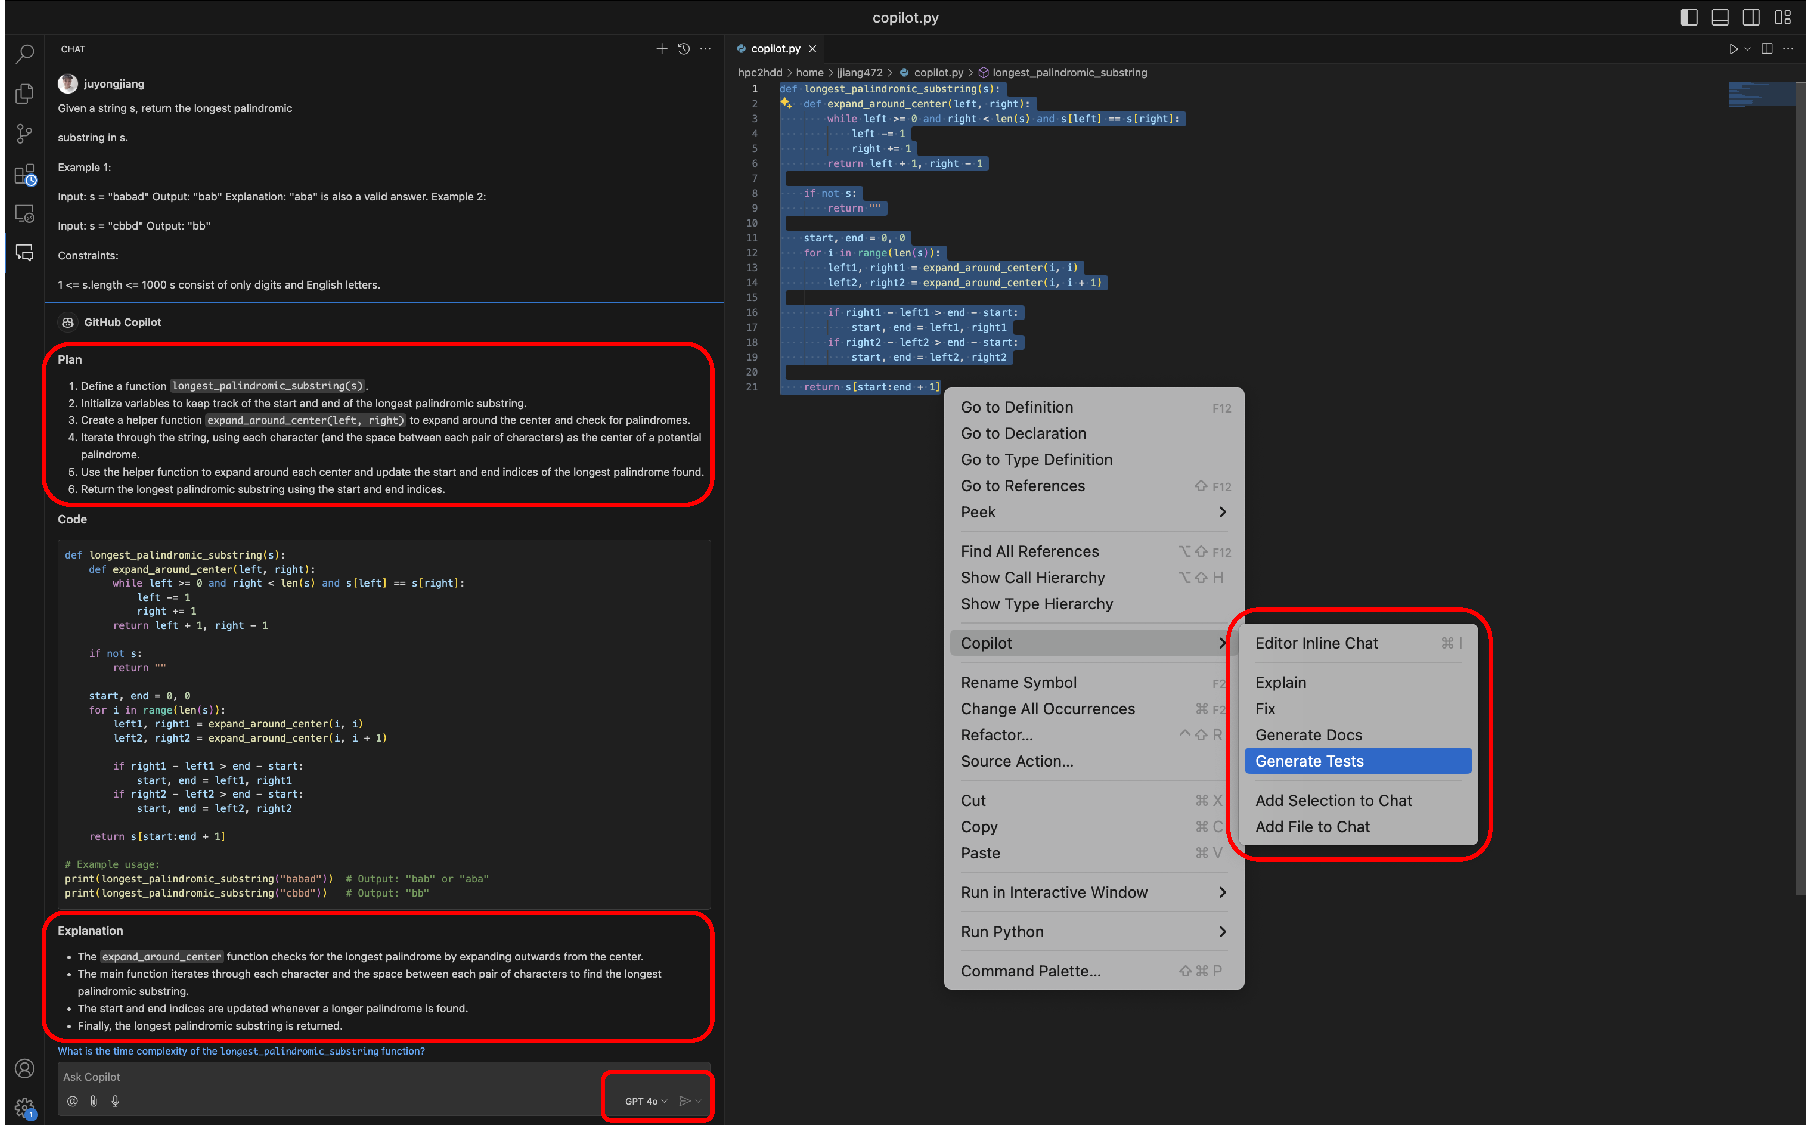
\includegraphics[width=0.95\linewidth]{images/Copilot.pdf}
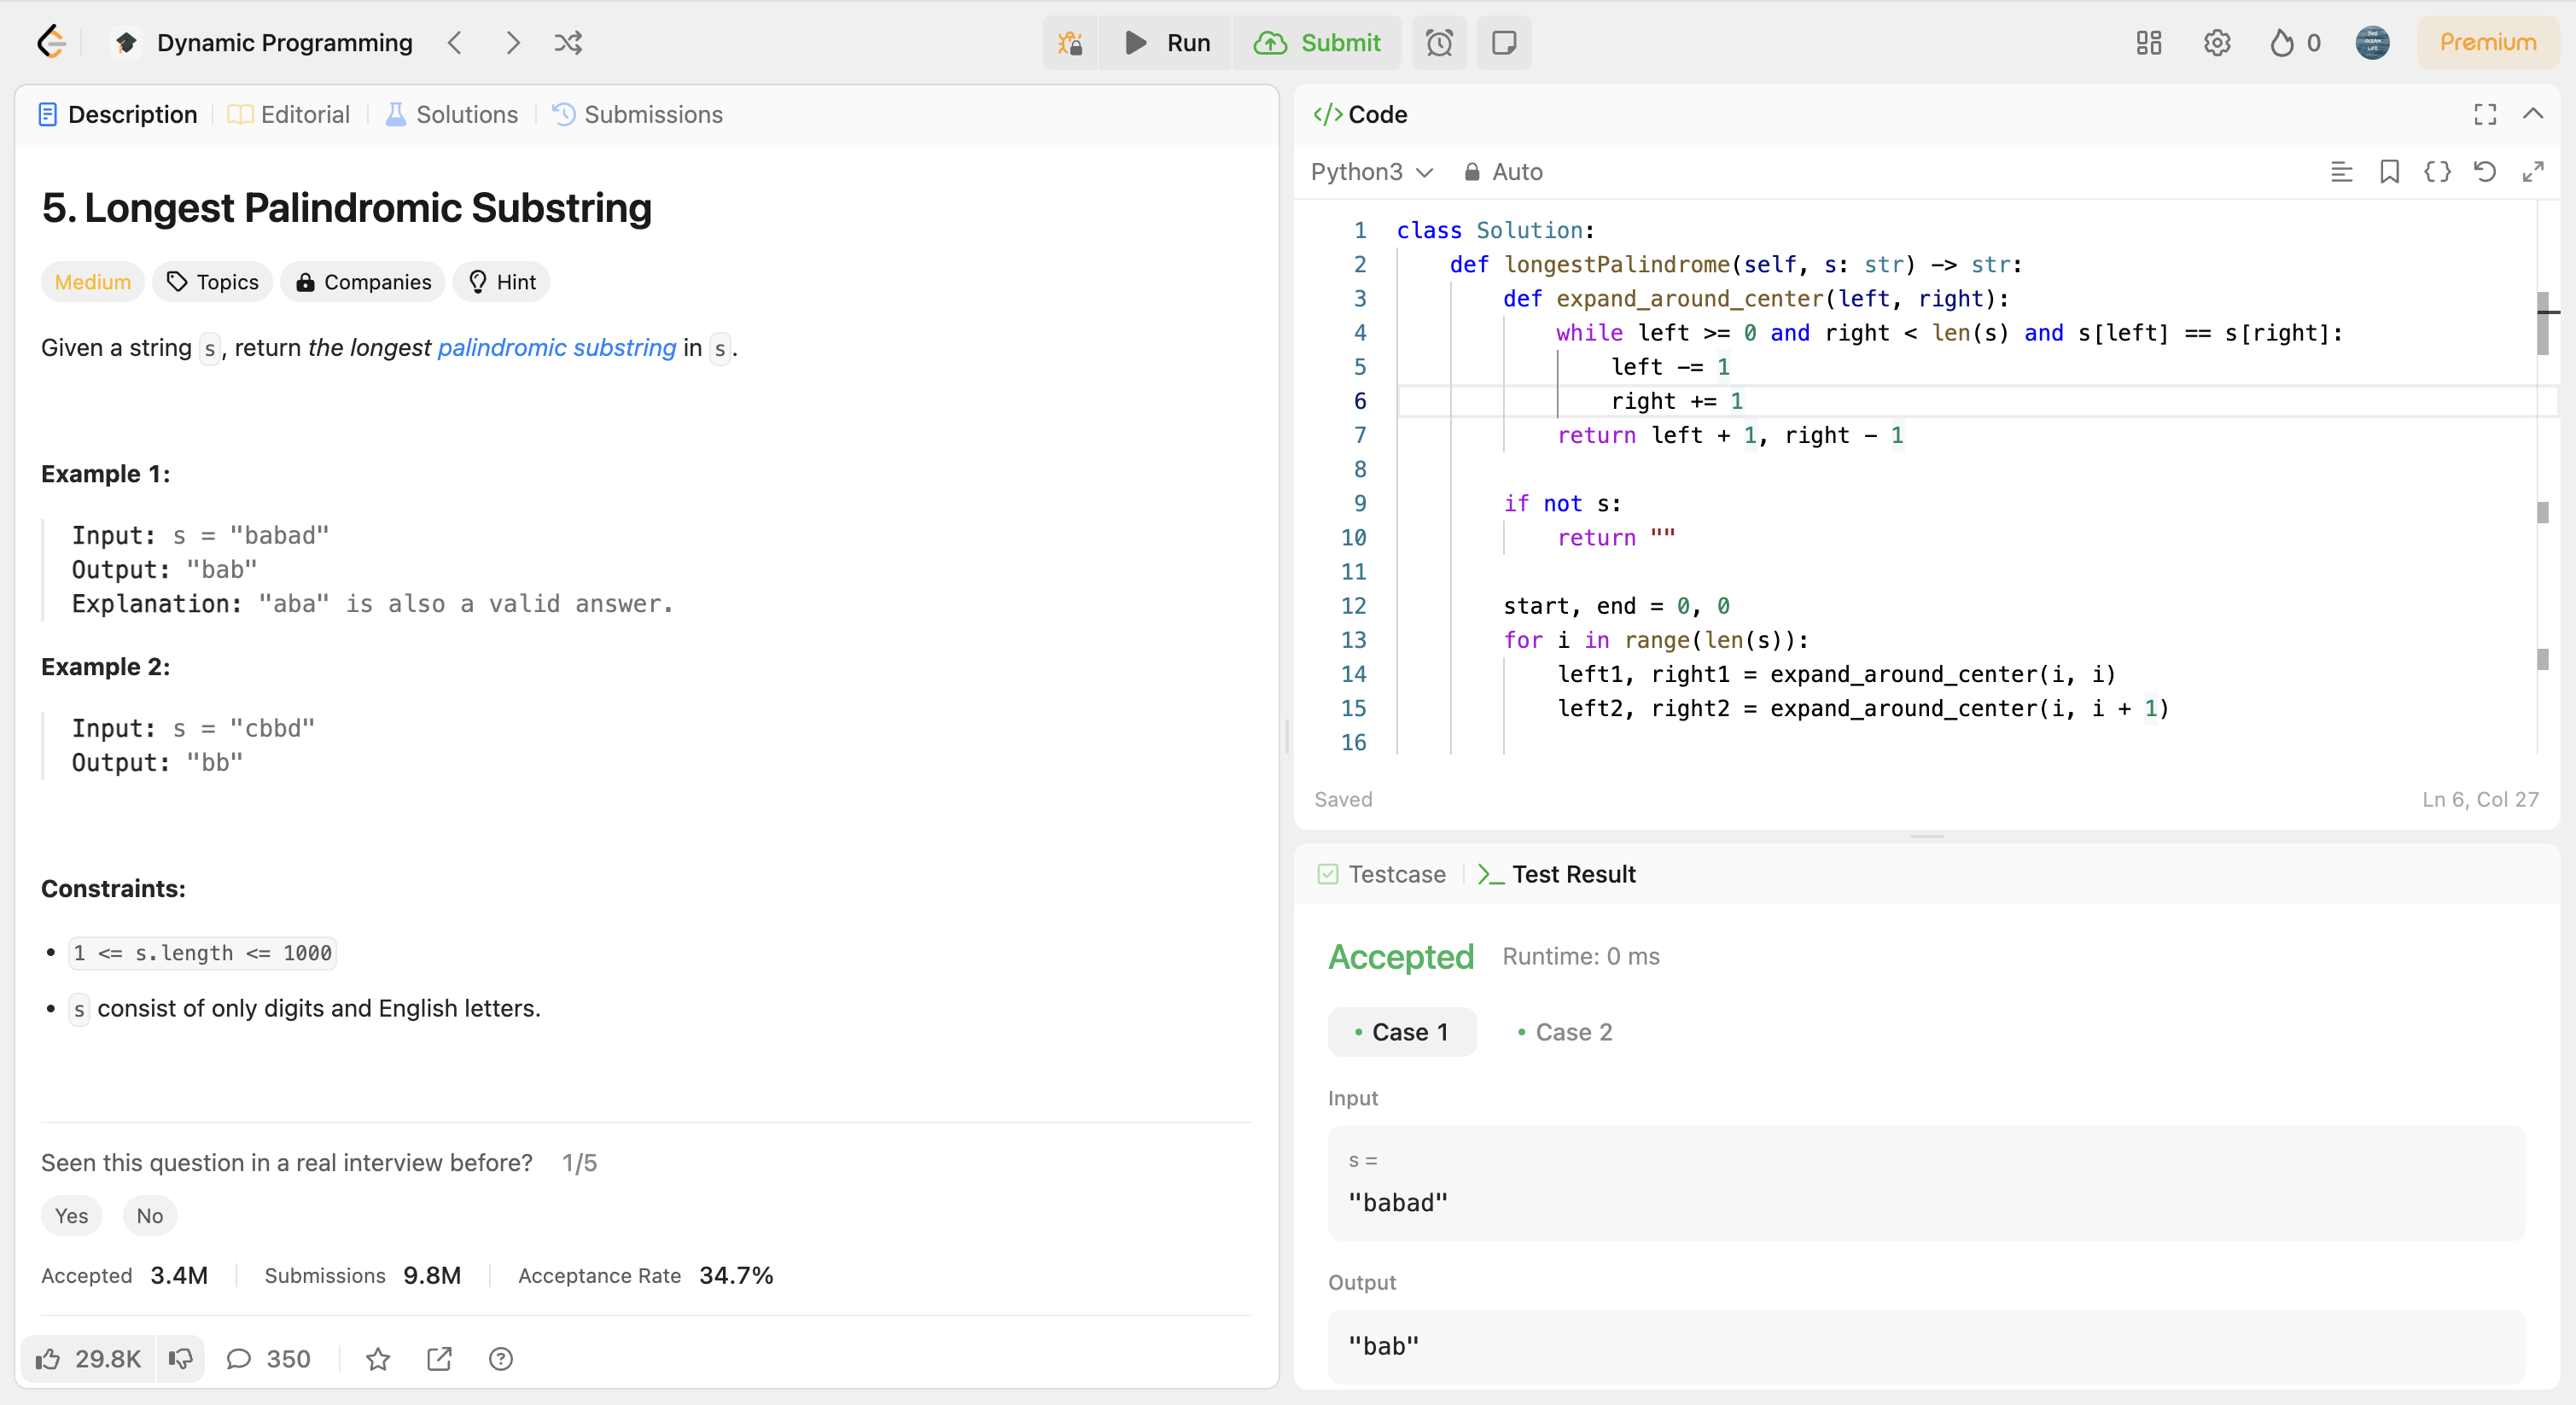
\includegraphics[width=0.95\linewidth]{images/leetcode.jpg}
\caption{\done{An exemplar of GitHub Copilot to demonstrate how to use development tools powered by LLMs, including powerful GPT 4o, o1-preview (Preview), and o1-mini (Preview). 
To illustrate its capabilities, we input the description of the ``5. Longest Palindromic Substring'' problem from LeetCode into Copilot's chat box. 
The code generated by Copilot is then submitted to the online judge platform, where it is successfully accepted.
}}
\label{fig:copilot}
\end{figure*}
\subsection{Applications}\label{sec:application}
Code LLMs have been integrated with development tools and platforms, such as
integrated development environments (IDEs) and version control systems, improving programming efficiency substantially. In this section, we will briefly introduce several widely used applications as coding assistants. The statistics of these applications are provided in Table \ref{tab:products}.
% \subsubsection{OpenAI Code Interpreter}
% \subsubsection{Devin}
% \subsubsection{OpenDevin}

\textbf{GitHub Copilot.}
GitHub Copilot, powered by OpenAI's Codex, is an AI pair programmer that helps you write better code faster. Copilot suggests whole lines or blocks of code as you type, based on the context provided by your existing code and comments. It's trained on a dataset that includes a significant portion of the public code available on GitHub, which enables it to understand a wide range of programming languages and coding styles. Copilot not only improves productivity but also serves as a learning tool by providing programmers with examples of how certain functions can be implemented or how specific problems can be solved.

\textbf{CodeGeeX.}
% CodeGeeX is a versatile programming assistant capable of completing code, generating comments, translating code, and communicating with developers. This intelligent assistant, driven by a powerful code generation LLM, is trained on massive code tokens and demonstrates exceptional performances on the HumanEval, HumanEval-X, and DS1000 benchmarks. CodeGeeX is renowned for its capability to support multilingual code generation tasks, which helps to significantly improve code development efficiency.
CodeGeeX stands out as a multifaceted programming assistant, proficient in code completion, comment generation, code translation, and developer interactions. 
Its underlying code generation LLM has been refined with extensive training on vast amounts of code data, exhibiting superior performance on benchmarks like HumanEval, HumanEval-X, and DS1000. 
Renowned for supporting multilingual code generation, CodeGeeX plays a pivotal role in enhancing the efficiency of code development.

\textbf{CodeWhisperer.}
% Amazon CodeWhisperer is a general-purpose, machine learning-powered code generator that provides you with code recommendations in real time. As you write code, CodeWhisperer automatically generates suggestions based on your existing code and comments. Your personalized recommendations can vary in size and scope, ranging from a single-line comment to fully formed functions.
Amazon's CodeWhisperer is a versatile, machine learning-driven code generator that offers on-the-fly code recommendations. Tailored to your coding patterns and comments, CodeWhisperer provides personalized suggestions that range from succinct comments to complex functions, all aimed at streamlining your coding workflow.

\textbf{Codeium.}
% Codeium accelerates the process of code development with advanced AI. This helpful toolkit leverages different models to provide functions such as code completion, explanation, translation, searching, and user chatting. Codeium provides various capabilities in more than 70 languages, with fast speeds and state-of-the-art quality, helping users to solve code-related problems with ease. 
Codeium is an AI-accelerated coding toolkit that offers a suite of functions, including code completion, explanation, translation, search, and user chatting. Compatible with over 70 programming languages, Codeium delivers fast and cutting-edge solutions to coding challenges, simplifying the development process for its users.

\textbf{CodeArts Snap.}
% Huawei CodeArts Snap can generate complete function-level code based on Chinese and English descriptions, which can replace repetitive and tedious manual coding, efficiently generate test code, and also provide automatic code checking and repair.
Huawei's CodeArts Snap is capable of generating comprehensive function-level code from both Chinese and English descriptions. This tool not only reduces the monotony of manual coding but also efficiently generates test code, in addition to providing automatic code analysis and repair services.

\textbf{Tabnine.}
% Tabnine is the AI coding assistant that helps development teams of every size use AI to accelerate and simplify the software development process without sacrificing privacy, security, or compliance. 
% Tabnine boosts engineering velocity, code quality, and developer happiness by automating the coding workflow through AI tools customized to your team. Tabnine supports more than one million developers across companies in every industry.
Tabnine is an AI coding assistant that empowers development teams to leverage AI for streamlining the software development lifecycle while maintaining strict standards for privacy, security, and compliance. With a focus on enhancing coding efficiency, code quality, and developer satisfaction, Tabnine offers AI-driven automation that is tailored to the needs of your team. Supporting over one million developers worldwide, Tabnine is applicable across various industries.

\textbf{Replit.}
% Replit provides a large range of tools and features necessary for software development. It serves as a free online IDE, a code collaboration platform, a cloud provider, a developer community, and so much more. Besides, Replit allows you to quickly compile and execute code in over 50 programming languages in your browser, without downloading anything to your computer.
Replit is a multifunctional platform that caters to a diverse array of software development needs. As a complimentary online IDE, it facilitates code collaboration, and cloud services, and fosters a thriving developer community. Replit also enables users to compile and execute code in more than 50 programming languages directly within a web browser, eliminating the need for local software installations.


\done{
To illustrate the use of development tools powered by LLMs, we employ GitHub Copilot within Visual Studio Code (VS Code) as our example. Note that 
\begin{itemize}
    \item [\textcircled{1}] For details on using the GitHub Copilot extension in VS Code, please refer to the useful document at \href{https://code.visualstudio.com/docs/copilot/overview}{https://code.visualstudio.com/docs/copilot/overview}. 
    \item [\textcircled{2}] If you would like to get free access to Copilot as a student, teacher, or open-source maintainer, please refer to this tutorial at \href{https://docs.github.com/en/copilot/managing-copilot/managing-copilot-as-an-individual-subscriber/managing-your-copilot-subscription/getting-free-access-to-copilot-as-a-student-teacher-or-maintainer}{https://docs.github.com/en/copilot/managing-copilot/managing-copilot-as-an-individual-subscriber/managing-your-copilot-subscription/getting-free-access-to-copilot-as-a-student-teacher-or-maintainer} and GitHub education application portal at \\ \href{https://education.github.com/discount_requests/application}{https://education.github.com/discount\_requests/application}.
\end{itemize}
As depicted in the upper section of Figure \ref{fig:copilot}, users can interact with Copilot through the chat box in the lower left corner, where they can inquire about various coding-related tasks. 
This feature is now supported by the advanced capabilities of GPT-4o, o1-preview (Preview), and o1-mini (Preview).
From the generated content, Copilot demonstrates the ability to plan solutions to coding problems. It can write code and subsequently explain the generated code to enhance user comprehension. 
Within the right-side workspace, users can engage in inline chat conversations to generate or refactor source code, conduct code explanations, fix coding errors, resolve issues encountered during terminal command executions, produce documentation comments, and generate unit tests.
To illustrate its capabilities, we input the description of the ``5. Longest Palindromic Substring'' problem from LeetCode into Copilot's chat box. 
The code generated by Copilot is then submitted to the online judge platform, where it is successfully accepted, as shown at the lower section of Figure \ref{fig:copilot}.
}
% The GitHub Copilot extension is an AI pair programmer tool that helps you write code faster and smarter. You can use the Copilot extension in Visual Studio Code to generate code, learn from the code it generates, and even configure your editor.
% With GitHub Copilot in VS Code you can:
% Get inline code suggestions while you're writing and iterating on code.
% Start a chat conversation to generate or refactor source code, produce documentation comments, or generate unit tests.
% Get help with fixing errors in your code, or resolve errors while running commands in the terminal.
% Ask questions to help ramp-up on a new code base, or accelerate learning a new programming language or framework.
% Use chat features to discover and configure your VS Code setup.